
% Default to the notebook output style



% Tell the templating engine what output template we want to use.

% Default to the notebook output style


% Inherit from the specified cell style.




    
\documentclass{article}

    
    
    \usepackage{graphicx} % Used to insert images
    \usepackage{adjustbox} % Used to constrain images to a maximum size 
    \usepackage{color} % Allow colors to be defined
    \usepackage{enumerate} % Needed for markdown enumerations to work
    \usepackage{geometry} % Used to adjust the document margins
    \usepackage{amsmath} % Equations
    \usepackage{amssymb} % Equations
    \usepackage{eurosym} % defines \euro
    \usepackage[mathletters]{ucs} % Extended unicode (utf-8) support
    \usepackage[utf8x]{inputenc} % Allow utf-8 characters in the tex document
    \usepackage{fancyvrb} % verbatim replacement that allows latex
    \usepackage{grffile} % extends the file name processing of package graphics 
                         % to support a larger range 
    % The hyperref package gives us a pdf with properly built
    % internal navigation ('pdf bookmarks' for the table of contents,
    % internal cross-reference links, web links for URLs, etc.)
    \usepackage{hyperref}
    \usepackage{longtable} % longtable support required by pandoc >1.10
    \usepackage{booktabs}  % table support for pandoc > 1.12.2
    

    
    
    \definecolor{orange}{cmyk}{0,0.4,0.8,0.2}
    \definecolor{darkorange}{rgb}{.71,0.21,0.01}
    \definecolor{darkgreen}{rgb}{.12,.54,.11}
    \definecolor{myteal}{rgb}{.26, .44, .56}
    \definecolor{gray}{gray}{0.45}
    \definecolor{lightgray}{gray}{.95}
    \definecolor{mediumgray}{gray}{.8}
    \definecolor{inputbackground}{rgb}{.95, .95, .85}
    \definecolor{outputbackground}{rgb}{.95, .95, .95}
    \definecolor{traceback}{rgb}{1, .95, .95}
    % ansi colors
    \definecolor{red}{rgb}{.6,0,0}
    \definecolor{green}{rgb}{0,.65,0}
    \definecolor{brown}{rgb}{0.6,0.6,0}
    \definecolor{blue}{rgb}{0,.145,.698}
    \definecolor{purple}{rgb}{.698,.145,.698}
    \definecolor{cyan}{rgb}{0,.698,.698}
    \definecolor{lightgray}{gray}{0.5}
    
    % bright ansi colors
    \definecolor{darkgray}{gray}{0.25}
    \definecolor{lightred}{rgb}{1.0,0.39,0.28}
    \definecolor{lightgreen}{rgb}{0.48,0.99,0.0}
    \definecolor{lightblue}{rgb}{0.53,0.81,0.92}
    \definecolor{lightpurple}{rgb}{0.87,0.63,0.87}
    \definecolor{lightcyan}{rgb}{0.5,1.0,0.83}
    
    % commands and environments needed by pandoc snippets
    % extracted from the output of `pandoc -s`
    \providecommand{\tightlist}{%
      \setlength{\itemsep}{0pt}\setlength{\parskip}{0pt}}
    \DefineVerbatimEnvironment{Highlighting}{Verbatim}{commandchars=\\\{\}}
    % Add ',fontsize=\small' for more characters per line
    \newenvironment{Shaded}{}{}
    \newcommand{\KeywordTok}[1]{\textcolor[rgb]{0.00,0.44,0.13}{\textbf{{#1}}}}
    \newcommand{\DataTypeTok}[1]{\textcolor[rgb]{0.56,0.13,0.00}{{#1}}}
    \newcommand{\DecValTok}[1]{\textcolor[rgb]{0.25,0.63,0.44}{{#1}}}
    \newcommand{\BaseNTok}[1]{\textcolor[rgb]{0.25,0.63,0.44}{{#1}}}
    \newcommand{\FloatTok}[1]{\textcolor[rgb]{0.25,0.63,0.44}{{#1}}}
    \newcommand{\CharTok}[1]{\textcolor[rgb]{0.25,0.44,0.63}{{#1}}}
    \newcommand{\StringTok}[1]{\textcolor[rgb]{0.25,0.44,0.63}{{#1}}}
    \newcommand{\CommentTok}[1]{\textcolor[rgb]{0.38,0.63,0.69}{\textit{{#1}}}}
    \newcommand{\OtherTok}[1]{\textcolor[rgb]{0.00,0.44,0.13}{{#1}}}
    \newcommand{\AlertTok}[1]{\textcolor[rgb]{1.00,0.00,0.00}{\textbf{{#1}}}}
    \newcommand{\FunctionTok}[1]{\textcolor[rgb]{0.02,0.16,0.49}{{#1}}}
    \newcommand{\RegionMarkerTok}[1]{{#1}}
    \newcommand{\ErrorTok}[1]{\textcolor[rgb]{1.00,0.00,0.00}{\textbf{{#1}}}}
    \newcommand{\NormalTok}[1]{{#1}}
    
    % Define a nice break command that doesn't care if a line doesn't already
    % exist.
    \def\br{\hspace*{\fill} \\* }
    % Math Jax compatability definitions
    \def\gt{>}
    \def\lt{<}
    % Document parameters
    \title{england}
    
    
    

    % Pygments definitions
    
\makeatletter
\def\PY@reset{\let\PY@it=\relax \let\PY@bf=\relax%
    \let\PY@ul=\relax \let\PY@tc=\relax%
    \let\PY@bc=\relax \let\PY@ff=\relax}
\def\PY@tok#1{\csname PY@tok@#1\endcsname}
\def\PY@toks#1+{\ifx\relax#1\empty\else%
    \PY@tok{#1}\expandafter\PY@toks\fi}
\def\PY@do#1{\PY@bc{\PY@tc{\PY@ul{%
    \PY@it{\PY@bf{\PY@ff{#1}}}}}}}
\def\PY#1#2{\PY@reset\PY@toks#1+\relax+\PY@do{#2}}

\expandafter\def\csname PY@tok@gd\endcsname{\def\PY@tc##1{\textcolor[rgb]{0.63,0.00,0.00}{##1}}}
\expandafter\def\csname PY@tok@gu\endcsname{\let\PY@bf=\textbf\def\PY@tc##1{\textcolor[rgb]{0.50,0.00,0.50}{##1}}}
\expandafter\def\csname PY@tok@gt\endcsname{\def\PY@tc##1{\textcolor[rgb]{0.00,0.27,0.87}{##1}}}
\expandafter\def\csname PY@tok@gs\endcsname{\let\PY@bf=\textbf}
\expandafter\def\csname PY@tok@gr\endcsname{\def\PY@tc##1{\textcolor[rgb]{1.00,0.00,0.00}{##1}}}
\expandafter\def\csname PY@tok@cm\endcsname{\let\PY@it=\textit\def\PY@tc##1{\textcolor[rgb]{0.25,0.50,0.50}{##1}}}
\expandafter\def\csname PY@tok@vg\endcsname{\def\PY@tc##1{\textcolor[rgb]{0.10,0.09,0.49}{##1}}}
\expandafter\def\csname PY@tok@m\endcsname{\def\PY@tc##1{\textcolor[rgb]{0.40,0.40,0.40}{##1}}}
\expandafter\def\csname PY@tok@mh\endcsname{\def\PY@tc##1{\textcolor[rgb]{0.40,0.40,0.40}{##1}}}
\expandafter\def\csname PY@tok@go\endcsname{\def\PY@tc##1{\textcolor[rgb]{0.53,0.53,0.53}{##1}}}
\expandafter\def\csname PY@tok@ge\endcsname{\let\PY@it=\textit}
\expandafter\def\csname PY@tok@vc\endcsname{\def\PY@tc##1{\textcolor[rgb]{0.10,0.09,0.49}{##1}}}
\expandafter\def\csname PY@tok@il\endcsname{\def\PY@tc##1{\textcolor[rgb]{0.40,0.40,0.40}{##1}}}
\expandafter\def\csname PY@tok@cs\endcsname{\let\PY@it=\textit\def\PY@tc##1{\textcolor[rgb]{0.25,0.50,0.50}{##1}}}
\expandafter\def\csname PY@tok@cp\endcsname{\def\PY@tc##1{\textcolor[rgb]{0.74,0.48,0.00}{##1}}}
\expandafter\def\csname PY@tok@gi\endcsname{\def\PY@tc##1{\textcolor[rgb]{0.00,0.63,0.00}{##1}}}
\expandafter\def\csname PY@tok@gh\endcsname{\let\PY@bf=\textbf\def\PY@tc##1{\textcolor[rgb]{0.00,0.00,0.50}{##1}}}
\expandafter\def\csname PY@tok@ni\endcsname{\let\PY@bf=\textbf\def\PY@tc##1{\textcolor[rgb]{0.60,0.60,0.60}{##1}}}
\expandafter\def\csname PY@tok@nl\endcsname{\def\PY@tc##1{\textcolor[rgb]{0.63,0.63,0.00}{##1}}}
\expandafter\def\csname PY@tok@nn\endcsname{\let\PY@bf=\textbf\def\PY@tc##1{\textcolor[rgb]{0.00,0.00,1.00}{##1}}}
\expandafter\def\csname PY@tok@no\endcsname{\def\PY@tc##1{\textcolor[rgb]{0.53,0.00,0.00}{##1}}}
\expandafter\def\csname PY@tok@na\endcsname{\def\PY@tc##1{\textcolor[rgb]{0.49,0.56,0.16}{##1}}}
\expandafter\def\csname PY@tok@nb\endcsname{\def\PY@tc##1{\textcolor[rgb]{0.00,0.50,0.00}{##1}}}
\expandafter\def\csname PY@tok@nc\endcsname{\let\PY@bf=\textbf\def\PY@tc##1{\textcolor[rgb]{0.00,0.00,1.00}{##1}}}
\expandafter\def\csname PY@tok@nd\endcsname{\def\PY@tc##1{\textcolor[rgb]{0.67,0.13,1.00}{##1}}}
\expandafter\def\csname PY@tok@ne\endcsname{\let\PY@bf=\textbf\def\PY@tc##1{\textcolor[rgb]{0.82,0.25,0.23}{##1}}}
\expandafter\def\csname PY@tok@nf\endcsname{\def\PY@tc##1{\textcolor[rgb]{0.00,0.00,1.00}{##1}}}
\expandafter\def\csname PY@tok@si\endcsname{\let\PY@bf=\textbf\def\PY@tc##1{\textcolor[rgb]{0.73,0.40,0.53}{##1}}}
\expandafter\def\csname PY@tok@s2\endcsname{\def\PY@tc##1{\textcolor[rgb]{0.73,0.13,0.13}{##1}}}
\expandafter\def\csname PY@tok@vi\endcsname{\def\PY@tc##1{\textcolor[rgb]{0.10,0.09,0.49}{##1}}}
\expandafter\def\csname PY@tok@nt\endcsname{\let\PY@bf=\textbf\def\PY@tc##1{\textcolor[rgb]{0.00,0.50,0.00}{##1}}}
\expandafter\def\csname PY@tok@nv\endcsname{\def\PY@tc##1{\textcolor[rgb]{0.10,0.09,0.49}{##1}}}
\expandafter\def\csname PY@tok@s1\endcsname{\def\PY@tc##1{\textcolor[rgb]{0.73,0.13,0.13}{##1}}}
\expandafter\def\csname PY@tok@kd\endcsname{\let\PY@bf=\textbf\def\PY@tc##1{\textcolor[rgb]{0.00,0.50,0.00}{##1}}}
\expandafter\def\csname PY@tok@sh\endcsname{\def\PY@tc##1{\textcolor[rgb]{0.73,0.13,0.13}{##1}}}
\expandafter\def\csname PY@tok@sc\endcsname{\def\PY@tc##1{\textcolor[rgb]{0.73,0.13,0.13}{##1}}}
\expandafter\def\csname PY@tok@sx\endcsname{\def\PY@tc##1{\textcolor[rgb]{0.00,0.50,0.00}{##1}}}
\expandafter\def\csname PY@tok@bp\endcsname{\def\PY@tc##1{\textcolor[rgb]{0.00,0.50,0.00}{##1}}}
\expandafter\def\csname PY@tok@c1\endcsname{\let\PY@it=\textit\def\PY@tc##1{\textcolor[rgb]{0.25,0.50,0.50}{##1}}}
\expandafter\def\csname PY@tok@kc\endcsname{\let\PY@bf=\textbf\def\PY@tc##1{\textcolor[rgb]{0.00,0.50,0.00}{##1}}}
\expandafter\def\csname PY@tok@c\endcsname{\let\PY@it=\textit\def\PY@tc##1{\textcolor[rgb]{0.25,0.50,0.50}{##1}}}
\expandafter\def\csname PY@tok@mf\endcsname{\def\PY@tc##1{\textcolor[rgb]{0.40,0.40,0.40}{##1}}}
\expandafter\def\csname PY@tok@err\endcsname{\def\PY@bc##1{\setlength{\fboxsep}{0pt}\fcolorbox[rgb]{1.00,0.00,0.00}{1,1,1}{\strut ##1}}}
\expandafter\def\csname PY@tok@mb\endcsname{\def\PY@tc##1{\textcolor[rgb]{0.40,0.40,0.40}{##1}}}
\expandafter\def\csname PY@tok@ss\endcsname{\def\PY@tc##1{\textcolor[rgb]{0.10,0.09,0.49}{##1}}}
\expandafter\def\csname PY@tok@sr\endcsname{\def\PY@tc##1{\textcolor[rgb]{0.73,0.40,0.53}{##1}}}
\expandafter\def\csname PY@tok@mo\endcsname{\def\PY@tc##1{\textcolor[rgb]{0.40,0.40,0.40}{##1}}}
\expandafter\def\csname PY@tok@kn\endcsname{\let\PY@bf=\textbf\def\PY@tc##1{\textcolor[rgb]{0.00,0.50,0.00}{##1}}}
\expandafter\def\csname PY@tok@mi\endcsname{\def\PY@tc##1{\textcolor[rgb]{0.40,0.40,0.40}{##1}}}
\expandafter\def\csname PY@tok@gp\endcsname{\let\PY@bf=\textbf\def\PY@tc##1{\textcolor[rgb]{0.00,0.00,0.50}{##1}}}
\expandafter\def\csname PY@tok@o\endcsname{\def\PY@tc##1{\textcolor[rgb]{0.40,0.40,0.40}{##1}}}
\expandafter\def\csname PY@tok@kr\endcsname{\let\PY@bf=\textbf\def\PY@tc##1{\textcolor[rgb]{0.00,0.50,0.00}{##1}}}
\expandafter\def\csname PY@tok@s\endcsname{\def\PY@tc##1{\textcolor[rgb]{0.73,0.13,0.13}{##1}}}
\expandafter\def\csname PY@tok@kp\endcsname{\def\PY@tc##1{\textcolor[rgb]{0.00,0.50,0.00}{##1}}}
\expandafter\def\csname PY@tok@w\endcsname{\def\PY@tc##1{\textcolor[rgb]{0.73,0.73,0.73}{##1}}}
\expandafter\def\csname PY@tok@kt\endcsname{\def\PY@tc##1{\textcolor[rgb]{0.69,0.00,0.25}{##1}}}
\expandafter\def\csname PY@tok@ow\endcsname{\let\PY@bf=\textbf\def\PY@tc##1{\textcolor[rgb]{0.67,0.13,1.00}{##1}}}
\expandafter\def\csname PY@tok@sb\endcsname{\def\PY@tc##1{\textcolor[rgb]{0.73,0.13,0.13}{##1}}}
\expandafter\def\csname PY@tok@k\endcsname{\let\PY@bf=\textbf\def\PY@tc##1{\textcolor[rgb]{0.00,0.50,0.00}{##1}}}
\expandafter\def\csname PY@tok@se\endcsname{\let\PY@bf=\textbf\def\PY@tc##1{\textcolor[rgb]{0.73,0.40,0.13}{##1}}}
\expandafter\def\csname PY@tok@sd\endcsname{\let\PY@it=\textit\def\PY@tc##1{\textcolor[rgb]{0.73,0.13,0.13}{##1}}}

\def\PYZbs{\char`\\}
\def\PYZus{\char`\_}
\def\PYZob{\char`\{}
\def\PYZcb{\char`\}}
\def\PYZca{\char`\^}
\def\PYZam{\char`\&}
\def\PYZlt{\char`\<}
\def\PYZgt{\char`\>}
\def\PYZsh{\char`\#}
\def\PYZpc{\char`\%}
\def\PYZdl{\char`\$}
\def\PYZhy{\char`\-}
\def\PYZsq{\char`\'}
\def\PYZdq{\char`\"}
\def\PYZti{\char`\~}
% for compatibility with earlier versions
\def\PYZat{@}
\def\PYZlb{[}
\def\PYZrb{]}
\makeatother


    % Exact colors from NB
    \definecolor{incolor}{rgb}{0.0, 0.0, 0.5}
    \definecolor{outcolor}{rgb}{0.545, 0.0, 0.0}



    
    % Prevent overflowing lines due to hard-to-break entities
    \sloppy 
    % Setup hyperref package
    \hypersetup{
      breaklinks=true,  % so long urls are correctly broken across lines
      colorlinks=true,
      urlcolor=blue,
      linkcolor=darkorange,
      citecolor=darkgreen,
      }
    % Slightly bigger margins than the latex defaults
    
    \geometry{verbose,tmargin=1in,bmargin=1in,lmargin=1in,rmargin=1in}
    
    

    \begin{document}
    
    
    \author{Joanna Lewis and Peter White}\title{Estimating local chlamydia incidence and prevalence using surveillance data: eAppendix 2}

\date{\today}
\maketitle

\tableofcontents


    
    

    
    \section{Example: Chlamydia in England,
2012}\label{example-chlamydia-in-england-2012}

This example illustrates a method for using chlamydia surveillance data
to estimate prevalence. Surveillance data on chlamydia testing and
diagnosis rates in England in 2012 were downloaded from:
http://www.chlamydiascreening.nhs.uk/ps/data.asp (downloaded 9 February
2016).

\begin{longtable}[c]{@{}lllllll@{}}
\toprule
& Men & & & Women & &\tabularnewline
\midrule
\endhead
& 15-19 years & 20-24 years & Total & 15-19 years & 20-24 years &
Total\tabularnewline
Population & 1685620 & 1833395 & 3519015 & 1600686 & 1788156 &
3388842\tabularnewline
Tests & 232668 & 334240 & 566908 & 520358 & 685538 &
1205896\tabularnewline
Diagnoses & 15213 & 33174 & 48387 & 42874 & 45227 & 88101\tabularnewline
\bottomrule
\end{longtable}

Data on sexual behaviour from the third National Study of Sexual
Attitudes and Lifestyles (Natsal-3) are available from the UK data
service: https://www.ukdataservice.ac.uk/ (downloaded 23 September
2015). These were used to infer 95\% confidence intervals for the
proportions of men and women, aged 16-19 and 20-24, who were sexually
active (see the accompanying R script; note that no 15-year-olds were
recruited to Natsal-3). These 95\% confidence intervals were in turn
used to derive beta-distribution priors for the proportion sexually
active within each sex and age group.

\subsection{Sampling for testing and diagnosis
rates}\label{sampling-for-testing-and-diagnosis-rates}

    \begin{footnotesize}
        \begin{Verbatim}[commandchars=\\\{\}]
{\color{incolor}In [{\color{incolor}1}]:} \PY{k+kn}{import} \PY{n+nn}{numpy} \PY{k+kn}{as} \PY{n+nn}{np}
        \PY{k+kn}{from} \PY{n+nn}{numpy} \PY{k+kn}{import} \PY{o}{*}
        \PY{k+kn}{from} \PY{n+nn}{scipy.stats} \PY{k+kn}{import} \PY{n}{beta}
        \PY{k+kn}{from} \PY{n+nn}{scipy.optimize} \PY{k+kn}{import} \PY{n}{fsolve}
        
        
        \PY{c}{\PYZsh{}\PYZsh{}\PYZsh{}\PYZsh{}\PYZsh{}\PYZsh{}\PYZsh{}\PYZsh{}\PYZsh{}\PYZsh{}\PYZsh{}\PYZsh{}\PYZsh{}\PYZsh{}\PYZsh{}\PYZsh{}\PYZsh{}\PYZsh{}\PYZsh{}\PYZsh{}\PYZsh{}\PYZsh{}}
        \PY{c}{\PYZsh{} parameters of beta distributions representing the proportion of the population sexually }
        \PY{c}{\PYZsh{} active, by sex and age group}
        \PY{c}{\PYZsh{}\PYZsh{}\PYZsh{}\PYZsh{}\PYZsh{}\PYZsh{}\PYZsh{}\PYZsh{}\PYZsh{}\PYZsh{}\PYZsh{}\PYZsh{}\PYZsh{}\PYZsh{}\PYZsh{}\PYZsh{}\PYZsh{}\PYZsh{}\PYZsh{}\PYZsh{}\PYZsh{}\PYZsh{}}
        
        \PY{c}{\PYZsh{} men, 16\PYZhy{}19}
        \PY{p}{[}\PY{n}{alpha\PYZus{}m\PYZus{}16\PYZus{}19}\PY{p}{,} \PY{n}{beta\PYZus{}m\PYZus{}16\PYZus{}19}\PY{p}{]} \PY{o}{=} \PY{n}{fsolve}\PY{p}{(}
            \PY{k}{lambda} \PY{n}{x}\PY{p}{:} \PY{n}{array}\PY{p}{(}\PY{n}{beta}\PY{o}{.}\PY{n}{interval}\PY{p}{(}\PY{l+m+mf}{0.95}\PY{p}{,} \PY{n}{x}\PY{p}{[}\PY{l+m+mi}{0}\PY{p}{]}\PY{p}{,} \PY{n}{x}\PY{p}{[}\PY{l+m+mi}{1}\PY{p}{]}\PY{p}{,} \PY{n}{loc}\PY{o}{=}\PY{l+m+mi}{0}\PY{p}{,} \PY{n}{scale}\PY{o}{=}\PY{l+m+mi}{1}\PY{p}{)}\PY{p}{)}
            \PY{o}{\PYZhy{}} \PY{p}{(}\PY{l+m+mf}{0.6747424}\PY{p}{,} \PY{l+m+mf}{0.741327698}\PY{p}{)}\PY{p}{,}
            \PY{p}{[}\PY{l+m+mi}{1}\PY{p}{,}\PY{l+m+mi}{1}\PY{p}{]}
            \PY{p}{)}
        \PY{c}{\PYZsh{} men, 20\PYZhy{}24}
        \PY{p}{[}\PY{n}{alpha\PYZus{}m\PYZus{}20\PYZus{}24}\PY{p}{,} \PY{n}{beta\PYZus{}m\PYZus{}20\PYZus{}24}\PY{p}{]} \PY{o}{=} \PY{n}{fsolve}\PY{p}{(}
            \PY{k}{lambda} \PY{n}{x}\PY{p}{:} \PY{n}{array}\PY{p}{(}\PY{n}{beta}\PY{o}{.}\PY{n}{interval}\PY{p}{(}\PY{l+m+mf}{0.95}\PY{p}{,} \PY{n}{x}\PY{p}{[}\PY{l+m+mi}{0}\PY{p}{]}\PY{p}{,} \PY{n}{x}\PY{p}{[}\PY{l+m+mi}{1}\PY{p}{]}\PY{p}{,} \PY{n}{loc}\PY{o}{=}\PY{l+m+mi}{0}\PY{p}{,} \PY{n}{scale}\PY{o}{=}\PY{l+m+mi}{1}\PY{p}{)}\PY{p}{)}
            \PY{o}{\PYZhy{}} \PY{p}{(}\PY{l+m+mf}{0.8844970}\PY{p}{,} \PY{l+m+mf}{0.933759842}\PY{p}{)}\PY{p}{,}
            \PY{p}{[}\PY{l+m+mi}{1}\PY{p}{,}\PY{l+m+mi}{1}\PY{p}{]}
            \PY{p}{)}
        \PY{c}{\PYZsh{} men, 16\PYZhy{}24}
        \PY{p}{[}\PY{n}{alpha\PYZus{}m\PYZus{}16\PYZus{}24}\PY{p}{,} \PY{n}{beta\PYZus{}m\PYZus{}16\PYZus{}24}\PY{p}{]} \PY{o}{=} \PY{n}{fsolve}\PY{p}{(}
            \PY{k}{lambda} \PY{n}{x}\PY{p}{:} \PY{n}{array}\PY{p}{(}\PY{n}{beta}\PY{o}{.}\PY{n}{interval}\PY{p}{(}\PY{l+m+mf}{0.95}\PY{p}{,} \PY{n}{x}\PY{p}{[}\PY{l+m+mi}{0}\PY{p}{]}\PY{p}{,} \PY{n}{x}\PY{p}{[}\PY{l+m+mi}{1}\PY{p}{]}\PY{p}{,} \PY{n}{loc}\PY{o}{=}\PY{l+m+mi}{0}\PY{p}{,} \PY{n}{scale}\PY{o}{=}\PY{l+m+mi}{1}\PY{p}{)}\PY{p}{)}
            \PY{o}{\PYZhy{}} \PY{p}{(}\PY{l+m+mf}{0.8023836019}\PY{p}{,} \PY{l+m+mf}{0.843403825}\PY{p}{)}\PY{p}{,}
            \PY{p}{[}\PY{l+m+mi}{1}\PY{p}{,}\PY{l+m+mi}{1}\PY{p}{]}
            \PY{p}{)}
        \PY{c}{\PYZsh{} women, 16\PYZhy{}19}
        \PY{p}{[}\PY{n}{alpha\PYZus{}f\PYZus{}16\PYZus{}19}\PY{p}{,} \PY{n}{beta\PYZus{}f\PYZus{}16\PYZus{}19}\PY{p}{]} \PY{o}{=} \PY{n}{fsolve}\PY{p}{(}
            \PY{k}{lambda} \PY{n}{x}\PY{p}{:} \PY{n}{array}\PY{p}{(}\PY{n}{beta}\PY{o}{.}\PY{n}{interval}\PY{p}{(}\PY{l+m+mf}{0.95}\PY{p}{,} \PY{n}{x}\PY{p}{[}\PY{l+m+mi}{0}\PY{p}{]}\PY{p}{,} \PY{n}{x}\PY{p}{[}\PY{l+m+mi}{1}\PY{p}{]}\PY{p}{,} \PY{n}{loc}\PY{o}{=}\PY{l+m+mi}{0}\PY{p}{,} \PY{n}{scale}\PY{o}{=}\PY{l+m+mi}{1}\PY{p}{)}\PY{p}{)}
            \PY{o}{\PYZhy{}} \PY{p}{(}\PY{l+m+mf}{0.6583593}\PY{p}{,} \PY{l+m+mf}{0.723554878}\PY{p}{)}\PY{p}{,}
            \PY{p}{[}\PY{l+m+mi}{1}\PY{p}{,}\PY{l+m+mi}{1}\PY{p}{]}
            \PY{p}{)}
        \PY{c}{\PYZsh{} women, 20\PYZhy{}24}
        \PY{p}{[}\PY{n}{alpha\PYZus{}f\PYZus{}20\PYZus{}24}\PY{p}{,} \PY{n}{beta\PYZus{}f\PYZus{}20\PYZus{}24}\PY{p}{]} \PY{o}{=} \PY{n}{fsolve}\PY{p}{(}
            \PY{k}{lambda} \PY{n}{x}\PY{p}{:} \PY{n}{array}\PY{p}{(}\PY{n}{beta}\PY{o}{.}\PY{n}{interval}\PY{p}{(}\PY{l+m+mf}{0.95}\PY{p}{,} \PY{n}{x}\PY{p}{[}\PY{l+m+mi}{0}\PY{p}{]}\PY{p}{,} \PY{n}{x}\PY{p}{[}\PY{l+m+mi}{1}\PY{p}{]}\PY{p}{,} \PY{n}{loc}\PY{o}{=}\PY{l+m+mi}{0}\PY{p}{,} \PY{n}{scale}\PY{o}{=}\PY{l+m+mi}{1}\PY{p}{)}\PY{p}{)}
            \PY{o}{\PYZhy{}} \PY{p}{(}\PY{l+m+mf}{0.8904135}\PY{p}{,} \PY{l+m+mf}{0.934417684}\PY{p}{)}\PY{p}{,}
            \PY{p}{[}\PY{l+m+mi}{1}\PY{p}{,}\PY{l+m+mi}{1}\PY{p}{]}
            \PY{p}{)}
        \PY{c}{\PYZsh{} women, 16\PYZhy{}24}
        \PY{p}{[}\PY{n}{alpha\PYZus{}f\PYZus{}16\PYZus{}24}\PY{p}{,} \PY{n}{beta\PYZus{}f\PYZus{}16\PYZus{}24}\PY{p}{]} \PY{o}{=} \PY{n}{fsolve}\PY{p}{(}
            \PY{k}{lambda} \PY{n}{x}\PY{p}{:} \PY{n}{array}\PY{p}{(}\PY{n}{beta}\PY{o}{.}\PY{n}{interval}\PY{p}{(}\PY{l+m+mf}{0.95}\PY{p}{,} \PY{n}{x}\PY{p}{[}\PY{l+m+mi}{0}\PY{p}{]}\PY{p}{,} \PY{n}{x}\PY{p}{[}\PY{l+m+mi}{1}\PY{p}{]}\PY{p}{,} \PY{n}{loc}\PY{o}{=}\PY{l+m+mi}{0}\PY{p}{,} \PY{n}{scale}\PY{o}{=}\PY{l+m+mi}{1}\PY{p}{)}\PY{p}{)}
            \PY{o}{\PYZhy{}} \PY{p}{(}\PY{l+m+mf}{0.7998634469}\PY{p}{,} \PY{l+m+mf}{0.837979601}\PY{p}{)}\PY{p}{,}
            \PY{p}{[}\PY{l+m+mi}{1}\PY{p}{,}\PY{l+m+mi}{1}\PY{p}{]}
            \PY{p}{)}
\end{Verbatim}
    \end{footnotesize}

    Next, sample from distributions for the probability of being sexually
active, the size of the sexually active population and the testing and
diagnosis rates per person per year.

    \begin{footnotesize}
        \begin{Verbatim}[commandchars=\\\{\}]
{\color{incolor}In [{\color{incolor}2}]:} \PY{k+kn}{from} \PY{n+nn}{scipy.stats} \PY{k+kn}{import} \PY{n}{gamma}
        \PY{k+kn}{from} \PY{n+nn}{numpy.random} \PY{k+kn}{import} \PY{n}{normal}
        \PY{n}{rs} \PY{o}{=} \PY{n}{random}\PY{o}{.}\PY{n}{RandomState}\PY{p}{(}\PY{l+m+mi}{12345}\PY{p}{)}
        
        \PY{n}{n\PYZus{}sample} \PY{o}{=} \PY{l+m+mi}{10000}
        
        \PY{c}{\PYZsh{} sexually\PYZhy{}active populations:}
        \PY{n}{p\PYZus{}active\PYZus{}m\PYZus{}16\PYZus{}19} \PY{o}{=} \PY{n}{rs}\PY{o}{.}\PY{n}{beta}\PY{p}{(}\PY{n}{alpha\PYZus{}m\PYZus{}16\PYZus{}19}\PY{p}{,} \PY{n}{beta\PYZus{}m\PYZus{}16\PYZus{}19}\PY{p}{,} \PY{n}{size}\PY{o}{=}\PY{n}{n\PYZus{}sample}\PY{p}{)} \PY{c}{\PYZsh{} 16\PYZhy{}19 yo only}
        \PY{n}{pop\PYZus{}active\PYZus{}m\PYZus{}15\PYZus{}19} \PY{o}{=} \PY{n}{rs}\PY{o}{.}\PY{n}{binomial}\PY{p}{(}\PY{l+m+mi}{1685620}\PY{p}{,} \PY{n}{p\PYZus{}active\PYZus{}m\PYZus{}16\PYZus{}19}\PY{p}{,} \PY{n}{size}\PY{o}{=}\PY{n}{n\PYZus{}sample}\PY{p}{)}
        
        \PY{n}{p\PYZus{}active\PYZus{}m\PYZus{}20\PYZus{}24} \PY{o}{=} \PY{n}{rs}\PY{o}{.}\PY{n}{beta}\PY{p}{(}\PY{n}{alpha\PYZus{}m\PYZus{}20\PYZus{}24}\PY{p}{,} \PY{n}{beta\PYZus{}m\PYZus{}20\PYZus{}24}\PY{p}{,} \PY{n}{size}\PY{o}{=}\PY{n}{n\PYZus{}sample}\PY{p}{)} \PY{c}{\PYZsh{} 20\PYZhy{}24 yo only}
        \PY{n}{pop\PYZus{}active\PYZus{}m\PYZus{}20\PYZus{}24} \PY{o}{=} \PY{n}{rs}\PY{o}{.}\PY{n}{binomial}\PY{p}{(}\PY{l+m+mi}{1833395}\PY{p}{,} \PY{n}{p\PYZus{}active\PYZus{}m\PYZus{}20\PYZus{}24}\PY{p}{,} \PY{n}{size}\PY{o}{=}\PY{n}{n\PYZus{}sample}\PY{p}{)}
        
        \PY{n}{p\PYZus{}active\PYZus{}m\PYZus{}16\PYZus{}24} \PY{o}{=} \PY{n}{rs}\PY{o}{.}\PY{n}{beta}\PY{p}{(}\PY{n}{alpha\PYZus{}m\PYZus{}16\PYZus{}24}\PY{p}{,} \PY{n}{beta\PYZus{}m\PYZus{}16\PYZus{}24}\PY{p}{,} \PY{n}{size}\PY{o}{=}\PY{n}{n\PYZus{}sample}\PY{p}{)} \PY{c}{\PYZsh{} 16\PYZhy{}24 yo only}
        \PY{n}{pop\PYZus{}active\PYZus{}m\PYZus{}15\PYZus{}24} \PY{o}{=} \PY{n}{rs}\PY{o}{.}\PY{n}{binomial}\PY{p}{(}\PY{l+m+mi}{3519015}\PY{p}{,} \PY{n}{p\PYZus{}active\PYZus{}m\PYZus{}16\PYZus{}24}\PY{p}{,} \PY{n}{size}\PY{o}{=}\PY{n}{n\PYZus{}sample}\PY{p}{)}
        
        \PY{n}{p\PYZus{}active\PYZus{}f\PYZus{}16\PYZus{}19} \PY{o}{=} \PY{n}{rs}\PY{o}{.}\PY{n}{beta}\PY{p}{(}\PY{n}{alpha\PYZus{}f\PYZus{}16\PYZus{}19}\PY{p}{,} \PY{n}{beta\PYZus{}f\PYZus{}16\PYZus{}19}\PY{p}{,} \PY{n}{size}\PY{o}{=}\PY{n}{n\PYZus{}sample}\PY{p}{)} \PY{c}{\PYZsh{} 16\PYZhy{}19 yo only}
        \PY{n}{pop\PYZus{}active\PYZus{}f\PYZus{}15\PYZus{}19} \PY{o}{=} \PY{n}{rs}\PY{o}{.}\PY{n}{binomial}\PY{p}{(}\PY{l+m+mi}{1600686}\PY{p}{,} \PY{n}{p\PYZus{}active\PYZus{}f\PYZus{}16\PYZus{}19}\PY{p}{,} \PY{n}{size}\PY{o}{=}\PY{n}{n\PYZus{}sample}\PY{p}{)}
        
        \PY{n}{p\PYZus{}active\PYZus{}f\PYZus{}20\PYZus{}24} \PY{o}{=} \PY{n}{rs}\PY{o}{.}\PY{n}{beta}\PY{p}{(}\PY{n}{alpha\PYZus{}f\PYZus{}20\PYZus{}24}\PY{p}{,} \PY{n}{beta\PYZus{}f\PYZus{}20\PYZus{}24}\PY{p}{,} \PY{n}{size}\PY{o}{=}\PY{n}{n\PYZus{}sample}\PY{p}{)} \PY{c}{\PYZsh{} 20\PYZhy{}24 yo only}
        \PY{n}{pop\PYZus{}active\PYZus{}f\PYZus{}20\PYZus{}24} \PY{o}{=} \PY{n}{rs}\PY{o}{.}\PY{n}{binomial}\PY{p}{(}\PY{l+m+mi}{1788156}\PY{p}{,} \PY{n}{p\PYZus{}active\PYZus{}f\PYZus{}20\PYZus{}24}\PY{p}{,} \PY{n}{size}\PY{o}{=}\PY{n}{n\PYZus{}sample}\PY{p}{)}
        
        \PY{n}{p\PYZus{}active\PYZus{}f\PYZus{}16\PYZus{}24} \PY{o}{=} \PY{n}{rs}\PY{o}{.}\PY{n}{beta}\PY{p}{(}\PY{n}{alpha\PYZus{}f\PYZus{}16\PYZus{}24}\PY{p}{,} \PY{n}{beta\PYZus{}f\PYZus{}16\PYZus{}24}\PY{p}{,} \PY{n}{size}\PY{o}{=}\PY{n}{n\PYZus{}sample}\PY{p}{)} \PY{c}{\PYZsh{} 16\PYZhy{}24 yo only}
        \PY{n}{pop\PYZus{}active\PYZus{}f\PYZus{}15\PYZus{}24} \PY{o}{=} \PY{n}{rs}\PY{o}{.}\PY{n}{binomial}\PY{p}{(}\PY{l+m+mi}{3388842}\PY{p}{,} \PY{n}{p\PYZus{}active\PYZus{}f\PYZus{}16\PYZus{}24}\PY{p}{,} \PY{n}{size}\PY{o}{=}\PY{n}{n\PYZus{}sample}\PY{p}{)}
        
        \PY{c}{\PYZsh{} testing and diagnosis rates, per person per year}
        \PY{n}{test\PYZus{}rate\PYZus{}m\PYZus{}15\PYZus{}19} \PY{o}{=} \PY{n}{rs}\PY{o}{.}\PY{n}{gamma}\PY{p}{(}\PY{l+m+mi}{232668}\PY{p}{,} \PY{l+m+mi}{1}\PY{p}{,} \PY{n}{size}\PY{o}{=}\PY{n}{n\PYZus{}sample}\PY{p}{)}\PY{o}{/}\PY{n}{pop\PYZus{}active\PYZus{}m\PYZus{}15\PYZus{}19}
        \PY{n}{test\PYZus{}rate\PYZus{}m\PYZus{}20\PYZus{}24} \PY{o}{=} \PY{n}{rs}\PY{o}{.}\PY{n}{gamma}\PY{p}{(}\PY{l+m+mi}{334240}\PY{p}{,} \PY{l+m+mi}{1}\PY{p}{,} \PY{n}{size}\PY{o}{=}\PY{n}{n\PYZus{}sample}\PY{p}{)}\PY{o}{/}\PY{n}{pop\PYZus{}active\PYZus{}m\PYZus{}20\PYZus{}24}
        \PY{n}{test\PYZus{}rate\PYZus{}m\PYZus{}15\PYZus{}24} \PY{o}{=} \PY{n}{rs}\PY{o}{.}\PY{n}{gamma}\PY{p}{(}\PY{l+m+mi}{566908}\PY{p}{,} \PY{l+m+mi}{1}\PY{p}{,} \PY{n}{size}\PY{o}{=}\PY{n}{n\PYZus{}sample}\PY{p}{)}\PY{o}{/}\PY{n}{pop\PYZus{}active\PYZus{}m\PYZus{}15\PYZus{}24}
        
        \PY{n}{diag\PYZus{}rate\PYZus{}m\PYZus{}15\PYZus{}19} \PY{o}{=} \PY{n}{rs}\PY{o}{.}\PY{n}{gamma}\PY{p}{(}\PY{l+m+mi}{15213}\PY{p}{,} \PY{l+m+mi}{1}\PY{p}{,} \PY{n}{size}\PY{o}{=}\PY{n}{n\PYZus{}sample}\PY{p}{)}\PY{o}{/}\PY{n}{pop\PYZus{}active\PYZus{}m\PYZus{}15\PYZus{}19}
        \PY{n}{diag\PYZus{}rate\PYZus{}m\PYZus{}20\PYZus{}24} \PY{o}{=} \PY{n}{rs}\PY{o}{.}\PY{n}{gamma}\PY{p}{(}\PY{l+m+mi}{33174}\PY{p}{,} \PY{l+m+mi}{1}\PY{p}{,} \PY{n}{size}\PY{o}{=}\PY{n}{n\PYZus{}sample}\PY{p}{)}\PY{o}{/}\PY{n}{pop\PYZus{}active\PYZus{}m\PYZus{}20\PYZus{}24}
        \PY{n}{diag\PYZus{}rate\PYZus{}m\PYZus{}15\PYZus{}24} \PY{o}{=} \PY{n}{rs}\PY{o}{.}\PY{n}{gamma}\PY{p}{(}\PY{l+m+mi}{48387}\PY{p}{,} \PY{l+m+mi}{1}\PY{p}{,} \PY{n}{size}\PY{o}{=}\PY{n}{n\PYZus{}sample}\PY{p}{)}\PY{o}{/}\PY{n}{pop\PYZus{}active\PYZus{}m\PYZus{}15\PYZus{}24}
        
        \PY{n}{diag\PYZus{}rate\PYZus{}f\PYZus{}15\PYZus{}19} \PY{o}{=} \PY{n}{rs}\PY{o}{.}\PY{n}{gamma}\PY{p}{(}\PY{l+m+mi}{42874}\PY{p}{,} \PY{l+m+mi}{1}\PY{p}{,} \PY{n}{size}\PY{o}{=}\PY{n}{n\PYZus{}sample}\PY{p}{)}\PY{o}{/}\PY{n}{pop\PYZus{}active\PYZus{}f\PYZus{}15\PYZus{}19}
        \PY{n}{diag\PYZus{}rate\PYZus{}f\PYZus{}20\PYZus{}24} \PY{o}{=} \PY{n}{rs}\PY{o}{.}\PY{n}{gamma}\PY{p}{(}\PY{l+m+mi}{45227}\PY{p}{,} \PY{l+m+mi}{1}\PY{p}{,} \PY{n}{size}\PY{o}{=}\PY{n}{n\PYZus{}sample}\PY{p}{)}\PY{o}{/}\PY{n}{pop\PYZus{}active\PYZus{}f\PYZus{}20\PYZus{}24}
        \PY{n}{diag\PYZus{}rate\PYZus{}f\PYZus{}15\PYZus{}24} \PY{o}{=} \PY{n}{rs}\PY{o}{.}\PY{n}{gamma}\PY{p}{(}\PY{l+m+mi}{88101}\PY{p}{,} \PY{l+m+mi}{1}\PY{p}{,} \PY{n}{size}\PY{o}{=}\PY{n}{n\PYZus{}sample}\PY{p}{)}\PY{o}{/}\PY{n}{pop\PYZus{}active\PYZus{}f\PYZus{}15\PYZus{}24}
        
        \PY{n}{test\PYZus{}rate\PYZus{}f\PYZus{}15\PYZus{}19} \PY{o}{=} \PY{n}{rs}\PY{o}{.}\PY{n}{gamma}\PY{p}{(}\PY{l+m+mi}{520358}\PY{p}{,} \PY{l+m+mi}{1}\PY{p}{,} \PY{n}{size}\PY{o}{=}\PY{n}{n\PYZus{}sample}\PY{p}{)}\PY{o}{/}\PY{n}{pop\PYZus{}active\PYZus{}f\PYZus{}15\PYZus{}19}
        \PY{n}{test\PYZus{}rate\PYZus{}f\PYZus{}20\PYZus{}24} \PY{o}{=} \PY{n}{rs}\PY{o}{.}\PY{n}{gamma}\PY{p}{(}\PY{l+m+mi}{685538}\PY{p}{,} \PY{l+m+mi}{1}\PY{p}{,} \PY{n}{size}\PY{o}{=}\PY{n}{n\PYZus{}sample}\PY{p}{)}\PY{o}{/}\PY{n}{pop\PYZus{}active\PYZus{}f\PYZus{}20\PYZus{}24}
        \PY{n}{test\PYZus{}rate\PYZus{}f\PYZus{}15\PYZus{}24} \PY{o}{=} \PY{n}{rs}\PY{o}{.}\PY{n}{gamma}\PY{p}{(}\PY{l+m+mi}{1205896}\PY{p}{,} \PY{l+m+mi}{1}\PY{p}{,} \PY{n}{size}\PY{o}{=}\PY{n}{n\PYZus{}sample}\PY{p}{)}\PY{o}{/}\PY{n}{pop\PYZus{}active\PYZus{}f\PYZus{}15\PYZus{}24}
\end{Verbatim}
    \end{footnotesize}

    \begin{footnotesize}
        \begin{Verbatim}[commandchars=\\\{\}]
{\color{incolor}In [{\color{incolor}3}]:} \PY{k}{print} \PY{n}{percentile}\PY{p}{(}\PY{n}{test\PYZus{}rate\PYZus{}m\PYZus{}15\PYZus{}24}\PY{p}{,}\PY{l+m+mi}{50}\PY{p}{)}
        \PY{k}{print} \PY{n}{percentile}\PY{p}{(}\PY{n}{diag\PYZus{}rate\PYZus{}m\PYZus{}15\PYZus{}24}\PY{p}{,}\PY{l+m+mi}{50}\PY{p}{)}
\end{Verbatim}
    \end{footnotesize}

    \begin{Verbatim}[commandchars=\\\{\}]
0.195629009259
0.016699659345
    \end{Verbatim}

    \subsection{Sampling natural history, behavioural and other
parameters}\label{sampling-natural-history-behavioural-and-other-parameters}

\subsubsection{Test performance}\label{test-performance}

Priors for the test performance parameters are beta distributions
parameterised directly from literature studies.

    \begin{footnotesize}
        \begin{Verbatim}[commandchars=\\\{\}]
{\color{incolor}In [{\color{incolor}4}]:} \PY{c}{\PYZsh{} test performance}
        
        \PY{c}{\PYZsh{} Horner J. Clin. Microbiol (2005): 32 of 32 infected samples tested +ve}
        \PY{n}{p\PYZus{}true\PYZus{}pos\PYZus{}m} \PY{o}{=} \PY{n}{rs}\PY{o}{.}\PY{n}{beta}\PY{p}{(}\PY{l+m+mi}{32}\PY{o}{+}\PY{l+m+mi}{1}\PY{p}{,} \PY{l+m+mi}{0}\PY{o}{+}\PY{l+m+mi}{1}\PY{p}{,} \PY{n}{size}\PY{o}{=}\PY{n}{n\PYZus{}sample}\PY{p}{)} 
        \PY{c}{\PYZsh{} Horner J. Clin. Microbiol (2005): 2 of 952 uninfected samples tested +ve}
        \PY{n}{p\PYZus{}false\PYZus{}pos\PYZus{}m} \PY{o}{=} \PY{n}{rs}\PY{o}{.}\PY{n}{beta}\PY{p}{(}\PY{l+m+mi}{2}\PY{o}{+}\PY{l+m+mi}{1}\PY{p}{,} \PY{l+m+mi}{950}\PY{o}{+}\PY{l+m+mi}{1}\PY{p}{,} \PY{n}{size}\PY{o}{=}\PY{n}{n\PYZus{}sample}\PY{p}{)}
        \PY{c}{\PYZsh{} Low Health Technol Assess (2007): 129 of 141 infected samples tested +ve}
        \PY{n}{p\PYZus{}true\PYZus{}pos\PYZus{}f} \PY{o}{=} \PY{n}{rs}\PY{o}{.}\PY{n}{beta}\PY{p}{(}\PY{l+m+mi}{129}\PY{o}{+}\PY{l+m+mi}{1}\PY{p}{,} \PY{l+m+mi}{12}\PY{o}{+}\PY{l+m+mi}{1}\PY{p}{,} \PY{n}{size}\PY{o}{=}\PY{n}{n\PYZus{}sample}\PY{p}{)}
        \PY{c}{\PYZsh{} Low Health Technol Assess (2007): 4 of 2327 uninfected samples tested +ve}
        \PY{n}{p\PYZus{}false\PYZus{}pos\PYZus{}f} \PY{o}{=} \PY{n}{rs}\PY{o}{.}\PY{n}{beta}\PY{p}{(}\PY{l+m+mi}{4}\PY{o}{+}\PY{l+m+mi}{1}\PY{p}{,} \PY{l+m+mi}{2323}\PY{o}{+}\PY{l+m+mi}{1}\PY{p}{,} \PY{n}{size}\PY{o}{=}\PY{n}{n\PYZus{}sample}\PY{p}{)}
\end{Verbatim}
    \end{footnotesize}

    \subsubsection{Rate of treatment seeking by symptomatic
cases}\label{rate-of-treatment-seeking-by-symptomatic-cases}

We use a Metropolis-Hastings algorithm to sample for the rate of
treatment following onset of symptoms, assuming a constant hazard of
treatment beginning with the onset of symptoms. Data consist of the
estimated proportion of GUM clinic patients with symptoms whose symptoms
had started less than one, 1-2, 2-4, 4-6 and more than 6 weeks
previously (Mercer \emph{et al.}, \emph{Sex. Transm. Infect.}
\textbf{83}:400-405; 2007).

\begin{longtable}[c]{@{}lll@{}}
\toprule
& Proportion &\tabularnewline
\midrule
\endhead
& Estimate & 95\% Confidence Interval\tabularnewline
\textless{} 1 week & 26.7\% & (14.4, 44.2)\%\tabularnewline
7-13 days & 14.4\% & (6.1, 30.2)\%\tabularnewline
14-27 days & 20.8\% & (13.3, 31.0)\%\tabularnewline
4-6 weeks & 16.6\% & (8.5, 29.9)\%\tabularnewline
\textgreater{}6 weeks & 21.5\% & (5.5, 56.4)\%\tabularnewline
\bottomrule
\end{longtable}

    \begin{footnotesize}
        \begin{Verbatim}[commandchars=\\\{\}]
{\color{incolor}In [{\color{incolor}5}]:} \PY{c}{\PYZsh{} function for calculating likelihood of multinomial data}
        \PY{o}{\PYZpc{}}\PY{k}{run} multinomial\PYZus{}pmf.py
\end{Verbatim}
    \end{footnotesize}

    \begin{footnotesize}
        \begin{Verbatim}[commandchars=\\\{\}]
{\color{incolor}In [{\color{incolor}6}]:} \PY{c}{\PYZsh{} Find beta distributions corresponding to 95\PYZpc{} CIs reported in }
        \PY{c}{\PYZsh{} Mercer Sex. Transm. Infect. (2007) (see table above).}
        
        \PY{n}{a} \PY{o}{=} \PY{n}{empty}\PY{p}{(}\PY{l+m+mi}{5}\PY{p}{)}
        \PY{n}{b} \PY{o}{=} \PY{n}{empty}\PY{p}{(}\PY{l+m+mi}{5}\PY{p}{)}
        
        \PY{c}{\PYZsh{} \PYZlt{} 1 week}
        \PY{p}{[}\PY{n}{a}\PY{p}{[}\PY{l+m+mi}{0}\PY{p}{]}\PY{p}{,} \PY{n}{b}\PY{p}{[}\PY{l+m+mi}{0}\PY{p}{]}\PY{p}{]} \PY{o}{=} \PY{n}{fsolve}\PY{p}{(}
            \PY{k}{lambda} \PY{n}{x}\PY{p}{:} \PY{n}{array}\PY{p}{(}\PY{n}{beta}\PY{o}{.}\PY{n}{interval}\PY{p}{(}\PY{l+m+mf}{0.95}\PY{p}{,} \PY{n}{x}\PY{p}{[}\PY{l+m+mi}{0}\PY{p}{]}\PY{p}{,} \PY{n}{x}\PY{p}{[}\PY{l+m+mi}{1}\PY{p}{]}\PY{p}{,} \PY{n}{loc}\PY{o}{=}\PY{l+m+mi}{0}\PY{p}{,} \PY{n}{scale}\PY{o}{=}\PY{l+m+mi}{1}\PY{p}{)}\PY{p}{)}
            \PY{o}{\PYZhy{}} \PY{p}{(}\PY{l+m+mf}{0.144}\PY{p}{,} \PY{l+m+mf}{0.442}\PY{p}{)}\PY{p}{,}
            \PY{p}{[}\PY{l+m+mi}{1}\PY{p}{,}\PY{l+m+mi}{1}\PY{p}{]}
            \PY{p}{)}
        
        \PY{c}{\PYZsh{} 7\PYZhy{}13 days}
        \PY{p}{[}\PY{n}{a}\PY{p}{[}\PY{l+m+mi}{1}\PY{p}{]}\PY{p}{,} \PY{n}{b}\PY{p}{[}\PY{l+m+mi}{1}\PY{p}{]}\PY{p}{]} \PY{o}{=} \PY{n}{fsolve}\PY{p}{(}
            \PY{k}{lambda} \PY{n}{x}\PY{p}{:} \PY{n}{array}\PY{p}{(}\PY{n}{beta}\PY{o}{.}\PY{n}{interval}\PY{p}{(}\PY{l+m+mf}{0.95}\PY{p}{,} \PY{n}{x}\PY{p}{[}\PY{l+m+mi}{0}\PY{p}{]}\PY{p}{,} \PY{n}{x}\PY{p}{[}\PY{l+m+mi}{1}\PY{p}{]}\PY{p}{,} \PY{n}{loc}\PY{o}{=}\PY{l+m+mi}{0}\PY{p}{,} \PY{n}{scale}\PY{o}{=}\PY{l+m+mi}{1}\PY{p}{)}\PY{p}{)}
            \PY{o}{\PYZhy{}} \PY{p}{(}\PY{l+m+mf}{0.061}\PY{p}{,} \PY{l+m+mf}{0.302}\PY{p}{)}\PY{p}{,}
            \PY{p}{[}\PY{l+m+mi}{1}\PY{p}{,}\PY{l+m+mi}{1}\PY{p}{]}
            \PY{p}{)}
        
        \PY{c}{\PYZsh{} 14\PYZhy{}27 days}
        \PY{p}{[}\PY{n}{a}\PY{p}{[}\PY{l+m+mi}{2}\PY{p}{]}\PY{p}{,} \PY{n}{b}\PY{p}{[}\PY{l+m+mi}{2}\PY{p}{]}\PY{p}{]} \PY{o}{=} \PY{n}{fsolve}\PY{p}{(}
            \PY{k}{lambda} \PY{n}{x}\PY{p}{:} \PY{n}{array}\PY{p}{(}\PY{n}{beta}\PY{o}{.}\PY{n}{interval}\PY{p}{(}\PY{l+m+mf}{0.95}\PY{p}{,} \PY{n}{x}\PY{p}{[}\PY{l+m+mi}{0}\PY{p}{]}\PY{p}{,} \PY{n}{x}\PY{p}{[}\PY{l+m+mi}{1}\PY{p}{]}\PY{p}{,} \PY{n}{loc}\PY{o}{=}\PY{l+m+mi}{0}\PY{p}{,} \PY{n}{scale}\PY{o}{=}\PY{l+m+mi}{1}\PY{p}{)}\PY{p}{)}
            \PY{o}{\PYZhy{}} \PY{p}{(}\PY{l+m+mf}{0.133}\PY{p}{,} \PY{l+m+mf}{0.310}\PY{p}{)}\PY{p}{,}
            \PY{p}{[}\PY{l+m+mi}{1}\PY{p}{,}\PY{l+m+mi}{1}\PY{p}{]}
            \PY{p}{)}
        
        \PY{c}{\PYZsh{} 28\PYZhy{}41 days}
        \PY{p}{[}\PY{n}{a}\PY{p}{[}\PY{l+m+mi}{3}\PY{p}{]}\PY{p}{,} \PY{n}{b}\PY{p}{[}\PY{l+m+mi}{3}\PY{p}{]}\PY{p}{]} \PY{o}{=} \PY{n}{fsolve}\PY{p}{(}
            \PY{k}{lambda} \PY{n}{x}\PY{p}{:} \PY{n}{array}\PY{p}{(}\PY{n}{beta}\PY{o}{.}\PY{n}{interval}\PY{p}{(}\PY{l+m+mf}{0.95}\PY{p}{,} \PY{n}{x}\PY{p}{[}\PY{l+m+mi}{0}\PY{p}{]}\PY{p}{,} \PY{n}{x}\PY{p}{[}\PY{l+m+mi}{1}\PY{p}{]}\PY{p}{,} \PY{n}{loc}\PY{o}{=}\PY{l+m+mi}{0}\PY{p}{,} \PY{n}{scale}\PY{o}{=}\PY{l+m+mi}{1}\PY{p}{)}\PY{p}{)}
            \PY{o}{\PYZhy{}} \PY{p}{(}\PY{l+m+mf}{0.085}\PY{p}{,} \PY{l+m+mf}{0.299}\PY{p}{)}\PY{p}{,}
            \PY{p}{[}\PY{l+m+mi}{1}\PY{p}{,}\PY{l+m+mi}{1}\PY{p}{]}
            \PY{p}{)}
        
        \PY{c}{\PYZsh{} 42 days and over}
        \PY{p}{[}\PY{n}{a}\PY{p}{[}\PY{l+m+mi}{4}\PY{p}{]}\PY{p}{,} \PY{n}{b}\PY{p}{[}\PY{l+m+mi}{4}\PY{p}{]}\PY{p}{]} \PY{o}{=} \PY{n}{fsolve}\PY{p}{(}
            \PY{k}{lambda} \PY{n}{x}\PY{p}{:} \PY{n}{array}\PY{p}{(}\PY{n}{beta}\PY{o}{.}\PY{n}{interval}\PY{p}{(}\PY{l+m+mf}{0.95}\PY{p}{,} \PY{n}{x}\PY{p}{[}\PY{l+m+mi}{0}\PY{p}{]}\PY{p}{,} \PY{n}{x}\PY{p}{[}\PY{l+m+mi}{1}\PY{p}{]}\PY{p}{,} \PY{n}{loc}\PY{o}{=}\PY{l+m+mi}{0}\PY{p}{,} \PY{n}{scale}\PY{o}{=}\PY{l+m+mi}{1}\PY{p}{)}\PY{p}{)}
            \PY{o}{\PYZhy{}} \PY{p}{(}\PY{l+m+mf}{0.055}\PY{p}{,} \PY{l+m+mf}{0.564}\PY{p}{)}\PY{p}{,}
            \PY{p}{[}\PY{l+m+mi}{1}\PY{p}{,}\PY{l+m+mi}{1}\PY{p}{]}
            \PY{p}{)}
\end{Verbatim}
    \end{footnotesize}

    \begin{footnotesize}
        \begin{Verbatim}[commandchars=\\\{\}]
{\color{incolor}In [{\color{incolor}7}]:} \PY{c}{\PYZsh{} Metropolis\PYZhy{}Hastings to get a sample for rate of treatment}
        
        \PY{n}{i} \PY{o}{=} \PY{l+m+mi}{0}
        \PY{n}{att\PYZus{}symp} \PY{o}{=} \PY{n}{empty}\PY{p}{(}\PY{n}{n\PYZus{}sample}\PY{o}{+}\PY{l+m+mi}{1000}\PY{p}{)} \PY{c}{\PYZsh{} testing rate per person per year. Allow 1000 extra samples for burn\PYZhy{}in}
        \PY{n}{ll} \PY{o}{=} \PY{n}{empty}\PY{p}{(}\PY{n}{n\PYZus{}sample}\PY{o}{+}\PY{l+m+mi}{1000}\PY{p}{)} \PY{c}{\PYZsh{} log\PYZhy{}likelihood}
        \PY{n}{props} \PY{o}{=} \PY{n}{empty}\PY{p}{(}\PY{p}{[}\PY{n}{n\PYZus{}sample}\PY{o}{+}\PY{l+m+mi}{1000}\PY{p}{,} \PY{l+m+mi}{5}\PY{p}{]}\PY{p}{)} \PY{c}{\PYZsh{} simulated data, for posterior predictive check}
        \PY{n}{old} \PY{o}{=} \PY{l+m+mf}{0.04} \PY{c}{\PYZsh{} starting sample value}
        \PY{n}{new} \PY{o}{=} \PY{l+m+mf}{0.04} \PY{c}{\PYZsh{} starting sample value}
        
        \PY{c}{\PYZsh{} simulate probabilities corresponding to data}
        
        \PY{c}{\PYZsh{} proportion expected in each time window}
        \PY{n}{tps} \PY{o}{=} \PY{n}{array}\PY{p}{(}\PY{p}{[}\PY{l+m+mf}{0.}\PY{p}{,} \PY{l+m+mf}{7.}\PY{p}{,} \PY{l+m+mf}{14.}\PY{p}{,} \PY{l+m+mf}{28.}\PY{p}{,} \PY{l+m+mf}{42.}\PY{p}{,} \PY{n}{Inf}\PY{p}{]}\PY{p}{)}
        \PY{n}{simp\PYZus{}old} \PY{o}{=} \PY{n}{exp}\PY{p}{(}\PY{o}{\PYZhy{}}\PY{n}{old}\PY{o}{*}\PY{n}{tps}\PY{p}{[}\PY{p}{:}\PY{l+m+mi}{5}\PY{p}{]}\PY{p}{)} \PY{o}{\PYZhy{}} \PY{n}{exp}\PY{p}{(}\PY{o}{\PYZhy{}}\PY{n}{old}\PY{o}{*}\PY{n}{tps}\PY{p}{[}\PY{l+m+mi}{1}\PY{p}{:}\PY{p}{]}\PY{p}{)}
        \PY{n}{simp\PYZus{}new} \PY{o}{=} \PY{n}{exp}\PY{p}{(}\PY{o}{\PYZhy{}}\PY{n}{new}\PY{o}{*}\PY{n}{tps}\PY{p}{[}\PY{p}{:}\PY{l+m+mi}{5}\PY{p}{]}\PY{p}{)} \PY{o}{\PYZhy{}} \PY{n}{exp}\PY{p}{(}\PY{o}{\PYZhy{}}\PY{n}{new}\PY{o}{*}\PY{n}{tps}\PY{p}{[}\PY{l+m+mi}{1}\PY{p}{:}\PY{p}{]}\PY{p}{)}
        
        \PY{n}{acc}\PY{o}{=}\PY{l+m+mf}{0.}
        \PY{k}{while} \PY{n}{i} \PY{o}{\PYZlt{}} \PY{n}{n\PYZus{}sample}\PY{o}{+}\PY{l+m+mi}{1000}\PY{p}{:} \PY{c}{\PYZsh{} to do samples for p\PYZus{}test\PYZus{}symp}
            
            \PY{n}{new} \PY{o}{=} \PY{n}{rs}\PY{o}{.}\PY{n}{normal}\PY{p}{(}\PY{n}{old}\PY{p}{,} \PY{l+m+mf}{0.05}\PY{p}{)} \PY{c}{\PYZsh{} generate a sample from normal distribution}
            
            \PY{k}{if} \PY{n}{new} \PY{o}{\PYZlt{}} \PY{l+m+mi}{0}\PY{p}{:}
                \PY{n}{att\PYZus{}symp}\PY{p}{[}\PY{n}{i}\PY{p}{]} \PY{o}{=} \PY{n}{old} \PY{c}{\PYZsh{} reject}
                \PY{n}{ll}\PY{p}{[}\PY{n}{i}\PY{p}{]} \PY{o}{=} \PY{o}{\PYZhy{}}\PY{l+m+mf}{1e10}
            \PY{k}{else}\PY{p}{:}
                \PY{n}{simp\PYZus{}old} \PY{o}{=} \PY{n}{exp}\PY{p}{(}\PY{o}{\PYZhy{}}\PY{n}{old}\PY{o}{*}\PY{n}{tps}\PY{p}{[}\PY{p}{:}\PY{l+m+mi}{5}\PY{p}{]}\PY{p}{)} \PY{o}{\PYZhy{}} \PY{n}{exp}\PY{p}{(}\PY{o}{\PYZhy{}}\PY{n}{old}\PY{o}{*}\PY{n}{tps}\PY{p}{[}\PY{l+m+mi}{1}\PY{p}{:}\PY{p}{]}\PY{p}{)}
                \PY{n}{simp\PYZus{}new} \PY{o}{=} \PY{n}{exp}\PY{p}{(}\PY{o}{\PYZhy{}}\PY{n}{new}\PY{o}{*}\PY{n}{tps}\PY{p}{[}\PY{p}{:}\PY{l+m+mi}{5}\PY{p}{]}\PY{p}{)} \PY{o}{\PYZhy{}} \PY{n}{exp}\PY{p}{(}\PY{o}{\PYZhy{}}\PY{n}{new}\PY{o}{*}\PY{n}{tps}\PY{p}{[}\PY{l+m+mi}{1}\PY{p}{:}\PY{p}{]}\PY{p}{)}
        
                \PY{k}{if} \PY{n+nb}{sum}\PY{p}{(}\PY{n}{simp\PYZus{}new} \PY{o}{\PYZgt{}} \PY{l+m+mi}{0}\PY{p}{)} \PY{o}{!=} \PY{n+nb}{len}\PY{p}{(}\PY{n}{tps}\PY{p}{)} \PY{o}{\PYZhy{}} \PY{l+m+mi}{1}\PY{p}{:}
                    \PY{n}{att\PYZus{}symp}\PY{p}{[}\PY{n}{i}\PY{p}{]} \PY{o}{=} \PY{n}{old} \PY{c}{\PYZsh{} reject}
                    \PY{n}{ll}\PY{p}{[}\PY{n}{i}\PY{p}{]} \PY{o}{=} \PY{o}{\PYZhy{}}\PY{l+m+mf}{1e10}
                \PY{k}{else}\PY{p}{:}
                    \PY{c}{\PYZsh{} simulate probabilities corresponding to the data}
                    \PY{n}{log\PYZus{}ratio} \PY{o}{=} \PYZbs{}
                        \PY{n+nb}{sum}\PY{p}{(}\PY{n}{beta}\PY{o}{.}\PY{n}{logpdf}\PY{p}{(}\PY{n}{simp\PYZus{}new}\PY{p}{,} \PY{n}{a}\PY{p}{,} \PY{n}{b}\PY{p}{,} \PY{n}{loc}\PY{o}{=}\PY{l+m+mi}{0}\PY{p}{,} \PY{n}{scale}\PY{o}{=}\PY{l+m+mi}{1}\PY{p}{)}\PY{p}{)} \PYZbs{}
                        \PY{o}{\PYZhy{}} \PY{n+nb}{sum}\PY{p}{(}\PY{n}{beta}\PY{o}{.}\PY{n}{logpdf}\PY{p}{(}\PY{n}{simp\PYZus{}old}\PY{p}{,} \PY{n}{a}\PY{p}{,} \PY{n}{b}\PY{p}{,} \PY{n}{loc}\PY{o}{=}\PY{l+m+mi}{0}\PY{p}{,} \PY{n}{scale}\PY{o}{=}\PY{l+m+mi}{1}\PY{p}{)}\PY{p}{)}
            
                    \PY{k}{if} \PY{n}{log}\PY{p}{(}\PY{n}{rs}\PY{o}{.}\PY{n}{uniform}\PY{p}{(}\PY{l+m+mi}{0}\PY{p}{,}\PY{l+m+mi}{1}\PY{p}{)}\PY{p}{)} \PY{o}{\PYZlt{}}  \PY{n}{log\PYZus{}ratio}\PY{p}{:}
                        \PY{n}{att\PYZus{}symp}\PY{p}{[}\PY{n}{i}\PY{p}{]} \PY{o}{=} \PY{n}{new} \PY{c}{\PYZsh{} accept}
                        \PY{n}{ll}\PY{p}{[}\PY{n}{i}\PY{p}{]} \PY{o}{=} \PY{n+nb}{sum}\PY{p}{(}\PY{n}{beta}\PY{o}{.}\PY{n}{logpdf}\PY{p}{(}\PY{n}{simp\PYZus{}new}\PY{p}{,} \PY{n}{a}\PY{p}{,} \PY{n}{b}\PY{p}{,} \PY{n}{loc}\PY{o}{=}\PY{l+m+mi}{0}\PY{p}{,} \PY{n}{scale}\PY{o}{=}\PY{l+m+mi}{1}\PY{p}{)}\PY{p}{)}
                        \PY{n}{old} \PY{o}{=} \PY{n}{new}
                        \PY{n}{acc} \PY{o}{=} \PY{n}{acc}\PY{o}{+}\PY{l+m+mi}{1}
                    \PY{k}{else}\PY{p}{:}
                        \PY{n}{att\PYZus{}symp}\PY{p}{[}\PY{n}{i}\PY{p}{]} \PY{o}{=} \PY{n}{old} \PY{c}{\PYZsh{} reject}
                        \PY{n}{ll}\PY{p}{[}\PY{n}{i}\PY{p}{]} \PY{o}{=} \PY{n+nb}{sum}\PY{p}{(}\PY{n}{beta}\PY{o}{.}\PY{n}{logpdf}\PY{p}{(}\PY{n}{simp\PYZus{}old}\PY{p}{,} \PY{n}{a}\PY{p}{,} \PY{n}{b}\PY{p}{,} \PY{n}{loc}\PY{o}{=}\PY{l+m+mi}{0}\PY{p}{,} \PY{n}{scale}\PY{o}{=}\PY{l+m+mi}{1}\PY{p}{)}\PY{p}{)}
            
            \PY{n}{props}\PY{p}{[}\PY{n}{i}\PY{p}{]} \PY{o}{=} \PY{n}{simp\PYZus{}old}
            \PY{n}{i} \PY{o}{=} \PY{n}{i}\PY{o}{+}\PY{l+m+mi}{1}
            
        \PY{n}{att\PYZus{}symp} \PY{o}{=} \PY{n}{att\PYZus{}symp}\PY{p}{[}\PY{l+m+mi}{1000}\PY{p}{:}\PY{p}{]} \PY{c}{\PYZsh{} remove burn\PYZhy{}in samples}
        \PY{n}{ll} \PY{o}{=} \PY{n}{ll}\PY{p}{[}\PY{l+m+mi}{1000}\PY{p}{:}\PY{p}{]} \PY{c}{\PYZsh{} log\PYZhy{}likelihood}
            
        \PY{k}{print} \PY{n}{acc}\PY{o}{/}\PY{p}{(}\PY{n}{n\PYZus{}sample}\PY{o}{+}\PY{l+m+mi}{1000}\PY{p}{)} \PY{c}{\PYZsh{} print the proportion of samples accepted}
        \PY{k}{print} \PY{n}{mean}\PY{p}{(}\PY{n}{att\PYZus{}symp}\PY{p}{)}\PY{o}{*}\PY{l+m+mf}{365.25}
        \PY{k}{print} \PY{n}{array}\PY{p}{(}\PY{n}{percentile}\PY{p}{(}\PY{n}{att\PYZus{}symp}\PY{p}{,} \PY{p}{[}\PY{l+m+mf}{2.5}\PY{p}{,} \PY{l+m+mf}{97.5}\PY{p}{]}\PY{p}{)}\PY{p}{)}\PY{o}{*}\PY{l+m+mf}{365.25}
        
        \PY{n}{att\PYZus{}symp} \PY{o}{=} \PY{n}{att\PYZus{}symp}\PY{o}{*}\PY{l+m+mf}{365.25} \PY{c}{\PYZsh{} convert rate from day\PYZca{}\PYZhy{}1 to year\PYZca{}\PYZhy{}1}
\end{Verbatim}
    \end{footnotesize}

    \begin{Verbatim}[commandchars=\\\{\}]
0.226545454545
14.4054933827
[  8.59839927  22.22498957]
    \end{Verbatim}

    \begin{footnotesize}
        \begin{Verbatim}[commandchars=\\\{\}]
{\color{incolor}In [{\color{incolor}8}]:} \PY{c}{\PYZsh{} Figure 1}
        \PY{c}{\PYZsh{} diagnostics and posterior predictive checks}
        
        \PY{k+kn}{import} \PY{n+nn}{matplotlib.pyplot} \PY{k+kn}{as} \PY{n+nn}{plt}
        \PY{o}{\PYZpc{}}\PY{k}{matplotlib} inline
        
        \PY{k+kn}{from} \PY{n+nn}{numpy.random} \PY{k+kn}{import} \PY{n}{multinomial}
        
        \PY{n}{fig} \PY{o}{=} \PY{n}{plt}\PY{o}{.}\PY{n}{figure}\PY{p}{(}\PY{n}{figsize} \PY{o}{=} \PY{p}{(}\PY{l+m+mi}{10}\PY{p}{,}\PY{l+m+mi}{10}\PY{p}{)}\PY{p}{)}
        
        \PY{n}{ax1} \PY{o}{=} \PY{n}{fig}\PY{o}{.}\PY{n}{add\PYZus{}subplot}\PY{p}{(}\PY{l+m+mi}{221}\PY{p}{)}
        \PY{n}{ax1}\PY{o}{.}\PY{n}{plot}\PY{p}{(}\PY{n}{att\PYZus{}symp}\PY{p}{,} \PY{n}{alpha}\PY{o}{=}\PY{l+m+mf}{0.5}\PY{p}{)}
        
        \PY{n}{ax2} \PY{o}{=} \PY{n}{fig}\PY{o}{.}\PY{n}{add\PYZus{}subplot}\PY{p}{(}\PY{l+m+mi}{222}\PY{p}{)}
            
        \PY{n}{ax2}\PY{o}{.}\PY{n}{plot}\PY{p}{(}\PY{n+nb}{range}\PY{p}{(}\PY{l+m+mi}{43}\PY{p}{)}\PY{p}{,}\PY{n}{median}\PY{p}{(}\PY{n}{att\PYZus{}symp}\PY{o}{/}\PY{l+m+mf}{365.25}\PY{p}{)}\PY{o}{*}\PY{n}{exp}\PY{p}{(}\PY{o}{\PYZhy{}}\PY{n}{median}\PY{p}{(}\PY{n}{att\PYZus{}symp}\PY{o}{/}\PY{l+m+mf}{365.25}\PY{p}{)}\PY{o}{*}\PY{n}{array}\PY{p}{(}\PY{n+nb}{range}\PY{p}{(}\PY{l+m+mi}{43}\PY{p}{)}\PY{p}{)}\PY{p}{)}\PY{p}{,}\PY{l+s}{\PYZsq{}}\PY{l+s}{b}\PY{l+s}{\PYZsq{}}\PY{p}{)}
        \PY{c}{\PYZsh{}plt.plot(range(50),percentile(att\PYZus{}symp, 2.5)*exp(\PYZhy{}percentile(att\PYZus{}symp, 2.5)*array(range(50))),\PYZsq{}b\PYZhy{}\PYZhy{}\PYZsq{})}
        \PY{c}{\PYZsh{}plt.plot(range(50),percentile(att\PYZus{}symp, 97.5)*exp(\PYZhy{}percentile(att\PYZus{}symp, 97.5)*array(range(50))),\PYZsq{}b\PYZhy{}\PYZhy{}\PYZsq{})}
        
        \PY{c}{\PYZsh{}ax2.set\PYZus{}ylim([0,0.1])}
        \PY{n}{ax2}\PY{o}{.}\PY{n}{set\PYZus{}xlim}\PY{p}{(}\PY{p}{[}\PY{l+m+mi}{0}\PY{p}{,}\PY{l+m+mi}{50}\PY{p}{]}\PY{p}{)}
        \PY{n}{ax2}\PY{o}{.}\PY{n}{errorbar}\PY{p}{(}\PY{p}{[}\PY{l+m+mf}{3.5}\PY{p}{,}\PY{l+m+mf}{10.5}\PY{p}{,}\PY{l+m+mi}{21}\PY{p}{,}\PY{l+m+mi}{35}\PY{p}{,} \PY{l+m+mi}{46}\PY{p}{]}\PY{p}{,}
                    \PY{p}{[}\PY{l+m+mf}{0.267}\PY{o}{/}\PY{l+m+mi}{7}\PY{p}{,} \PY{l+m+mf}{0.144}\PY{o}{/}\PY{l+m+mi}{7}\PY{p}{,} \PY{l+m+mf}{0.208}\PY{o}{/}\PY{l+m+mi}{14}\PY{p}{,} \PY{l+m+mf}{0.166}\PY{o}{/}\PY{l+m+mi}{14}\PY{p}{,} \PY{l+m+mf}{0.215}\PY{o}{/}\PY{l+m+mi}{10}\PY{p}{]}\PY{p}{,}
                    \PY{n+nb}{abs}\PY{p}{(}\PY{n}{array}\PY{p}{(}\PY{p}{[}\PY{p}{[}\PY{l+m+mf}{0.144}\PY{o}{/}\PY{l+m+mi}{7}\PY{p}{,} \PY{l+m+mf}{0.061}\PY{o}{/}\PY{l+m+mi}{7}\PY{p}{,} \PY{l+m+mf}{0.133}\PY{o}{/}\PY{l+m+mi}{14}\PY{p}{,} \PY{l+m+mf}{0.085}\PY{o}{/}\PY{l+m+mi}{14}\PY{p}{,} \PY{l+m+mf}{0.055}\PY{o}{/}\PY{l+m+mi}{10}\PY{p}{]}\PY{p}{,}
                               \PY{p}{[}\PY{l+m+mf}{0.442}\PY{o}{/}\PY{l+m+mi}{7}\PY{p}{,} \PY{l+m+mf}{0.302}\PY{o}{/}\PY{l+m+mi}{7}\PY{p}{,} \PY{l+m+mf}{0.310}\PY{o}{/}\PY{l+m+mi}{14}\PY{p}{,} \PY{l+m+mf}{0.299}\PY{o}{/}\PY{l+m+mi}{14}\PY{p}{,} \PY{l+m+mf}{0.564}\PY{o}{/}\PY{l+m+mi}{10}\PY{p}{]}\PY{p}{]}
                              \PY{p}{)} \PY{o}{\PYZhy{}} \PY{n}{array}\PY{p}{(}\PY{p}{[}\PY{l+m+mf}{0.267}\PY{o}{/}\PY{l+m+mi}{7}\PY{p}{,} \PY{l+m+mf}{0.144}\PY{o}{/}\PY{l+m+mi}{7}\PY{p}{,} \PY{l+m+mf}{0.208}\PY{o}{/}\PY{l+m+mi}{14}\PY{p}{,} \PY{l+m+mf}{0.166}\PY{o}{/}\PY{l+m+mi}{14}\PY{p}{,} \PY{l+m+mf}{0.215}\PY{o}{/}\PY{l+m+mi}{10}\PY{p}{]}\PY{p}{)}
            \PY{p}{)}\PY{p}{,} \PY{n}{color} \PY{o}{=} \PY{l+s}{\PYZsq{}}\PY{l+s}{r}\PY{l+s}{\PYZsq{}}\PY{p}{,} \PY{n}{fmt}\PY{o}{=}\PY{l+s}{\PYZsq{}}\PY{l+s}{.}\PY{l+s}{\PYZsq{}}\PY{p}{)}
        
        \PY{n}{ax2}\PY{o}{.}\PY{n}{plot}\PY{p}{(}\PY{p}{[}\PY{l+m+mi}{0}\PY{p}{,}\PY{l+m+mi}{7}\PY{p}{,}\PY{l+m+mi}{7}\PY{p}{,}\PY{l+m+mi}{14}\PY{p}{,}\PY{l+m+mi}{14}\PY{p}{,}\PY{l+m+mi}{28}\PY{p}{,}\PY{l+m+mi}{28}\PY{p}{,}\PY{l+m+mi}{42}\PY{p}{]}\PY{p}{,} \PY{n}{repeat}\PY{p}{(}\PY{n}{percentile}\PY{p}{(}\PY{n}{props}\PY{p}{[}\PY{p}{:}\PY{p}{,}\PY{p}{:}\PY{l+m+mi}{4}\PY{p}{]}\PY{p}{,}\PY{l+m+mi}{50}\PY{p}{,}\PY{l+m+mi}{0}\PY{p}{)}\PY{o}{/}\PY{n}{array}\PY{p}{(}\PY{p}{[}\PY{l+m+mi}{7}\PY{p}{,}\PY{l+m+mi}{7}\PY{p}{,}\PY{l+m+mi}{14}\PY{p}{,}\PY{l+m+mi}{14}\PY{p}{]}\PY{p}{)}\PY{p}{,}\PY{l+m+mi}{2}\PY{p}{)}\PY{p}{,} \PY{l+s}{\PYZsq{}}\PY{l+s}{b\PYZhy{}\PYZhy{}}\PY{l+s}{\PYZsq{}}\PY{p}{)}
        \PY{n}{ax2}\PY{o}{.}\PY{n}{plot}\PY{p}{(}\PY{p}{[}\PY{l+m+mi}{42}\PY{p}{,}\PY{l+m+mi}{50}\PY{p}{]}\PY{p}{,} \PY{n}{repeat}\PY{p}{(}\PY{n}{percentile}\PY{p}{(}\PY{n}{props}\PY{p}{[}\PY{p}{:}\PY{p}{,}\PY{l+m+mi}{4}\PY{p}{]}\PY{p}{,}\PY{l+m+mi}{50}\PY{p}{,}\PY{l+m+mi}{0}\PY{p}{)}\PY{o}{/}\PY{n}{array}\PY{p}{(}\PY{p}{[}\PY{l+m+mi}{10}\PY{p}{]}\PY{p}{)}\PY{p}{,}\PY{l+m+mi}{2}\PY{p}{)}\PY{p}{,} \PY{l+s}{\PYZsq{}}\PY{l+s}{b\PYZhy{}\PYZhy{}}\PY{l+s}{\PYZsq{}}\PY{p}{)}
        \PY{n}{ax2}\PY{o}{.}\PY{n}{fill\PYZus{}between}\PY{p}{(}
            \PY{p}{[}\PY{l+m+mi}{0}\PY{p}{,}\PY{l+m+mi}{7}\PY{p}{,}\PY{l+m+mi}{7}\PY{p}{,}\PY{l+m+mi}{14}\PY{p}{,}\PY{l+m+mi}{14}\PY{p}{,}\PY{l+m+mi}{28}\PY{p}{,}\PY{l+m+mi}{28}\PY{p}{,}\PY{l+m+mi}{42}\PY{p}{,}\PY{l+m+mi}{42}\PY{p}{,}\PY{l+m+mi}{50}\PY{p}{]}\PY{p}{,} 
            \PY{n}{repeat}\PY{p}{(}\PY{n}{percentile}\PY{p}{(}\PY{n}{props}\PY{p}{,}\PY{l+m+mf}{2.5}\PY{p}{,}\PY{l+m+mi}{0}\PY{p}{)}\PY{o}{/}\PY{n}{array}\PY{p}{(}\PY{p}{[}\PY{l+m+mi}{7}\PY{p}{,}\PY{l+m+mi}{7}\PY{p}{,}\PY{l+m+mi}{14}\PY{p}{,}\PY{l+m+mi}{14}\PY{p}{,}\PY{l+m+mi}{10}\PY{p}{]}\PY{p}{)}\PY{p}{,}\PY{l+m+mi}{2}\PY{p}{)}\PY{p}{,} 
            \PY{n}{repeat}\PY{p}{(}\PY{n}{percentile}\PY{p}{(}\PY{n}{props}\PY{p}{,}\PY{l+m+mf}{97.5}\PY{p}{,}\PY{l+m+mi}{0}\PY{p}{)}\PY{o}{/}\PY{n}{array}\PY{p}{(}\PY{p}{[}\PY{l+m+mi}{7}\PY{p}{,}\PY{l+m+mi}{7}\PY{p}{,}\PY{l+m+mi}{14}\PY{p}{,}\PY{l+m+mi}{14}\PY{p}{,}\PY{l+m+mi}{10}\PY{p}{]}\PY{p}{)}\PY{p}{,}\PY{l+m+mi}{2}\PY{p}{)}\PY{p}{,}
            \PY{n}{alpha}\PY{o}{=}\PY{l+m+mf}{0.5}
        \PY{p}{)}
        
        \PY{n}{ax1}\PY{o}{.}\PY{n}{set\PYZus{}xlabel}\PY{p}{(}\PY{l+s}{\PYZsq{}}\PY{l+s}{Sample}\PY{l+s}{\PYZsq{}}\PY{p}{)}
        \PY{n}{ax1}\PY{o}{.}\PY{n}{set\PYZus{}ylabel}\PY{p}{(}\PY{l+s}{\PYZsq{}}\PY{l+s}{Rate of seeking treatment (year\PYZca{}\PYZhy{}1)}\PY{l+s}{\PYZsq{}}\PY{p}{)}
        \PY{n}{ax2}\PY{o}{.}\PY{n}{set\PYZus{}xlabel}\PY{p}{(}\PY{l+s}{\PYZsq{}}\PY{l+s}{Days since onset of symptoms}\PY{l+s}{\PYZsq{}}\PY{p}{)}
        \PY{n}{ax2}\PY{o}{.}\PY{n}{set\PYZus{}ylabel}\PY{p}{(}\PY{l+s}{\PYZsq{}}\PY{l+s}{Proportion of patients surveyed}\PY{l+s}{\PYZsq{}}\PY{p}{)}
\end{Verbatim}
    \end{footnotesize}

    \begin{footnotesize}
            \begin{Verbatim}[commandchars=\\\{\}]
{\color{outcolor}Out[{\color{outcolor}8}]:} <matplotlib.text.Text at 0x10fa1d6d0>
\end{Verbatim}
    \end{footnotesize}
        
    \begin{figure}
        \begin{center}\adjustimage{max size={0.9\linewidth}{0.4\paperheight}}{england_files/england_11_1.png}\end{center}
        \caption{Diagnostic plots for MCMC sampling of treatment seeking rate in symptomatic patients. Left: MCMC chain. Right: posterior predictive check (for description, see text.)}
        \label{fig:trt_seek_diagnostic}
    \end{figure}
    
    The MCMC chain is illustrated in the left-hand panel, and seems to have
converged well.

The right-hand panel shows the probability density of the time between
onset of symptoms and attending the GUM clinic where patients were
surveyed, to 42 days (solid blue line). The blue shaded area and dashed
line show the central 95\% and median of simulated histograms for
waiting times to clinic, with bins corresponding to time windows
reported in the data. The last bin contains all times longer than six
weeks and has been divided by 10 (as opposed to the width of the window)
to make it readable. For comparison, red error bars show the reported
proportions of patients with treatment-seeking times within each time
window (estimate and 95\% CI), normalised to be on the same scale as the
predictions (blue). The good predictive properties of the model are
indicated by the agreement between the data, in red, and the posterior
predictions in blue.

    \subsubsection{Rate of spontaneous clearance of
infection}\label{rate-of-spontaneous-clearance-of-infection}

Rates of spontaneous clearance of infection in men and women were
sampled using MCMC and the STAN software (see accompanying \texttt{R}
scripts, STAN model files and references), following the model presented
by Price \emph{et al.} in \emph{Stat. Med.} \textbf{32}:1547-1560.

    \begin{footnotesize}
        \begin{Verbatim}[commandchars=\\\{\}]
{\color{incolor}In [{\color{incolor}9}]:} \PY{c}{\PYZsh{} Figure 2}
        
        \PY{k+kn}{import} \PY{n+nn}{csv}
        \PY{n}{sc\PYZus{}m} \PY{o}{=} \PY{n}{empty}\PY{p}{(}\PY{n}{n\PYZus{}sample}\PY{p}{)} \PY{c}{\PYZsh{} clearance rate per person per year}
        \PY{k}{with} \PY{n+nb}{open}\PY{p}{(}\PY{l+s}{\PYZsq{}}\PY{l+s}{stan/chlamydia\PYZus{}two\PYZus{}exponentials\PYZus{}men.csv}\PY{l+s}{\PYZsq{}}\PY{p}{,} \PY{l+s}{\PYZsq{}}\PY{l+s}{rU}\PY{l+s}{\PYZsq{}}\PY{p}{)} \PY{k}{as} \PY{n}{m}\PY{p}{:}
            \PY{n}{reader} \PY{o}{=} \PY{n}{csv}\PY{o}{.}\PY{n}{reader}\PY{p}{(}\PY{n}{m}\PY{p}{)}
            \PY{n}{i}\PY{o}{=}\PY{l+m+mi}{0}
            \PY{n+nb}{next}\PY{p}{(}\PY{n}{reader}\PY{p}{)} \PY{c}{\PYZsh{} skip the header row}
            \PY{k}{for} \PY{n}{row} \PY{o+ow}{in} \PY{n}{reader}\PY{p}{:}
                \PY{n}{sc\PYZus{}m}\PY{p}{[}\PY{n}{i}\PY{p}{]} \PY{o}{=} \PY{n}{row}\PY{p}{[}\PY{l+m+mi}{0}\PY{p}{]}
                \PY{n}{i} \PY{o}{=} \PY{n}{i}\PY{o}{+}\PY{l+m+mi}{1}
                
        \PY{n}{sc\PYZus{}f} \PY{o}{=} \PY{n}{empty}\PY{p}{(}\PY{n}{n\PYZus{}sample}\PY{p}{)} \PY{c}{\PYZsh{} clearance rate per person per year}
        \PY{k}{with} \PY{n+nb}{open}\PY{p}{(}\PY{l+s}{\PYZsq{}}\PY{l+s}{stan/chlamydia\PYZus{}two\PYZus{}exponentials\PYZus{}women.csv}\PY{l+s}{\PYZsq{}}\PY{p}{,} \PY{l+s}{\PYZsq{}}\PY{l+s}{rU}\PY{l+s}{\PYZsq{}}\PY{p}{)} \PY{k}{as} \PY{n}{f}\PY{p}{:}
            \PY{n}{reader} \PY{o}{=} \PY{n}{csv}\PY{o}{.}\PY{n}{reader}\PY{p}{(}\PY{n}{f}\PY{p}{)}
            \PY{n}{i}\PY{o}{=}\PY{l+m+mi}{0}
            \PY{n+nb}{next}\PY{p}{(}\PY{n}{reader}\PY{p}{)} \PY{c}{\PYZsh{} skip the header row}
            \PY{k}{for} \PY{n}{row} \PY{o+ow}{in} \PY{n}{reader}\PY{p}{:}
                \PY{n}{sc\PYZus{}f}\PY{p}{[}\PY{n}{i}\PY{p}{]} \PY{o}{=} \PY{n}{row}\PY{p}{[}\PY{l+m+mi}{0}\PY{p}{]}
                \PY{n}{i} \PY{o}{=} \PY{n}{i}\PY{o}{+}\PY{l+m+mi}{1}
        
        \PY{n}{h}\PY{o}{=}\PY{n}{plt}\PY{o}{.}\PY{n}{hist}\PY{p}{(}\PY{n}{sc\PYZus{}f}\PY{p}{,} \PY{n}{bins}\PY{o}{=}\PY{l+m+mi}{50}\PY{p}{,} \PY{n}{histtype}\PY{o}{=}\PY{l+s}{\PYZsq{}}\PY{l+s}{step}\PY{l+s}{\PYZsq{}}\PY{p}{,} \PY{n}{normed}\PY{o}{=}\PY{n+nb+bp}{True}\PY{p}{,} \PY{n}{color}\PY{o}{=}\PY{l+s}{\PYZsq{}}\PY{l+s}{r}\PY{l+s}{\PYZsq{}}\PY{p}{)}
        \PY{n}{h}\PY{o}{=}\PY{n}{plt}\PY{o}{.}\PY{n}{hist}\PY{p}{(}\PY{n}{sc\PYZus{}m}\PY{p}{,} \PY{n}{bins}\PY{o}{=}\PY{l+m+mi}{50}\PY{p}{,} \PY{n}{histtype}\PY{o}{=}\PY{l+s}{\PYZsq{}}\PY{l+s}{step}\PY{l+s}{\PYZsq{}}\PY{p}{,} \PY{n}{normed}\PY{o}{=}\PY{n+nb+bp}{True}\PY{p}{,} \PY{n}{color}\PY{o}{=}\PY{l+s}{\PYZsq{}}\PY{l+s}{b}\PY{l+s}{\PYZsq{}}\PY{p}{)}
        \PY{n}{plt}\PY{o}{.}\PY{n}{xlabel}\PY{p}{(}\PY{l+s}{\PYZsq{}}\PY{l+s}{Rate of spontaneous clearance (year\PYZdl{}\PYZca{}\PYZob{}\PYZhy{}1\PYZcb{}\PYZdl{})}\PY{l+s}{\PYZsq{}}\PY{p}{)}
        
        \PY{k}{print} \PY{l+s}{\PYZsq{}}\PY{l+s}{Mean spontaneous clearance rate in men:}\PY{l+s}{\PYZsq{}}\PY{p}{,} \PY{n}{mean}\PY{p}{(}\PY{n}{sc\PYZus{}m}\PY{p}{)}
        \PY{k}{print} \PY{l+s}{\PYZsq{}}\PY{l+s}{Median (central 95}\PY{l+s+si}{\PYZpc{} c}\PY{l+s}{redible interval) for spontaneous clearance rate in men: }\PY{l+s+se}{\PYZbs{}n}\PY{l+s}{ }\PY{l+s+se}{\PYZbs{}t}\PY{l+s}{\PYZsq{}}\PY{p}{,} \PYZbs{}
            \PY{n}{percentile}\PY{p}{(}\PY{n}{sc\PYZus{}m}\PY{p}{,} \PY{l+m+mi}{50}\PY{p}{)}\PY{p}{,} \PY{n}{percentile}\PY{p}{(}\PY{n}{sc\PYZus{}m}\PY{p}{,} \PY{p}{(}\PY{l+m+mf}{2.5}\PY{p}{,}\PY{l+m+mf}{97.5}\PY{p}{)}\PY{p}{)}
        \PY{k}{print} \PY{l+s}{\PYZsq{}}\PY{l+s}{Mean spontaneous clearance rate in women:}\PY{l+s}{\PYZsq{}}\PY{p}{,} \PY{n}{mean}\PY{p}{(}\PY{n}{sc\PYZus{}f}\PY{p}{)}
        \PY{k}{print} \PY{l+s}{\PYZsq{}}\PY{l+s}{Median (central 95}\PY{l+s+si}{\PYZpc{} c}\PY{l+s}{redible interval) for spontaneous clearance rate in women:}\PY{l+s+se}{\PYZbs{}n}\PY{l+s}{ }\PY{l+s+se}{\PYZbs{}t}\PY{l+s}{\PYZsq{}}\PY{p}{,} \PYZbs{}
            \PY{n}{percentile}\PY{p}{(}\PY{n}{sc\PYZus{}f}\PY{p}{,} \PY{l+m+mi}{50}\PY{p}{)}\PY{p}{,} \PY{n}{percentile}\PY{p}{(}\PY{n}{sc\PYZus{}f}\PY{p}{,} \PY{p}{(}\PY{l+m+mf}{2.5}\PY{p}{,}\PY{l+m+mf}{97.5}\PY{p}{)}\PY{p}{)}
\end{Verbatim}
    \end{footnotesize}

    \begin{Verbatim}[commandchars=\\\{\}]
Mean spontaneous clearance rate in men: 0.469884686724
Median (central 95\% credible interval) for spontaneous clearance rate in men: 
 	0.395824502635 [0.058796284132470837, 1.2738753854360512]
Mean spontaneous clearance rate in women: 0.727835970463
Median (central 95\% credible interval) for spontaneous clearance rate in women:
 	0.725636286054 [0.59114145020803666, 0.87428940522833309]
    \end{Verbatim}

    \begin{figure}
        \begin{center}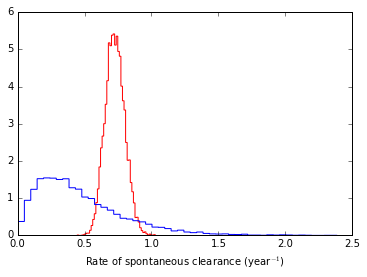
\includegraphics[width=10cm]{england_files/england_14_1.png}\end{center}
        \caption{Sampled rates of spontaneous chlamydia clearance in men (blue) and women (red).}
        \label{fig:sc_samples}
    \end{figure}
    
    \subsubsection{Proportion of incident infections
asymptomatic}\label{proportion-of-incident-infections-asymptomatic}

Finally, we infer the proportion of infections which are asymptomatic by
calibrating to the Natsal-3 prevalence estimates in 16-25-year-old men
and women.

    \begin{footnotesize}
        \begin{Verbatim}[commandchars=\\\{\}]
{\color{incolor}In [{\color{incolor}10}]:} \PY{k+kn}{from} \PY{n+nn}{scipy.stats} \PY{k+kn}{import} \PY{n}{beta}
         
         \PY{p}{[}\PY{n}{alpha\PYZus{}prev\PYZus{}m}\PY{p}{,} \PY{n}{beta\PYZus{}prev\PYZus{}m}\PY{p}{]} \PY{o}{=} \PY{n}{fsolve}\PY{p}{(}
             \PY{k}{lambda} \PY{n}{x}\PY{p}{:} \PY{n}{array}\PY{p}{(}\PY{n}{beta}\PY{o}{.}\PY{n}{interval}\PY{p}{(}\PY{l+m+mf}{0.95}\PY{p}{,} \PY{n}{x}\PY{p}{[}\PY{l+m+mi}{0}\PY{p}{]}\PY{p}{,} \PY{n}{x}\PY{p}{[}\PY{l+m+mi}{1}\PY{p}{]}\PY{p}{,} \PY{n}{loc}\PY{o}{=}\PY{l+m+mi}{0}\PY{p}{,} \PY{n}{scale}\PY{o}{=}\PY{l+m+mi}{1}\PY{p}{)}\PY{p}{)}
             \PY{o}{\PYZhy{}} \PY{p}{(}\PY{l+m+mf}{0.015}\PY{p}{,} \PY{l+m+mf}{0.034}\PY{p}{)}\PY{p}{,} \PY{c}{\PYZsh{} Natsal\PYZhy{}3 prevalence in men}
             \PY{p}{[}\PY{l+m+mi}{1}\PY{p}{,}\PY{l+m+mi}{1}\PY{p}{]}
             \PY{p}{)}
         
         \PY{n}{prev\PYZus{}m} \PY{o}{=} \PY{n}{rs}\PY{o}{.}\PY{n}{beta}\PY{p}{(}\PY{n}{alpha\PYZus{}prev\PYZus{}m}\PY{p}{,} \PY{n}{beta\PYZus{}prev\PYZus{}m}\PY{p}{,} \PY{n}{size}\PY{o}{=}\PY{n}{n\PYZus{}sample}\PY{p}{)}
         
         \PY{c}{\PYZsh{} generate samples for prevalence}
         \PY{p}{[}\PY{n}{alpha\PYZus{}prev\PYZus{}f}\PY{p}{,} \PY{n}{beta\PYZus{}prev\PYZus{}f}\PY{p}{]} \PY{o}{=} \PY{n}{fsolve}\PY{p}{(}
             \PY{k}{lambda} \PY{n}{x}\PY{p}{:} \PY{n}{array}\PY{p}{(}\PY{n}{beta}\PY{o}{.}\PY{n}{interval}\PY{p}{(}\PY{l+m+mf}{0.95}\PY{p}{,} \PY{n}{x}\PY{p}{[}\PY{l+m+mi}{0}\PY{p}{]}\PY{p}{,} \PY{n}{x}\PY{p}{[}\PY{l+m+mi}{1}\PY{p}{]}\PY{p}{,} \PY{n}{loc}\PY{o}{=}\PY{l+m+mi}{0}\PY{p}{,} \PY{n}{scale}\PY{o}{=}\PY{l+m+mi}{1}\PY{p}{)}\PY{p}{)}
             \PY{o}{\PYZhy{}} \PY{p}{(}\PY{l+m+mf}{0.022}\PY{p}{,} \PY{l+m+mf}{0.043}\PY{p}{)}\PY{p}{,} \PY{c}{\PYZsh{} Natsal\PYZhy{}3 prevalence in women}
             \PY{p}{[}\PY{l+m+mi}{1}\PY{p}{,}\PY{l+m+mi}{1}\PY{p}{]}
             \PY{p}{)}
         
         \PY{n}{prev\PYZus{}f} \PY{o}{=} \PY{n}{rs}\PY{o}{.}\PY{n}{beta}\PY{p}{(}\PY{n}{alpha\PYZus{}prev\PYZus{}f}\PY{p}{,} \PY{n}{beta\PYZus{}prev\PYZus{}f}\PY{p}{,} \PY{n}{size}\PY{o}{=}\PY{n}{n\PYZus{}sample}\PY{p}{)}
\end{Verbatim}
    \end{footnotesize}

    \begin{footnotesize}
        \begin{Verbatim}[commandchars=\\\{\}]
{\color{incolor}In [{\color{incolor}11}]:} \PY{c}{\PYZsh{} This script also contains the functions linking observed tests, symptomatic/asymptomatic/toal diagnoses, }
         \PY{c}{\PYZsh{} incidence, prevalence, screening and other model parameters}
         \PY{c}{\PYZsh{} Running it takes a little while because of all the symbolic algebra}
         \PY{o}{\PYZpc{}}\PY{k}{run} test\PYZus{}diag\PYZus{}fun.py
\end{Verbatim}
    \end{footnotesize}

    \begin{footnotesize}
        \begin{Verbatim}[commandchars=\\\{\}]
{\color{incolor}In [{\color{incolor}12}]:} \PY{c}{\PYZsh{} incidence, screening and proportion of incident infections asymptomatic in men}
         
         \PY{n}{inc\PYZus{}m} \PY{o}{=} \PY{n}{np}\PY{o}{.}\PY{n}{zeros}\PY{p}{(}\PY{n}{n\PYZus{}sample}\PY{p}{)}
         \PY{n}{scr\PYZus{}m} \PY{o}{=} \PY{n}{np}\PY{o}{.}\PY{n}{zeros}\PY{p}{(}\PY{n}{n\PYZus{}sample}\PY{p}{)}
         \PY{n}{p\PYZus{}asymp\PYZus{}m} \PY{o}{=} \PY{n}{np}\PY{o}{.}\PY{n}{zeros}\PY{p}{(}\PY{n}{n\PYZus{}sample}\PY{p}{)}
         
         \PY{k}{for} \PY{n}{i} \PY{o+ow}{in} \PY{n+nb}{xrange}\PY{p}{(}\PY{n}{n\PYZus{}sample}\PY{p}{)}\PY{p}{:}
             \PY{k}{def} \PY{n+nf}{tmpfun}\PY{p}{(}\PY{n}{inc}\PY{p}{,} \PY{n}{scr}\PY{p}{,} \PY{n}{p\PYZus{}asymp}\PY{p}{)}\PY{p}{:}
                 \PY{p}{[}\PY{n}{tr}\PY{p}{,} \PY{n}{dr}\PY{p}{]} \PY{o}{=} \PY{n}{test\PYZus{}diag\PYZus{}fun}\PY{p}{(}
                     \PY{n}{array}\PY{p}{(}\PY{p}{[}
                         \PY{n}{inc}\PY{p}{,}
                         \PY{n}{scr}\PY{p}{,}
                         \PY{l+m+mi}{1}\PY{o}{\PYZhy{}}\PY{n}{p\PYZus{}asymp}\PY{p}{,} \PY{c}{\PYZsh{} proportion of incident infections which are symptomatic}
                         \PY{n}{sc\PYZus{}m}\PY{p}{[}\PY{n}{i}\PY{p}{]}\PY{p}{,} \PY{c}{\PYZsh{} rate of self\PYZhy{}clear }
                         \PY{n}{att\PYZus{}symp}\PY{p}{[}\PY{n}{i}\PY{p}{]}\PY{p}{,}
                         \PY{n}{p\PYZus{}true\PYZus{}pos\PYZus{}m}\PY{p}{[}\PY{n}{i}\PY{p}{]}\PY{p}{,} 
                         \PY{n}{p\PYZus{}false\PYZus{}pos\PYZus{}m}\PY{p}{[}\PY{n}{i}\PY{p}{]}
                         \PY{p}{]}\PY{p}{)}\PY{p}{)}
                 \PY{n}{prev} \PY{o}{=} \PY{n}{dyn\PYZus{}fun}\PY{p}{(}
                     \PY{n}{inc}\PY{o}{*}\PY{n}{p\PYZus{}asymp}\PY{p}{,} 
                     \PY{n}{sc\PYZus{}m}\PY{p}{[}\PY{n}{i}\PY{p}{]} \PY{o}{+} \PY{n}{scr}\PY{o}{*}\PY{n}{p\PYZus{}true\PYZus{}pos\PYZus{}m}\PY{p}{[}\PY{n}{i}\PY{p}{]}\PY{p}{,} 
                     \PY{n}{inc}\PY{o}{*}\PY{p}{(}\PY{l+m+mi}{1}\PY{o}{\PYZhy{}}\PY{n}{p\PYZus{}asymp}\PY{p}{)}\PY{p}{,} 
                     \PY{n}{scr}\PY{o}{*}\PY{n}{p\PYZus{}true\PYZus{}pos\PYZus{}m}\PY{p}{[}\PY{n}{i}\PY{p}{]} \PY{o}{+} \PY{n}{att\PYZus{}symp}\PY{p}{[}\PY{n}{i}\PY{p}{]}\PY{o}{*}\PY{n}{p\PYZus{}true\PYZus{}pos\PYZus{}m}\PY{p}{[}\PY{n}{i}\PY{p}{]}
                 \PY{p}{)} 
                 \PY{k}{return} \PY{p}{(}\PY{n}{tr} \PY{o}{\PYZhy{}} \PY{n}{test\PYZus{}rate\PYZus{}m\PYZus{}15\PYZus{}24}\PY{p}{[}\PY{n}{i}\PY{p}{]}\PY{p}{,} 
                         \PY{n}{dr} \PY{o}{\PYZhy{}} \PY{n}{diag\PYZus{}rate\PYZus{}m\PYZus{}15\PYZus{}24}\PY{p}{[}\PY{n}{i}\PY{p}{]}\PY{p}{,} 
                         \PY{n}{prev} \PY{o}{\PYZhy{}} \PY{n}{prev\PYZus{}m}\PY{p}{[}\PY{n}{i}\PY{p}{]}\PY{p}{)}
         
             \PY{p}{[}\PY{n}{inc\PYZus{}m}\PY{p}{[}\PY{n}{i}\PY{p}{]}\PY{p}{,} \PY{n}{scr\PYZus{}m}\PY{p}{[}\PY{n}{i}\PY{p}{]}\PY{p}{,} \PY{n}{p\PYZus{}asymp\PYZus{}m}\PY{p}{[}\PY{n}{i}\PY{p}{]}\PY{p}{]} \PY{o}{=} \PY{n}{fsolve}\PY{p}{(}\PY{k}{lambda} \PY{n}{x}\PY{p}{:} \PY{n}{tmpfun}\PY{p}{(}\PY{n}{x}\PY{p}{[}\PY{l+m+mi}{0}\PY{p}{]}\PY{p}{,} \PY{n}{x}\PY{p}{[}\PY{l+m+mi}{1}\PY{p}{]}\PY{p}{,} \PY{n}{x}\PY{p}{[}\PY{l+m+mi}{2}\PY{p}{]}\PY{p}{)}\PY{p}{,} \PY{p}{[}\PY{l+m+mf}{0.09}\PY{p}{,} \PY{l+m+mf}{0.25}\PY{p}{,} \PY{l+m+mf}{0.9}\PY{p}{]} \PY{p}{)}
\end{Verbatim}
    \end{footnotesize}

    \begin{footnotesize}
        \begin{Verbatim}[commandchars=\\\{\}]
{\color{incolor}In [{\color{incolor}13}]:} \PY{c}{\PYZsh{} Figure 3}
         \PY{c}{\PYZsh{} incidence, screening and proportion of incident infections asymptomatic in women}
         
         \PY{n}{inc\PYZus{}f} \PY{o}{=} \PY{n}{np}\PY{o}{.}\PY{n}{zeros}\PY{p}{(}\PY{n}{n\PYZus{}sample}\PY{p}{)}
         \PY{n}{scr\PYZus{}f} \PY{o}{=} \PY{n}{np}\PY{o}{.}\PY{n}{zeros}\PY{p}{(}\PY{n}{n\PYZus{}sample}\PY{p}{)}
         \PY{n}{p\PYZus{}asymp\PYZus{}f} \PY{o}{=} \PY{n}{np}\PY{o}{.}\PY{n}{zeros}\PY{p}{(}\PY{n}{n\PYZus{}sample}\PY{p}{)}
         
         \PY{k}{for} \PY{n}{i} \PY{o+ow}{in} \PY{n+nb}{xrange}\PY{p}{(}\PY{n}{n\PYZus{}sample}\PY{p}{)}\PY{p}{:}
             \PY{k}{def} \PY{n+nf}{tmpfun}\PY{p}{(}\PY{n}{inc}\PY{p}{,} \PY{n}{scr}\PY{p}{,} \PY{n}{p\PYZus{}asymp}\PY{p}{)}\PY{p}{:}
                 \PY{p}{[}\PY{n}{tr}\PY{p}{,} \PY{n}{dr}\PY{p}{]} \PY{o}{=} \PY{n}{test\PYZus{}diag\PYZus{}fun}\PY{p}{(}
                     \PY{n}{array}\PY{p}{(}\PY{p}{[}
                         \PY{n}{inc}\PY{p}{,}
                         \PY{n}{scr}\PY{p}{,}
                         \PY{l+m+mi}{1}\PY{o}{\PYZhy{}}\PY{n}{p\PYZus{}asymp}\PY{p}{,} \PY{c}{\PYZsh{} proportion of incident infections which are symptomatic}
                         \PY{n}{sc\PYZus{}f}\PY{p}{[}\PY{n}{i}\PY{p}{]}\PY{p}{,} \PY{c}{\PYZsh{} rate of self\PYZhy{}clear }
                         \PY{n}{att\PYZus{}symp}\PY{p}{[}\PY{n}{i}\PY{p}{]}\PY{p}{,}
                         \PY{n}{p\PYZus{}true\PYZus{}pos\PYZus{}f}\PY{p}{[}\PY{n}{i}\PY{p}{]}\PY{p}{,} 
                         \PY{n}{p\PYZus{}false\PYZus{}pos\PYZus{}f}\PY{p}{[}\PY{n}{i}\PY{p}{]}
                         \PY{p}{]}\PY{p}{)}\PY{p}{)}
                 \PY{n}{prev} \PY{o}{=} \PY{n}{dyn\PYZus{}fun}\PY{p}{(}
                     \PY{n}{inc}\PY{o}{*}\PY{n}{p\PYZus{}asymp}\PY{p}{,} 
                     \PY{n}{sc\PYZus{}f}\PY{p}{[}\PY{n}{i}\PY{p}{]} \PY{o}{+} \PY{n}{scr}\PY{o}{*}\PY{n}{p\PYZus{}true\PYZus{}pos\PYZus{}f}\PY{p}{[}\PY{n}{i}\PY{p}{]}\PY{p}{,} 
                     \PY{n}{inc}\PY{o}{*}\PY{p}{(}\PY{l+m+mi}{1}\PY{o}{\PYZhy{}}\PY{n}{p\PYZus{}asymp}\PY{p}{)}\PY{p}{,} 
                     \PY{n}{scr}\PY{o}{*}\PY{n}{p\PYZus{}true\PYZus{}pos\PYZus{}f}\PY{p}{[}\PY{n}{i}\PY{p}{]} \PY{o}{+} \PY{n}{att\PYZus{}symp}\PY{p}{[}\PY{n}{i}\PY{p}{]}\PY{o}{*}\PY{n}{p\PYZus{}true\PYZus{}pos\PYZus{}f}\PY{p}{[}\PY{n}{i}\PY{p}{]}
                 \PY{p}{)} 
                 \PY{k}{return} \PY{p}{(}\PY{n}{tr} \PY{o}{\PYZhy{}} \PY{n}{test\PYZus{}rate\PYZus{}f\PYZus{}15\PYZus{}24}\PY{p}{[}\PY{n}{i}\PY{p}{]}\PY{p}{,} 
                         \PY{n}{dr} \PY{o}{\PYZhy{}} \PY{n}{diag\PYZus{}rate\PYZus{}f\PYZus{}15\PYZus{}24}\PY{p}{[}\PY{n}{i}\PY{p}{]}\PY{p}{,} 
                         \PY{n}{prev} \PY{o}{\PYZhy{}} \PY{n}{prev\PYZus{}f}\PY{p}{[}\PY{n}{i}\PY{p}{]}\PY{p}{)}
         
             \PY{p}{[}\PY{n}{inc\PYZus{}f}\PY{p}{[}\PY{n}{i}\PY{p}{]}\PY{p}{,} \PY{n}{scr\PYZus{}f}\PY{p}{[}\PY{n}{i}\PY{p}{]}\PY{p}{,} \PY{n}{p\PYZus{}asymp\PYZus{}f}\PY{p}{[}\PY{n}{i}\PY{p}{]}\PY{p}{]} \PY{o}{=} \PY{n}{fsolve}\PY{p}{(}\PY{k}{lambda} \PY{n}{x}\PY{p}{:} \PY{n}{tmpfun}\PY{p}{(}\PY{n}{x}\PY{p}{[}\PY{l+m+mi}{0}\PY{p}{]}\PY{p}{,} \PY{n}{x}\PY{p}{[}\PY{l+m+mi}{1}\PY{p}{]}\PY{p}{,} \PY{n}{x}\PY{p}{[}\PY{l+m+mi}{2}\PY{p}{]}\PY{p}{)}\PY{p}{,} \PY{p}{[}\PY{l+m+mf}{0.09}\PY{p}{,} \PY{l+m+mf}{0.25}\PY{p}{,} \PY{l+m+mf}{0.9}\PY{p}{]} \PY{p}{)}
\end{Verbatim}
    \end{footnotesize}

    \begin{footnotesize}
        \begin{Verbatim}[commandchars=\\\{\}]
{\color{incolor}In [{\color{incolor}14}]:} \PY{n}{h}\PY{o}{=}\PY{n}{plt}\PY{o}{.}\PY{n}{hist}\PY{p}{(}\PY{n}{p\PYZus{}asymp\PYZus{}f}\PY{p}{,} \PY{n}{bins}\PY{o}{=}\PY{l+m+mi}{50}\PY{p}{,} \PY{n}{histtype}\PY{o}{=}\PY{l+s}{\PYZsq{}}\PY{l+s}{step}\PY{l+s}{\PYZsq{}}\PY{p}{,} \PY{n}{normed}\PY{o}{=}\PY{n+nb+bp}{True}\PY{p}{,} \PY{n}{color}\PY{o}{=}\PY{l+s}{\PYZsq{}}\PY{l+s}{r}\PY{l+s}{\PYZsq{}}\PY{p}{)}
         \PY{n}{h}\PY{o}{=}\PY{n}{plt}\PY{o}{.}\PY{n}{hist}\PY{p}{(}\PY{n}{p\PYZus{}asymp\PYZus{}m}\PY{p}{,} \PY{n}{bins}\PY{o}{=}\PY{l+m+mi}{50}\PY{p}{,} \PY{n}{histtype}\PY{o}{=}\PY{l+s}{\PYZsq{}}\PY{l+s}{step}\PY{l+s}{\PYZsq{}}\PY{p}{,} \PY{n}{normed}\PY{o}{=}\PY{n+nb+bp}{True}\PY{p}{,} \PY{n}{color}\PY{o}{=}\PY{l+s}{\PYZsq{}}\PY{l+s}{b}\PY{l+s}{\PYZsq{}}\PY{p}{)}
         \PY{n}{plt}\PY{o}{.}\PY{n}{xlabel}\PY{p}{(}\PY{l+s}{\PYZsq{}}\PY{l+s}{Proportion of incident infections which are asymptomatic}\PY{l+s}{\PYZsq{}}\PY{p}{)}
         
         \PY{k}{print} \PY{l+s}{\PYZsq{}}\PY{l+s}{Mean proportion asymptomatic in men:}\PY{l+s}{\PYZsq{}}\PY{p}{,} \PY{n}{mean}\PY{p}{(}\PY{n}{p\PYZus{}asymp\PYZus{}m}\PY{p}{)}
         \PY{k}{print} \PY{l+s}{\PYZsq{}}\PY{l+s}{Median (central 95}\PY{l+s+si}{\PYZpc{} c}\PY{l+s}{redible interval) for proportion asymptomatic in men: }\PY{l+s+se}{\PYZbs{}n}\PY{l+s}{ }\PY{l+s+se}{\PYZbs{}t}\PY{l+s}{\PYZsq{}}\PY{p}{,} \PYZbs{}
             \PY{n}{percentile}\PY{p}{(}\PY{n}{p\PYZus{}asymp\PYZus{}m}\PY{p}{,} \PY{l+m+mi}{50}\PY{p}{)}\PY{p}{,} \PY{n}{percentile}\PY{p}{(}\PY{n}{p\PYZus{}asymp\PYZus{}m}\PY{p}{,} \PY{p}{(}\PY{l+m+mf}{2.5}\PY{p}{,}\PY{l+m+mf}{97.5}\PY{p}{)}\PY{p}{)}
         \PY{k}{print} \PY{l+s}{\PYZsq{}}\PY{l+s}{Mean proportion asymptomatic in women:}\PY{l+s}{\PYZsq{}}\PY{p}{,} \PY{n}{mean}\PY{p}{(}\PY{n}{p\PYZus{}asymp\PYZus{}f}\PY{p}{)}
         \PY{k}{print} \PY{l+s}{\PYZsq{}}\PY{l+s}{Median (central 95}\PY{l+s+si}{\PYZpc{} c}\PY{l+s}{redible interval) for proportion asymptomatic in women:}\PY{l+s+se}{\PYZbs{}n}\PY{l+s}{ }\PY{l+s+se}{\PYZbs{}t}\PY{l+s}{\PYZsq{}}\PY{p}{,} \PYZbs{}
             \PY{n}{percentile}\PY{p}{(}\PY{n}{p\PYZus{}asymp\PYZus{}f}\PY{p}{,} \PY{l+m+mi}{50}\PY{p}{)}\PY{p}{,} \PY{n}{percentile}\PY{p}{(}\PY{n}{p\PYZus{}asymp\PYZus{}f}\PY{p}{,} \PY{p}{(}\PY{l+m+mf}{2.5}\PY{p}{,}\PY{l+m+mf}{97.5}\PY{p}{)}\PY{p}{)}
\end{Verbatim}
    \end{footnotesize}

    \begin{Verbatim}[commandchars=\\\{\}]
Mean proportion asymptomatic in men: 0.510862240434
Median (central 95\% credible interval) for proportion asymptomatic in men: 
 	0.509889142897 [0.26393408139570879, 0.75872661515902395]
Mean proportion asymptomatic in women: 0.615291469484
Median (central 95\% credible interval) for proportion asymptomatic in women:
 	0.616465413009 [0.46763845173602908, 0.75205517865264992]
    \end{Verbatim}

    \begin{figure}
        \begin{center}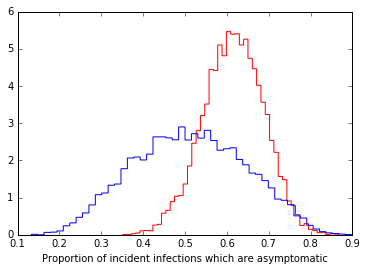
\includegraphics[width=10cm]{england_files/england_20_1.png}\end{center}
        \caption{Samples for the proportion of incident infections which are asymptomatic in men (blue) and women (red), calibrated to Natsal-3 prevalence estimates in 16-24-year-olds.}
        \label{fig:p_asymp_samples}
    \end{figure}
    
    \subsection{Estimating national
prevalence}\label{estimating-national-prevalence}

The sampled parameter values are now used to infer prevalence in men and
women in different age groups.

    \begin{footnotesize}
        \begin{Verbatim}[commandchars=\\\{\}]
{\color{incolor}In [{\color{incolor}15}]:} \PY{k+kn}{from} \PY{n+nn}{scipy.optimize} \PY{k+kn}{import} \PY{n}{fsolve}
\end{Verbatim}
    \end{footnotesize}

    \begin{footnotesize}
        \begin{Verbatim}[commandchars=\\\{\}]
{\color{incolor}In [{\color{incolor}16}]:} \PY{c}{\PYZsh{} men first...}
         \PY{n}{prev\PYZus{}m\PYZus{}15\PYZus{}19} \PY{o}{=} \PY{n}{np}\PY{o}{.}\PY{n}{zeros}\PY{p}{(}\PY{n}{n\PYZus{}sample}\PY{p}{)}
         \PY{n}{inc\PYZus{}m\PYZus{}15\PYZus{}19} \PY{o}{=} \PY{n}{np}\PY{o}{.}\PY{n}{zeros}\PY{p}{(}\PY{n}{n\PYZus{}sample}\PY{p}{)}
         \PY{n}{scr\PYZus{}m\PYZus{}15\PYZus{}19} \PY{o}{=} \PY{n}{np}\PY{o}{.}\PY{n}{zeros}\PY{p}{(}\PY{n}{n\PYZus{}sample}\PY{p}{)}
         
         \PY{k}{for} \PY{n}{i} \PY{o+ow}{in} \PY{n+nb}{xrange}\PY{p}{(}\PY{n}{n\PYZus{}sample}\PY{p}{)}\PY{p}{:}
             \PY{p}{[}\PY{n}{inc\PYZus{}m\PYZus{}15\PYZus{}19}\PY{p}{[}\PY{n}{i}\PY{p}{]}\PY{p}{,} \PY{n}{scr\PYZus{}m\PYZus{}15\PYZus{}19}\PY{p}{[}\PY{n}{i}\PY{p}{]}\PY{p}{]} \PY{o}{=} \PY{n}{fsolve}\PY{p}{(}\PY{k}{lambda} \PY{n}{x}\PY{p}{:} \PY{n}{test\PYZus{}diag\PYZus{}fun}\PY{p}{(}\PY{n}{concatenate}\PY{p}{(}\PY{p}{[}
                             \PY{n}{x}\PY{p}{,} \PY{n}{array}\PY{p}{(}\PY{p}{[}
                                     \PY{l+m+mi}{1}\PY{o}{\PYZhy{}}\PY{n}{p\PYZus{}asymp\PYZus{}m}\PY{p}{[}\PY{n}{i}\PY{p}{]}\PY{p}{,} \PY{c}{\PYZsh{} proportion of incident infections which are symptomatic}
                                     \PY{n}{sc\PYZus{}m}\PY{p}{[}\PY{n}{i}\PY{p}{]}\PY{p}{,} \PY{c}{\PYZsh{} rate of self\PYZhy{}clear }
                                     \PY{n}{att\PYZus{}symp}\PY{p}{[}\PY{n}{i}\PY{p}{]}\PY{p}{,}
                                     \PY{n}{p\PYZus{}true\PYZus{}pos\PYZus{}m}\PY{p}{[}\PY{n}{i}\PY{p}{]}\PY{p}{,} 
                                     \PY{n}{p\PYZus{}false\PYZus{}pos\PYZus{}m}\PY{p}{[}\PY{n}{i}\PY{p}{]}
                                 \PY{p}{]}\PY{p}{)}\PY{p}{]}\PY{p}{)}\PY{p}{)} \PY{o}{\PYZhy{}} \PY{n}{array}\PY{p}{(}\PY{p}{[}\PY{n}{test\PYZus{}rate\PYZus{}m\PYZus{}15\PYZus{}19}\PY{p}{[}\PY{n}{i}\PY{p}{]}\PY{p}{,}\PY{n}{diag\PYZus{}rate\PYZus{}m\PYZus{}15\PYZus{}19}\PY{p}{[}\PY{n}{i}\PY{p}{]}\PY{p}{]}\PY{p}{)}\PY{p}{,} \PY{p}{[}\PY{l+m+mf}{0.09}\PY{p}{,} \PY{l+m+mf}{0.25}\PY{p}{]}\PY{p}{)}
             \PY{n}{prev\PYZus{}m\PYZus{}15\PYZus{}19}\PY{p}{[}\PY{n}{i}\PY{p}{]} \PY{o}{=} \PY{n}{dyn\PYZus{}fun}\PY{p}{(}
                 \PY{n}{inc\PYZus{}m\PYZus{}15\PYZus{}19}\PY{p}{[}\PY{n}{i}\PY{p}{]}\PY{o}{*}\PY{n}{p\PYZus{}asymp\PYZus{}m}\PY{p}{[}\PY{n}{i}\PY{p}{]}\PY{p}{,} 
                 \PY{n}{sc\PYZus{}m}\PY{p}{[}\PY{n}{i}\PY{p}{]} \PY{o}{+} \PY{n}{scr\PYZus{}m\PYZus{}15\PYZus{}19}\PY{p}{[}\PY{n}{i}\PY{p}{]}\PY{o}{*}\PY{n}{p\PYZus{}true\PYZus{}pos\PYZus{}m}\PY{p}{[}\PY{n}{i}\PY{p}{]}\PY{p}{,} 
                 \PY{n}{inc\PYZus{}m\PYZus{}15\PYZus{}19}\PY{p}{[}\PY{n}{i}\PY{p}{]}\PY{o}{*}\PY{p}{(}\PY{l+m+mi}{1}\PY{o}{\PYZhy{}}\PY{n}{p\PYZus{}asymp\PYZus{}m}\PY{p}{[}\PY{n}{i}\PY{p}{]}\PY{p}{)}\PY{p}{,} 
                 \PY{n}{scr\PYZus{}m\PYZus{}15\PYZus{}19}\PY{p}{[}\PY{n}{i}\PY{p}{]}\PY{o}{*}\PY{n}{p\PYZus{}true\PYZus{}pos\PYZus{}m}\PY{p}{[}\PY{n}{i}\PY{p}{]} \PY{o}{+} \PY{n}{att\PYZus{}symp}\PY{p}{[}\PY{n}{i}\PY{p}{]}\PY{o}{*}\PY{n}{p\PYZus{}true\PYZus{}pos\PYZus{}m}\PY{p}{[}\PY{n}{i}\PY{p}{]}
             \PY{p}{)}
\end{Verbatim}
    \end{footnotesize}

    \begin{footnotesize}
        \begin{Verbatim}[commandchars=\\\{\}]
{\color{incolor}In [{\color{incolor}17}]:} \PY{n}{prev\PYZus{}m\PYZus{}20\PYZus{}24} \PY{o}{=} \PY{n}{np}\PY{o}{.}\PY{n}{zeros}\PY{p}{(}\PY{n}{n\PYZus{}sample}\PY{p}{)}
         \PY{n}{inc\PYZus{}m\PYZus{}20\PYZus{}24} \PY{o}{=} \PY{n}{np}\PY{o}{.}\PY{n}{zeros}\PY{p}{(}\PY{n}{n\PYZus{}sample}\PY{p}{)}
         \PY{n}{scr\PYZus{}m\PYZus{}20\PYZus{}24} \PY{o}{=} \PY{n}{np}\PY{o}{.}\PY{n}{zeros}\PY{p}{(}\PY{n}{n\PYZus{}sample}\PY{p}{)}
         
         \PY{k}{for} \PY{n}{i} \PY{o+ow}{in} \PY{n+nb}{xrange}\PY{p}{(}\PY{n}{n\PYZus{}sample}\PY{p}{)}\PY{p}{:}
             \PY{p}{[}\PY{n}{inc\PYZus{}m\PYZus{}20\PYZus{}24}\PY{p}{[}\PY{n}{i}\PY{p}{]}\PY{p}{,} \PY{n}{scr\PYZus{}m\PYZus{}20\PYZus{}24}\PY{p}{[}\PY{n}{i}\PY{p}{]}\PY{p}{]} \PY{o}{=} \PY{n}{fsolve}\PY{p}{(}\PY{k}{lambda} \PY{n}{x}\PY{p}{:} \PY{n}{test\PYZus{}diag\PYZus{}fun}\PY{p}{(}\PY{n}{concatenate}\PY{p}{(}\PY{p}{[}
                             \PY{n}{x}\PY{p}{,} \PY{n}{array}\PY{p}{(}\PY{p}{[}
                                     \PY{l+m+mi}{1}\PY{o}{\PYZhy{}}\PY{n}{p\PYZus{}asymp\PYZus{}m}\PY{p}{[}\PY{n}{i}\PY{p}{]}\PY{p}{,} \PY{c}{\PYZsh{} proportion of incident infections which are symptomatic}
                                     \PY{n}{sc\PYZus{}m}\PY{p}{[}\PY{n}{i}\PY{p}{]}\PY{p}{,} \PY{c}{\PYZsh{} rate of self\PYZhy{}clear }
                                     \PY{n}{att\PYZus{}symp}\PY{p}{[}\PY{n}{i}\PY{p}{]}\PY{p}{,}
                                     \PY{n}{p\PYZus{}true\PYZus{}pos\PYZus{}m}\PY{p}{[}\PY{n}{i}\PY{p}{]}\PY{p}{,} 
                                     \PY{n}{p\PYZus{}false\PYZus{}pos\PYZus{}m}\PY{p}{[}\PY{n}{i}\PY{p}{]}
                                 \PY{p}{]}\PY{p}{)}\PY{p}{]}\PY{p}{)}\PY{p}{)} \PY{o}{\PYZhy{}} \PY{n}{array}\PY{p}{(}\PY{p}{[}\PY{n}{test\PYZus{}rate\PYZus{}m\PYZus{}20\PYZus{}24}\PY{p}{[}\PY{n}{i}\PY{p}{]}\PY{p}{,}\PY{n}{diag\PYZus{}rate\PYZus{}m\PYZus{}20\PYZus{}24}\PY{p}{[}\PY{n}{i}\PY{p}{]}\PY{p}{]}\PY{p}{)}\PY{p}{,} \PY{p}{[}\PY{l+m+mf}{0.09}\PY{p}{,} \PY{l+m+mf}{0.25}\PY{p}{]}\PY{p}{)}
             \PY{n}{prev\PYZus{}m\PYZus{}20\PYZus{}24}\PY{p}{[}\PY{n}{i}\PY{p}{]} \PY{o}{=} \PY{n}{dyn\PYZus{}fun}\PY{p}{(}
                 \PY{n}{inc\PYZus{}m\PYZus{}20\PYZus{}24}\PY{p}{[}\PY{n}{i}\PY{p}{]}\PY{o}{*}\PY{n}{p\PYZus{}asymp\PYZus{}m}\PY{p}{[}\PY{n}{i}\PY{p}{]}\PY{p}{,} 
                 \PY{n}{sc\PYZus{}m}\PY{p}{[}\PY{n}{i}\PY{p}{]} \PY{o}{+} \PY{n}{scr\PYZus{}m\PYZus{}20\PYZus{}24}\PY{p}{[}\PY{n}{i}\PY{p}{]}\PY{o}{*}\PY{n}{p\PYZus{}true\PYZus{}pos\PYZus{}m}\PY{p}{[}\PY{n}{i}\PY{p}{]}\PY{p}{,} 
                 \PY{n}{inc\PYZus{}m\PYZus{}20\PYZus{}24}\PY{p}{[}\PY{n}{i}\PY{p}{]}\PY{o}{*}\PY{p}{(}\PY{l+m+mi}{1}\PY{o}{\PYZhy{}}\PY{n}{p\PYZus{}asymp\PYZus{}m}\PY{p}{[}\PY{n}{i}\PY{p}{]}\PY{p}{)}\PY{p}{,} 
                 \PY{n}{att\PYZus{}symp}\PY{p}{[}\PY{n}{i}\PY{p}{]}\PY{o}{*}\PY{n}{p\PYZus{}true\PYZus{}pos\PYZus{}m}\PY{p}{[}\PY{n}{i}\PY{p}{]}
             \PY{p}{)}
\end{Verbatim}
    \end{footnotesize}

    \begin{footnotesize}
        \begin{Verbatim}[commandchars=\\\{\}]
{\color{incolor}In [{\color{incolor}18}]:} \PY{c}{\PYZsh{} ... then women}
         \PY{n}{prev\PYZus{}f\PYZus{}15\PYZus{}19} \PY{o}{=} \PY{n}{np}\PY{o}{.}\PY{n}{zeros}\PY{p}{(}\PY{n}{n\PYZus{}sample}\PY{p}{)}
         \PY{n}{inc\PYZus{}f\PYZus{}15\PYZus{}19} \PY{o}{=} \PY{n}{np}\PY{o}{.}\PY{n}{zeros}\PY{p}{(}\PY{n}{n\PYZus{}sample}\PY{p}{)}
         \PY{n}{scr\PYZus{}f\PYZus{}15\PYZus{}19} \PY{o}{=} \PY{n}{np}\PY{o}{.}\PY{n}{zeros}\PY{p}{(}\PY{n}{n\PYZus{}sample}\PY{p}{)}
         
         \PY{k}{for} \PY{n}{i} \PY{o+ow}{in} \PY{n+nb}{xrange}\PY{p}{(}\PY{n}{n\PYZus{}sample}\PY{p}{)}\PY{p}{:}
             \PY{p}{[}\PY{n}{inc\PYZus{}f\PYZus{}15\PYZus{}19}\PY{p}{[}\PY{n}{i}\PY{p}{]}\PY{p}{,} \PY{n}{scr\PYZus{}f\PYZus{}15\PYZus{}19}\PY{p}{[}\PY{n}{i}\PY{p}{]}\PY{p}{]} \PY{o}{=} \PY{n}{fsolve}\PY{p}{(}\PY{k}{lambda} \PY{n}{x}\PY{p}{:} \PY{n}{test\PYZus{}diag\PYZus{}fun}\PY{p}{(}\PY{n}{concatenate}\PY{p}{(}\PY{p}{[}
                             \PY{n}{x}\PY{p}{,} \PY{n}{array}\PY{p}{(}\PY{p}{[}
                                     \PY{l+m+mi}{1}\PY{o}{\PYZhy{}}\PY{n}{p\PYZus{}asymp\PYZus{}f}\PY{p}{[}\PY{n}{i}\PY{p}{]}\PY{p}{,} \PY{c}{\PYZsh{} proportion of incident infections which are symptomatic}
                                     \PY{n}{sc\PYZus{}f}\PY{p}{[}\PY{n}{i}\PY{p}{]}\PY{p}{,} \PY{c}{\PYZsh{} rate of self\PYZhy{}clear }
                                     \PY{n}{att\PYZus{}symp}\PY{p}{[}\PY{n}{i}\PY{p}{]}\PY{p}{,}
                                     \PY{n}{p\PYZus{}true\PYZus{}pos\PYZus{}f}\PY{p}{[}\PY{n}{i}\PY{p}{]}\PY{p}{,} 
                                     \PY{n}{p\PYZus{}false\PYZus{}pos\PYZus{}f}\PY{p}{[}\PY{n}{i}\PY{p}{]}
                                 \PY{p}{]}\PY{p}{)}\PY{p}{]}\PY{p}{)}\PY{p}{)} \PY{o}{\PYZhy{}} \PY{n}{array}\PY{p}{(}\PY{p}{[}\PY{n}{test\PYZus{}rate\PYZus{}f\PYZus{}15\PYZus{}19}\PY{p}{[}\PY{n}{i}\PY{p}{]}\PY{p}{,}\PY{n}{diag\PYZus{}rate\PYZus{}f\PYZus{}15\PYZus{}19}\PY{p}{[}\PY{n}{i}\PY{p}{]}\PY{p}{]}\PY{p}{)}\PY{p}{,} \PY{p}{[}\PY{l+m+mf}{0.03}\PY{p}{,} \PY{l+m+mf}{0.44}\PY{p}{]}\PY{p}{)}
             \PY{n}{prev\PYZus{}f\PYZus{}15\PYZus{}19}\PY{p}{[}\PY{n}{i}\PY{p}{]} \PY{o}{=} \PY{n}{dyn\PYZus{}fun}\PY{p}{(}
                 \PY{n}{inc\PYZus{}f\PYZus{}15\PYZus{}19}\PY{p}{[}\PY{n}{i}\PY{p}{]}\PY{o}{*}\PY{n}{p\PYZus{}asymp\PYZus{}f}\PY{p}{[}\PY{n}{i}\PY{p}{]}\PY{p}{,} 
                 \PY{n}{sc\PYZus{}f}\PY{p}{[}\PY{n}{i}\PY{p}{]} \PY{o}{+} \PY{n}{scr\PYZus{}f\PYZus{}15\PYZus{}19}\PY{p}{[}\PY{n}{i}\PY{p}{]}\PY{o}{*}\PY{n}{p\PYZus{}true\PYZus{}pos\PYZus{}f}\PY{p}{[}\PY{n}{i}\PY{p}{]}\PY{p}{,} 
                 \PY{n}{inc\PYZus{}f\PYZus{}15\PYZus{}19}\PY{p}{[}\PY{n}{i}\PY{p}{]}\PY{o}{*}\PY{p}{(}\PY{l+m+mi}{1}\PY{o}{\PYZhy{}}\PY{n}{p\PYZus{}asymp\PYZus{}f}\PY{p}{[}\PY{n}{i}\PY{p}{]}\PY{p}{)}\PY{p}{,} 
                 \PY{n}{scr\PYZus{}f\PYZus{}15\PYZus{}19}\PY{p}{[}\PY{n}{i}\PY{p}{]}\PY{o}{*}\PY{n}{p\PYZus{}true\PYZus{}pos\PYZus{}f}\PY{p}{[}\PY{n}{i}\PY{p}{]} \PY{o}{+} \PY{n}{att\PYZus{}symp}\PY{p}{[}\PY{n}{i}\PY{p}{]}\PY{o}{*}\PY{n}{p\PYZus{}true\PYZus{}pos\PYZus{}f}\PY{p}{[}\PY{n}{i}\PY{p}{]}
             \PY{p}{)}
\end{Verbatim}
    \end{footnotesize}

    \begin{footnotesize}
        \begin{Verbatim}[commandchars=\\\{\}]
{\color{incolor}In [{\color{incolor}19}]:} \PY{n}{prev\PYZus{}f\PYZus{}20\PYZus{}24} \PY{o}{=} \PY{n}{np}\PY{o}{.}\PY{n}{zeros}\PY{p}{(}\PY{n}{n\PYZus{}sample}\PY{p}{)}
         \PY{n}{inc\PYZus{}f\PYZus{}20\PYZus{}24} \PY{o}{=} \PY{n}{np}\PY{o}{.}\PY{n}{zeros}\PY{p}{(}\PY{n}{n\PYZus{}sample}\PY{p}{)}
         \PY{n}{scr\PYZus{}f\PYZus{}20\PYZus{}24} \PY{o}{=} \PY{n}{np}\PY{o}{.}\PY{n}{zeros}\PY{p}{(}\PY{n}{n\PYZus{}sample}\PY{p}{)}
         
         \PY{k}{for} \PY{n}{i} \PY{o+ow}{in} \PY{n+nb}{xrange}\PY{p}{(}\PY{n}{n\PYZus{}sample}\PY{p}{)}\PY{p}{:}
             \PY{p}{[}\PY{n}{inc\PYZus{}f\PYZus{}20\PYZus{}24}\PY{p}{[}\PY{n}{i}\PY{p}{]}\PY{p}{,} \PY{n}{scr\PYZus{}f\PYZus{}20\PYZus{}24}\PY{p}{[}\PY{n}{i}\PY{p}{]}\PY{p}{]} \PY{o}{=} \PY{n}{fsolve}\PY{p}{(}\PY{k}{lambda} \PY{n}{x}\PY{p}{:} \PY{n}{test\PYZus{}diag\PYZus{}fun}\PY{p}{(}\PY{n}{concatenate}\PY{p}{(}\PY{p}{[}
                             \PY{n}{x}\PY{p}{,} \PY{n}{array}\PY{p}{(}\PY{p}{[}
                                     \PY{l+m+mi}{1}\PY{o}{\PYZhy{}}\PY{n}{p\PYZus{}asymp\PYZus{}f}\PY{p}{[}\PY{n}{i}\PY{p}{]}\PY{p}{,} \PY{c}{\PYZsh{} proportion of incident infections which are symptomatic}
                                     \PY{n}{sc\PYZus{}f}\PY{p}{[}\PY{n}{i}\PY{p}{]}\PY{p}{,} \PY{c}{\PYZsh{} rate of self\PYZhy{}clear }
                                     \PY{n}{att\PYZus{}symp}\PY{p}{[}\PY{n}{i}\PY{p}{]}\PY{p}{,}
                                     \PY{n}{p\PYZus{}true\PYZus{}pos\PYZus{}f}\PY{p}{[}\PY{n}{i}\PY{p}{]}\PY{p}{,} 
                                     \PY{n}{p\PYZus{}false\PYZus{}pos\PYZus{}f}\PY{p}{[}\PY{n}{i}\PY{p}{]}
                                 \PY{p}{]}\PY{p}{)}\PY{p}{]}\PY{p}{)}\PY{p}{)} \PY{o}{\PYZhy{}} \PY{n}{array}\PY{p}{(}\PY{p}{[}\PY{n}{test\PYZus{}rate\PYZus{}f\PYZus{}20\PYZus{}24}\PY{p}{[}\PY{n}{i}\PY{p}{]}\PY{p}{,}\PY{n}{diag\PYZus{}rate\PYZus{}f\PYZus{}20\PYZus{}24}\PY{p}{[}\PY{n}{i}\PY{p}{]}\PY{p}{]}\PY{p}{)}\PY{p}{,} \PY{p}{[}\PY{l+m+mf}{0.03}\PY{p}{,} \PY{l+m+mf}{0.44}\PY{p}{]}\PY{p}{)}
             \PY{n}{prev\PYZus{}f\PYZus{}20\PYZus{}24}\PY{p}{[}\PY{n}{i}\PY{p}{]} \PY{o}{=} \PY{n}{dyn\PYZus{}fun}\PY{p}{(}
                 \PY{n}{inc\PYZus{}f\PYZus{}20\PYZus{}24}\PY{p}{[}\PY{n}{i}\PY{p}{]}\PY{o}{*}\PY{n}{p\PYZus{}asymp\PYZus{}f}\PY{p}{[}\PY{n}{i}\PY{p}{]}\PY{p}{,} 
                 \PY{n}{sc\PYZus{}f}\PY{p}{[}\PY{n}{i}\PY{p}{]} \PY{o}{+} \PY{n}{scr\PYZus{}f\PYZus{}20\PYZus{}24}\PY{p}{[}\PY{n}{i}\PY{p}{]}\PY{o}{*}\PY{n}{p\PYZus{}true\PYZus{}pos\PYZus{}f}\PY{p}{[}\PY{n}{i}\PY{p}{]}\PY{p}{,} 
                 \PY{n}{inc\PYZus{}f\PYZus{}20\PYZus{}24}\PY{p}{[}\PY{n}{i}\PY{p}{]}\PY{o}{*}\PY{p}{(}\PY{l+m+mi}{1}\PY{o}{\PYZhy{}}\PY{n}{p\PYZus{}asymp\PYZus{}f}\PY{p}{[}\PY{n}{i}\PY{p}{]}\PY{p}{)}\PY{p}{,} 
                 \PY{n}{scr\PYZus{}f\PYZus{}20\PYZus{}24}\PY{p}{[}\PY{n}{i}\PY{p}{]}\PY{o}{*}\PY{n}{p\PYZus{}true\PYZus{}pos\PYZus{}f}\PY{p}{[}\PY{n}{i}\PY{p}{]} \PY{o}{+} \PY{n}{att\PYZus{}symp}\PY{p}{[}\PY{n}{i}\PY{p}{]}\PY{o}{*}\PY{n}{p\PYZus{}true\PYZus{}pos\PYZus{}f}\PY{p}{[}\PY{n}{i}\PY{p}{]}
             \PY{p}{)}
\end{Verbatim}
    \end{footnotesize}

    \begin{footnotesize}
        \begin{Verbatim}[commandchars=\\\{\}]
{\color{incolor}In [{\color{incolor}20}]:} \PY{c}{\PYZsh{} Figure 4}
         \PY{c}{\PYZsh{} ...and now plot sampled prevalence by age group}
         
         \PY{n}{fig} \PY{o}{=} \PY{n}{plt}\PY{o}{.}\PY{n}{figure}\PY{p}{(}\PY{n}{figsize} \PY{o}{=} \PY{p}{(}\PY{l+m+mi}{10}\PY{p}{,}\PY{l+m+mi}{10}\PY{p}{)}\PY{p}{)}
         
         \PY{n}{ax1} \PY{o}{=} \PY{n}{fig}\PY{o}{.}\PY{n}{add\PYZus{}subplot}\PY{p}{(}\PY{l+m+mi}{221}\PY{p}{)}
         \PY{n}{h\PYZus{}2012\PYZus{}m\PYZus{}15\PYZus{}19} \PY{o}{=} \PY{n}{ax1}\PY{o}{.}\PY{n}{hist}\PY{p}{(}
             \PY{n}{prev\PYZus{}m\PYZus{}15\PYZus{}19}\PY{p}{,} \PY{n}{bins}\PY{o}{=}\PY{l+m+mi}{20}\PY{p}{,} \PY{n}{normed}\PY{o}{=}\PY{n}{true}\PY{p}{,} \PY{n}{histtype}\PY{o}{=}\PY{l+s}{\PYZsq{}}\PY{l+s}{step}\PY{l+s}{\PYZsq{}}\PY{p}{,} \PY{n}{color}\PY{o}{=}\PY{l+s}{\PYZsq{}}\PY{l+s}{cyan}\PY{l+s}{\PYZsq{}}\PY{p}{,} \PY{n}{label}\PY{o}{=}\PY{l+s}{\PYZsq{}}\PY{l+s}{15\PYZhy{}19 years}\PY{l+s}{\PYZsq{}}\PY{p}{)}
         \PY{n}{h\PYZus{}2012\PYZus{}m\PYZus{}20\PYZus{}24} \PY{o}{=} \PY{n}{ax1}\PY{o}{.}\PY{n}{hist}\PY{p}{(}
             \PY{n}{prev\PYZus{}m\PYZus{}20\PYZus{}24}\PY{p}{,} \PY{n}{bins}\PY{o}{=}\PY{l+m+mi}{20}\PY{p}{,} \PY{n}{normed}\PY{o}{=}\PY{n}{true}\PY{p}{,} \PY{n}{histtype}\PY{o}{=}\PY{l+s}{\PYZsq{}}\PY{l+s}{step}\PY{l+s}{\PYZsq{}}\PY{p}{,} \PY{n}{color}\PY{o}{=}\PY{l+s}{\PYZsq{}}\PY{l+s}{blue}\PY{l+s}{\PYZsq{}}\PY{p}{,} \PY{n}{label}\PY{o}{=}\PY{l+s}{\PYZsq{}}\PY{l+s}{20\PYZhy{}24 years}\PY{l+s}{\PYZsq{}}\PY{p}{)}
         \PY{n}{ax1}\PY{o}{.}\PY{n}{errorbar}\PY{p}{(}\PY{l+m+mf}{0.001}\PY{p}{,} \PY{l+m+mi}{25}\PY{p}{,} \PY{n}{xerr}\PY{o}{=}\PY{p}{[}\PY{p}{[}\PY{l+m+mi}{0}\PY{p}{]}\PY{p}{,}\PY{p}{[}\PY{l+m+mf}{0.022}\PY{o}{\PYZhy{}}\PY{l+m+mf}{0.001}\PY{p}{]}\PY{p}{]}\PY{p}{,} \PY{n}{ecolor}\PY{o}{=}\PY{l+s}{\PYZsq{}}\PY{l+s}{cyan}\PY{l+s}{\PYZsq{}}\PY{p}{,} \PY{n}{capsize}\PY{o}{=}\PY{l+m+mi}{10}\PY{p}{)}
         \PY{n}{ax1}\PY{o}{.}\PY{n}{errorbar}\PY{p}{(}\PY{l+m+mf}{0.022}\PY{p}{,} \PY{l+m+mi}{30}\PY{p}{,} \PY{n}{xerr}\PY{o}{=}\PY{p}{[}\PY{p}{[}\PY{l+m+mi}{0}\PY{p}{]}\PY{p}{,}\PY{p}{[}\PY{l+m+mf}{0.052}\PY{o}{\PYZhy{}}\PY{l+m+mf}{0.022}\PY{p}{]}\PY{p}{]}\PY{p}{,} \PY{n}{ecolor}\PY{o}{=}\PY{l+s}{\PYZsq{}}\PY{l+s}{blue}\PY{l+s}{\PYZsq{}}\PY{p}{,} \PY{n}{capsize}\PY{o}{=}\PY{l+m+mi}{10}\PY{p}{)}
         \PY{n}{ax1}\PY{o}{.}\PY{n}{annotate}\PY{p}{(}\PY{l+s}{\PYZsq{}}\PY{l+s}{18\PYZhy{}19 years}\PY{l+s}{\PYZsq{}}\PY{p}{,} \PY{p}{[}\PY{l+m+mf}{0.001}\PY{p}{,} \PY{l+m+mi}{25}\PY{p}{]}\PY{p}{,} \PY{n}{color}\PY{o}{=}\PY{l+s}{\PYZsq{}}\PY{l+s}{0.5}\PY{l+s}{\PYZsq{}}\PY{p}{)}
         \PY{n}{ax1}\PY{o}{.}\PY{n}{annotate}\PY{p}{(}\PY{l+s}{\PYZsq{}}\PY{l+s}{20\PYZhy{}24 years}\PY{l+s}{\PYZsq{}}\PY{p}{,} \PY{p}{[}\PY{l+m+mf}{0.022}\PY{p}{,} \PY{l+m+mi}{30}\PY{p}{]}\PY{p}{,} \PY{n}{color}\PY{o}{=}\PY{l+s}{\PYZsq{}}\PY{l+s}{0.5}\PY{l+s}{\PYZsq{}}\PY{p}{)}
         \PY{n}{ax1}\PY{o}{.}\PY{n}{set\PYZus{}xlabel}\PY{p}{(}\PY{l+s}{\PYZsq{}}\PY{l+s}{Prevalence}\PY{l+s}{\PYZsq{}}\PY{p}{)}
         \PY{n}{ax1}\PY{o}{.}\PY{n}{set\PYZus{}xlim}\PY{p}{(}\PY{l+m+mi}{0}\PY{p}{,}\PY{l+m+mf}{0.1}\PY{p}{)}
         \PY{n}{ax1}\PY{o}{.}\PY{n}{set\PYZus{}ylim}\PY{p}{(}\PY{l+m+mi}{0}\PY{p}{,}\PY{l+m+mi}{115}\PY{p}{)}
         \PY{n}{ax1}\PY{o}{.}\PY{n}{set\PYZus{}title}\PY{p}{(}\PY{l+s}{\PYZsq{}}\PY{l+s}{Sexually active men}\PY{l+s}{\PYZsq{}}\PY{p}{)}
         \PY{n}{ax1}\PY{o}{.}\PY{n}{legend}\PY{p}{(}\PY{p}{)}
         
         \PY{n}{ax2} \PY{o}{=} \PY{n}{fig}\PY{o}{.}\PY{n}{add\PYZus{}subplot}\PY{p}{(}\PY{l+m+mi}{222}\PY{p}{)}
         \PY{n}{h\PYZus{}2012\PYZus{}f\PYZus{}15\PYZus{}19} \PY{o}{=} \PY{n}{ax2}\PY{o}{.}\PY{n}{hist}\PY{p}{(}
             \PY{n}{prev\PYZus{}f\PYZus{}15\PYZus{}19}\PY{p}{,} \PY{n}{bins}\PY{o}{=}\PY{l+m+mi}{20}\PY{p}{,} \PY{n}{normed}\PY{o}{=}\PY{n}{true}\PY{p}{,} \PY{n}{histtype}\PY{o}{=}\PY{l+s}{\PYZsq{}}\PY{l+s}{step}\PY{l+s}{\PYZsq{}}\PY{p}{,} \PY{n}{color}\PY{o}{=}\PY{l+s}{\PYZsq{}}\PY{l+s}{fuchsia}\PY{l+s}{\PYZsq{}}\PY{p}{,} \PY{n}{label}\PY{o}{=}\PY{l+s}{\PYZsq{}}\PY{l+s}{15\PYZhy{}19 years}\PY{l+s}{\PYZsq{}}\PY{p}{)}
         \PY{n}{h\PYZus{}2012\PYZus{}f\PYZus{}20\PYZus{}24} \PY{o}{=} \PY{n}{ax2}\PY{o}{.}\PY{n}{hist}\PY{p}{(}
             \PY{n}{prev\PYZus{}f\PYZus{}20\PYZus{}24}\PY{p}{,} \PY{n}{bins}\PY{o}{=}\PY{l+m+mi}{20}\PY{p}{,} \PY{n}{normed}\PY{o}{=}\PY{n}{true}\PY{p}{,} \PY{n}{histtype}\PY{o}{=}\PY{l+s}{\PYZsq{}}\PY{l+s}{step}\PY{l+s}{\PYZsq{}}\PY{p}{,} \PY{n}{color}\PY{o}{=}\PY{l+s}{\PYZsq{}}\PY{l+s}{r}\PY{l+s}{\PYZsq{}}\PY{p}{,} \PY{n}{label}\PY{o}{=}\PY{l+s}{\PYZsq{}}\PY{l+s}{20\PYZhy{}24 years}\PY{l+s}{\PYZsq{}}\PY{p}{)}
         \PY{n}{ax2}\PY{o}{.}\PY{n}{errorbar}\PY{p}{(}\PY{l+m+mf}{0.009}\PY{p}{,} \PY{l+m+mi}{20}\PY{p}{,} \PY{n}{xerr}\PY{o}{=}\PY{p}{[}\PY{p}{[}\PY{l+m+mi}{0}\PY{p}{]}\PY{p}{,}\PY{p}{[}\PY{l+m+mf}{0.058}\PY{o}{\PYZhy{}}\PY{l+m+mf}{0.009}\PY{p}{]}\PY{p}{]}\PY{p}{,} \PY{n}{ecolor}\PY{o}{=}\PY{l+s}{\PYZsq{}}\PY{l+s}{fuchsia}\PY{l+s}{\PYZsq{}}\PY{p}{,} \PY{n}{capsize}\PY{o}{=}\PY{l+m+mi}{10}\PY{p}{)}
         \PY{n}{ax2}\PY{o}{.}\PY{n}{errorbar}\PY{p}{(}\PY{l+m+mf}{0.025}\PY{p}{,} \PY{l+m+mi}{25}\PY{p}{,} \PY{n}{xerr}\PY{o}{=}\PY{p}{[}\PY{p}{[}\PY{l+m+mi}{0}\PY{p}{]}\PY{p}{,}\PY{p}{[}\PY{l+m+mf}{0.086}\PY{o}{\PYZhy{}}\PY{l+m+mf}{0.025}\PY{p}{]}\PY{p}{]}\PY{p}{,} \PY{n}{ecolor}\PY{o}{=}\PY{l+s}{\PYZsq{}}\PY{l+s}{fuchsia}\PY{l+s}{\PYZsq{}}\PY{p}{,} \PY{n}{capsize}\PY{o}{=}\PY{l+m+mi}{10}\PY{p}{)}
         \PY{n}{ax2}\PY{o}{.}\PY{n}{errorbar}\PY{p}{(}\PY{l+m+mf}{0.017}\PY{p}{,} \PY{l+m+mi}{30}\PY{p}{,} \PY{n}{xerr}\PY{o}{=}\PY{p}{[}\PY{p}{[}\PY{l+m+mi}{0}\PY{p}{]}\PY{p}{,}\PY{p}{[}\PY{l+m+mf}{0.042}\PY{o}{\PYZhy{}}\PY{l+m+mf}{0.017}\PY{p}{]}\PY{p}{]}\PY{p}{,} \PY{n}{ecolor}\PY{o}{=}\PY{l+s}{\PYZsq{}}\PY{l+s}{r}\PY{l+s}{\PYZsq{}}\PY{p}{,} \PY{n}{capsize}\PY{o}{=}\PY{l+m+mi}{10}\PY{p}{)}
         \PY{n}{ax2}\PY{o}{.}\PY{n}{annotate}\PY{p}{(}\PY{l+s}{\PYZsq{}}\PY{l+s}{16\PYZhy{}17 years}\PY{l+s}{\PYZsq{}}\PY{p}{,} \PY{p}{[}\PY{l+m+mf}{0.009}\PY{p}{,} \PY{l+m+mi}{20}\PY{p}{]}\PY{p}{,} \PY{n}{color}\PY{o}{=}\PY{l+s}{\PYZsq{}}\PY{l+s}{0.5}\PY{l+s}{\PYZsq{}}\PY{p}{)}
         \PY{n}{ax2}\PY{o}{.}\PY{n}{annotate}\PY{p}{(}\PY{l+s}{\PYZsq{}}\PY{l+s}{18\PYZhy{}19 years}\PY{l+s}{\PYZsq{}}\PY{p}{,} \PY{p}{[}\PY{l+m+mf}{0.025}\PY{p}{,} \PY{l+m+mi}{25}\PY{p}{]}\PY{p}{,} \PY{n}{color}\PY{o}{=}\PY{l+s}{\PYZsq{}}\PY{l+s}{0.5}\PY{l+s}{\PYZsq{}}\PY{p}{)}
         \PY{n}{ax2}\PY{o}{.}\PY{n}{annotate}\PY{p}{(}\PY{l+s}{\PYZsq{}}\PY{l+s}{20\PYZhy{}24 years}\PY{l+s}{\PYZsq{}}\PY{p}{,} \PY{p}{[}\PY{l+m+mf}{0.017}\PY{p}{,} \PY{l+m+mi}{30}\PY{p}{]}\PY{p}{,} \PY{n}{color}\PY{o}{=}\PY{l+s}{\PYZsq{}}\PY{l+s}{0.5}\PY{l+s}{\PYZsq{}}\PY{p}{)}
         \PY{n}{ax2}\PY{o}{.}\PY{n}{set\PYZus{}xlabel}\PY{p}{(}\PY{l+s}{\PYZsq{}}\PY{l+s}{Prevalence}\PY{l+s}{\PYZsq{}}\PY{p}{)}
         \PY{n}{ax2}\PY{o}{.}\PY{n}{set\PYZus{}xlim}\PY{p}{(}\PY{l+m+mi}{0}\PY{p}{,}\PY{l+m+mf}{0.1}\PY{p}{)}
         \PY{n}{ax2}\PY{o}{.}\PY{n}{set\PYZus{}ylim}\PY{p}{(}\PY{l+m+mi}{0}\PY{p}{,}\PY{l+m+mi}{115}\PY{p}{)}
         \PY{n}{ax2}\PY{o}{.}\PY{n}{set\PYZus{}title}\PY{p}{(}\PY{l+s}{\PYZsq{}}\PY{l+s}{Sexually active women}\PY{l+s}{\PYZsq{}}\PY{p}{)}
         \PY{n}{ax2}\PY{o}{.}\PY{n}{legend}\PY{p}{(}\PY{p}{)}
         
         \PY{k}{print} \PY{l+s}{\PYZsq{}}\PY{l+s}{Central 95}\PY{l+s+si}{\PYZpc{} c}\PY{l+s}{redible interval for sexually active men, 15\PYZhy{}19 years: }\PY{l+s+se}{\PYZbs{}n}\PY{l+s}{ }\PY{l+s+se}{\PYZbs{}t}\PY{l+s}{\PYZsq{}}\PY{p}{,} \PYZbs{}
             \PY{n}{percentile}\PY{p}{(}\PY{n}{prev\PYZus{}m\PYZus{}15\PYZus{}19}\PY{p}{,} \PY{p}{(}\PY{l+m+mf}{2.5}\PY{p}{,} \PY{l+m+mf}{97.5}\PY{p}{)}\PY{p}{)}
         \PY{k}{print} \PY{l+s}{\PYZsq{}}\PY{l+s}{Central 95}\PY{l+s+si}{\PYZpc{} c}\PY{l+s}{redible interval for sexually active men, 20\PYZhy{}24 years: }\PY{l+s+se}{\PYZbs{}n}\PY{l+s}{ }\PY{l+s+se}{\PYZbs{}t}\PY{l+s}{\PYZsq{}}\PY{p}{,} \PYZbs{}
             \PY{n}{percentile}\PY{p}{(}\PY{n}{prev\PYZus{}m\PYZus{}20\PYZus{}24}\PY{p}{,} \PY{p}{(}\PY{l+m+mf}{2.5}\PY{p}{,} \PY{l+m+mf}{97.5}\PY{p}{)}\PY{p}{)}
         \PY{k}{print} \PY{l+s}{\PYZsq{}}\PY{l+s}{Central 95}\PY{l+s+si}{\PYZpc{} c}\PY{l+s}{redible interval for sexually active women, 15\PYZhy{}19 years: }\PY{l+s+se}{\PYZbs{}n}\PY{l+s}{ }\PY{l+s+se}{\PYZbs{}t}\PY{l+s}{\PYZsq{}}\PY{p}{,} \PYZbs{}
             \PY{n}{percentile}\PY{p}{(}\PY{n}{prev\PYZus{}f\PYZus{}15\PYZus{}19}\PY{p}{,} \PY{p}{(}\PY{l+m+mf}{2.5}\PY{p}{,} \PY{l+m+mf}{97.5}\PY{p}{)}\PY{p}{)}
         \PY{k}{print} \PY{l+s}{\PYZsq{}}\PY{l+s}{Central 95}\PY{l+s+si}{\PYZpc{} c}\PY{l+s}{redible interval for sexually active women, 20\PYZhy{}24 years: }\PY{l+s+se}{\PYZbs{}n}\PY{l+s}{ }\PY{l+s+se}{\PYZbs{}t}\PY{l+s}{\PYZsq{}}\PY{p}{,} \PYZbs{}
             \PY{n}{percentile}\PY{p}{(}\PY{n}{prev\PYZus{}f\PYZus{}20\PYZus{}24}\PY{p}{,} \PY{p}{(}\PY{l+m+mf}{2.5}\PY{p}{,} \PY{l+m+mf}{97.5}\PY{p}{)}\PY{p}{)}
\end{Verbatim}
    \end{footnotesize}

    \begin{Verbatim}[commandchars=\\\{\}]
Central 95\% credible interval for sexually active men, 15-19 years: 
 	[0.011220320772663614, 0.025540614007783301]
Central 95\% credible interval for sexually active men, 20-24 years: 
 	[0.017855916166134259, 0.040426434826233246]
Central 95\% credible interval for sexually active women, 15-19 years: 
 	[0.02590103035920896, 0.050182593529829664]
Central 95\% credible interval for sexually active women, 20-24 years: 
 	[0.019236585373852842, 0.038203370665675189]
    \end{Verbatim}

    \begin{figure}
        \begin{center}\adjustimage{max size={0.9\linewidth}{0.4\paperheight}}{england_files/england_27_1.png}\end{center}
        \caption{Sampled chlamydia prevalence in men (left) and women (right), by age group. Stepped histograms show samples. Horizontal bars give 95\% confidence intervals for prevalence in comparable age groups, estimated from Natsal-3.}
        \label{fig:prev_samples_byage}
    \end{figure}
    
    In these plots, step histograms show the sampled values for prevalence
in men and women, by age group. The horizontal bars give 95\% confidence
intervals for prevalence in comparable age groups, estimated from
Natsal-3. They show the agreement between our surveillance-based method
and the population-based survey.

    \subsection{Symptomatic and asymptomatic
diagnoses}\label{symptomatic-and-asymptomatic-diagnoses}

Although the data does not report the number of diagnoses that were in
symptomatic and asymptomatic cases, we can propose different possible
numbers of symptomatic and asymptomatic diagnoses and examine the
inferences which would have followed in each case.

    \begin{footnotesize}
        \begin{Verbatim}[commandchars=\\\{\}]
{\color{incolor}In [{\color{incolor}21}]:} \PY{c}{\PYZsh{} men first...}
         \PY{n}{prev\PYZus{}m} \PY{o}{=} \PY{n}{np}\PY{o}{.}\PY{n}{zeros}\PY{p}{(}\PY{n}{n\PYZus{}sample}\PY{p}{)}
         \PY{n}{inc\PYZus{}m} \PY{o}{=} \PY{n}{np}\PY{o}{.}\PY{n}{zeros}\PY{p}{(}\PY{n}{n\PYZus{}sample}\PY{p}{)}
         \PY{n}{scr\PYZus{}m} \PY{o}{=} \PY{n}{np}\PY{o}{.}\PY{n}{zeros}\PY{p}{(}\PY{n}{n\PYZus{}sample}\PY{p}{)}
         \PY{n}{p\PYZus{}symp\PYZus{}m} \PY{o}{=} \PY{n}{np}\PY{o}{.}\PY{n}{zeros}\PY{p}{(}\PY{n}{n\PYZus{}sample}\PY{p}{)}
         
         \PY{c}{\PYZsh{} there were 48387 diagnoses in men aged 15\PYZhy{}24}
         \PY{c}{\PYZsh{} don\PYZsq{}t allow all symptomatic or all asymptomatic \PYZhy{} messes with gamma distributions}
         \PY{n}{sample\PYZus{}symp\PYZus{}m} \PY{o}{=} \PY{n}{ceil}\PY{p}{(}\PY{l+m+mi}{48386}\PY{o}{*}\PY{n}{rs}\PY{o}{.}\PY{n}{uniform}\PY{p}{(}\PY{n}{size} \PY{o}{=} \PY{n}{n\PYZus{}sample}\PY{p}{)}\PY{p}{)}
         \PY{n}{diag\PYZus{}rate\PYZus{}symp\PYZus{}m\PYZus{}15\PYZus{}24} \PY{o}{=} \PY{n}{rs}\PY{o}{.}\PY{n}{gamma}\PY{p}{(}\PY{n}{sample\PYZus{}symp\PYZus{}m}\PY{p}{,} \PY{l+m+mi}{1}\PY{p}{,} \PY{n}{size}\PY{o}{=}\PY{n}{n\PYZus{}sample}\PY{p}{)}\PY{o}{/}\PY{n}{pop\PYZus{}active\PYZus{}m\PYZus{}15\PYZus{}24}
         
         \PY{n}{sample\PYZus{}asymp\PYZus{}m} \PY{o}{=} \PY{l+m+mi}{48387} \PY{o}{\PYZhy{}} \PY{n}{sample\PYZus{}symp\PYZus{}m}
         \PY{n}{diag\PYZus{}rate\PYZus{}asymp\PYZus{}m\PYZus{}15\PYZus{}24} \PY{o}{=} \PY{n}{rs}\PY{o}{.}\PY{n}{gamma}\PY{p}{(}\PY{n}{sample\PYZus{}asymp\PYZus{}m}\PY{p}{,} \PY{l+m+mi}{1}\PY{p}{,} \PY{n}{size}\PY{o}{=}\PY{n}{n\PYZus{}sample}\PY{p}{)}\PY{o}{/}\PY{n}{pop\PYZus{}active\PYZus{}m\PYZus{}15\PYZus{}24}
         
         \PY{k}{for} \PY{n}{i} \PY{o+ow}{in} \PY{n+nb}{xrange}\PY{p}{(}\PY{n}{n\PYZus{}sample}\PY{p}{)}\PY{p}{:}
             \PY{p}{[}\PY{n}{inc\PYZus{}m}\PY{p}{[}\PY{n}{i}\PY{p}{]}\PY{p}{,} \PY{n}{scr\PYZus{}m}\PY{p}{[}\PY{n}{i}\PY{p}{]}\PY{p}{,} \PY{n}{p\PYZus{}symp\PYZus{}m}\PY{p}{[}\PY{n}{i}\PY{p}{]}\PY{p}{]} \PY{o}{=} \PY{n}{fsolve}\PY{p}{(}\PY{k}{lambda} \PY{n}{x}\PY{p}{:} \PY{n}{test\PYZus{}diag\PYZus{}sym\PYZus{}asym\PYZus{}fun}\PY{p}{(}\PY{n}{concatenate}\PY{p}{(}\PY{p}{[}
                             \PY{n}{x}\PY{p}{,} \PY{n}{array}\PY{p}{(}\PY{p}{[}
                                     \PY{n}{sc\PYZus{}m}\PY{p}{[}\PY{n}{i}\PY{p}{]}\PY{p}{,} \PY{c}{\PYZsh{} rate of self\PYZhy{}clear }
                                     \PY{n}{att\PYZus{}symp}\PY{p}{[}\PY{n}{i}\PY{p}{]}\PY{p}{,}
                                     \PY{n}{p\PYZus{}true\PYZus{}pos\PYZus{}m}\PY{p}{[}\PY{n}{i}\PY{p}{]}\PY{p}{,} 
                                     \PY{n}{p\PYZus{}false\PYZus{}pos\PYZus{}m}\PY{p}{[}\PY{n}{i}\PY{p}{]}
                                 \PY{p}{]}\PY{p}{)}\PY{p}{]}\PY{p}{)}\PY{p}{)} \PY{o}{\PYZhy{}} \PYZbs{}
                                 \PY{n}{array}\PY{p}{(}\PY{p}{[}
                                     \PY{n}{test\PYZus{}rate\PYZus{}m\PYZus{}15\PYZus{}24}\PY{p}{[}\PY{n}{i}\PY{p}{]}\PY{p}{,}
                                     \PY{n}{diag\PYZus{}rate\PYZus{}symp\PYZus{}m\PYZus{}15\PYZus{}24}\PY{p}{[}\PY{n}{i}\PY{p}{]}\PY{p}{,}
                                     \PY{n}{diag\PYZus{}rate\PYZus{}asymp\PYZus{}m\PYZus{}15\PYZus{}24}\PY{p}{[}\PY{n}{i}\PY{p}{]}
                                     \PY{p}{]}\PY{p}{)}\PY{p}{,} 
                                 \PY{p}{[}\PY{l+m+mf}{0.01}\PY{p}{,} \PY{l+m+mf}{0.3}\PY{p}{,} \PY{l+m+mf}{0.21}\PY{p}{]}\PY{p}{)}
             \PY{n}{prev\PYZus{}m}\PY{p}{[}\PY{n}{i}\PY{p}{]} \PY{o}{=} \PY{n}{dyn\PYZus{}fun}\PY{p}{(}
                 \PY{n}{inc\PYZus{}m}\PY{p}{[}\PY{n}{i}\PY{p}{]}\PY{o}{*}\PY{p}{(}\PY{l+m+mi}{1}\PY{o}{\PYZhy{}}\PY{n}{p\PYZus{}symp\PYZus{}m}\PY{p}{[}\PY{n}{i}\PY{p}{]}\PY{p}{)}\PY{p}{,} 
                 \PY{n}{sc\PYZus{}m}\PY{p}{[}\PY{n}{i}\PY{p}{]} \PY{o}{+} \PY{n}{scr\PYZus{}m}\PY{p}{[}\PY{n}{i}\PY{p}{]}\PY{o}{*}\PY{n}{p\PYZus{}true\PYZus{}pos\PYZus{}m}\PY{p}{[}\PY{n}{i}\PY{p}{]}\PY{p}{,} 
                 \PY{n}{inc\PYZus{}m}\PY{p}{[}\PY{n}{i}\PY{p}{]}\PY{o}{*}\PY{n}{p\PYZus{}symp\PYZus{}m}\PY{p}{[}\PY{n}{i}\PY{p}{]}\PY{p}{,} 
                 \PY{n}{sc\PYZus{}m}\PY{p}{[}\PY{n}{i}\PY{p}{]} \PY{o}{+} \PY{n}{scr\PYZus{}m}\PY{p}{[}\PY{n}{i}\PY{p}{]}\PY{o}{*}\PY{n}{p\PYZus{}true\PYZus{}pos\PYZus{}m}\PY{p}{[}\PY{n}{i}\PY{p}{]} \PY{o}{+} \PY{n}{att\PYZus{}symp}\PY{p}{[}\PY{n}{i}\PY{p}{]}\PY{o}{*}\PY{n}{p\PYZus{}true\PYZus{}pos\PYZus{}m}\PY{p}{[}\PY{n}{i}\PY{p}{]}\PY{p}{)}
\end{Verbatim}
    \end{footnotesize}

    \begin{footnotesize}
        \begin{Verbatim}[commandchars=\\\{\}]
{\color{incolor}In [{\color{incolor}22}]:} \PY{c}{\PYZsh{} ...then women}
         \PY{n}{prev\PYZus{}f} \PY{o}{=} \PY{n}{np}\PY{o}{.}\PY{n}{zeros}\PY{p}{(}\PY{n}{n\PYZus{}sample}\PY{p}{)}
         \PY{n}{inc\PYZus{}f} \PY{o}{=} \PY{n}{np}\PY{o}{.}\PY{n}{zeros}\PY{p}{(}\PY{n}{n\PYZus{}sample}\PY{p}{)}
         \PY{n}{scr\PYZus{}f} \PY{o}{=} \PY{n}{np}\PY{o}{.}\PY{n}{zeros}\PY{p}{(}\PY{n}{n\PYZus{}sample}\PY{p}{)}
         \PY{n}{p\PYZus{}symp\PYZus{}f} \PY{o}{=} \PY{n}{np}\PY{o}{.}\PY{n}{zeros}\PY{p}{(}\PY{n}{n\PYZus{}sample}\PY{p}{)}
         
         \PY{c}{\PYZsh{} there were 88101 diagnoses in women aged 15\PYZhy{}24}
         \PY{c}{\PYZsh{} don\PYZsq{}t allow all symptomatic or all asymptomatic \PYZhy{} messes with gamma distributions}
         \PY{n}{sample\PYZus{}symp\PYZus{}f} \PY{o}{=} \PY{n}{ceil}\PY{p}{(}\PY{l+m+mi}{88100}\PY{o}{*}\PY{n}{rs}\PY{o}{.}\PY{n}{uniform}\PY{p}{(}\PY{n}{size} \PY{o}{=} \PY{n}{n\PYZus{}sample}\PY{p}{)}\PY{p}{)}
         \PY{n}{diag\PYZus{}rate\PYZus{}symp\PYZus{}f\PYZus{}15\PYZus{}24} \PY{o}{=} \PY{n}{rs}\PY{o}{.}\PY{n}{gamma}\PY{p}{(}\PY{n}{sample\PYZus{}symp\PYZus{}f}\PY{p}{,} \PY{l+m+mi}{1}\PY{p}{,} \PY{n}{size}\PY{o}{=}\PY{n}{n\PYZus{}sample}\PY{p}{)}\PY{o}{/}\PY{n}{pop\PYZus{}active\PYZus{}f\PYZus{}15\PYZus{}24}
         
         \PY{n}{sample\PYZus{}asymp\PYZus{}f} \PY{o}{=} \PY{l+m+mi}{88101} \PY{o}{\PYZhy{}} \PY{n}{sample\PYZus{}symp\PYZus{}f}
         \PY{n}{diag\PYZus{}rate\PYZus{}asymp\PYZus{}f\PYZus{}15\PYZus{}24} \PY{o}{=} \PY{n}{rs}\PY{o}{.}\PY{n}{gamma}\PY{p}{(}\PY{n}{sample\PYZus{}asymp\PYZus{}f}\PY{p}{,} \PY{l+m+mi}{1}\PY{p}{,} \PY{n}{size}\PY{o}{=}\PY{n}{n\PYZus{}sample}\PY{p}{)}\PY{o}{/}\PY{n}{pop\PYZus{}active\PYZus{}f\PYZus{}15\PYZus{}24}
         
         \PY{k}{for} \PY{n}{i} \PY{o+ow}{in} \PY{n+nb}{xrange}\PY{p}{(}\PY{n}{n\PYZus{}sample}\PY{p}{)}\PY{p}{:}
             \PY{p}{[}\PY{n}{inc\PYZus{}f}\PY{p}{[}\PY{n}{i}\PY{p}{]}\PY{p}{,} \PY{n}{scr\PYZus{}f}\PY{p}{[}\PY{n}{i}\PY{p}{]}\PY{p}{,} \PY{n}{p\PYZus{}symp\PYZus{}f}\PY{p}{[}\PY{n}{i}\PY{p}{]}\PY{p}{]} \PY{o}{=} \PY{n}{fsolve}\PY{p}{(}\PY{k}{lambda} \PY{n}{x}\PY{p}{:} \PY{n}{test\PYZus{}diag\PYZus{}sym\PYZus{}asym\PYZus{}fun}\PY{p}{(}\PY{n}{concatenate}\PY{p}{(}\PY{p}{[}
                             \PY{n}{x}\PY{p}{,} \PY{n}{array}\PY{p}{(}\PY{p}{[}
                                     \PY{n}{sc\PYZus{}f}\PY{p}{[}\PY{n}{i}\PY{p}{]}\PY{p}{,} \PY{c}{\PYZsh{} rate of self\PYZhy{}clear }
                                     \PY{n}{att\PYZus{}symp}\PY{p}{[}\PY{n}{i}\PY{p}{]}\PY{p}{,}
                                     \PY{n}{p\PYZus{}true\PYZus{}pos\PYZus{}f}\PY{p}{[}\PY{n}{i}\PY{p}{]}\PY{p}{,} 
                                     \PY{n}{p\PYZus{}false\PYZus{}pos\PYZus{}f}\PY{p}{[}\PY{n}{i}\PY{p}{]}
                                 \PY{p}{]}\PY{p}{)}\PY{p}{]}\PY{p}{)}\PY{p}{)} \PY{o}{\PYZhy{}} \PYZbs{}
                                 \PY{n}{array}\PY{p}{(}\PY{p}{[}
                                     \PY{n}{test\PYZus{}rate\PYZus{}f\PYZus{}15\PYZus{}24}\PY{p}{[}\PY{n}{i}\PY{p}{]}\PY{p}{,}
                                     \PY{n}{diag\PYZus{}rate\PYZus{}symp\PYZus{}f\PYZus{}15\PYZus{}24}\PY{p}{[}\PY{n}{i}\PY{p}{]}\PY{p}{,}
                                     \PY{n}{diag\PYZus{}rate\PYZus{}asymp\PYZus{}f\PYZus{}15\PYZus{}24}\PY{p}{[}\PY{n}{i}\PY{p}{]}
                                     \PY{p}{]}\PY{p}{)}\PY{p}{,} 
                                 \PY{p}{[}\PY{l+m+mf}{0.01}\PY{p}{,} \PY{l+m+mf}{0.3}\PY{p}{,} \PY{l+m+mf}{0.21}\PY{p}{]}\PY{p}{)}
             \PY{n}{prev\PYZus{}f}\PY{p}{[}\PY{n}{i}\PY{p}{]} \PY{o}{=} \PY{n}{dyn\PYZus{}fun}\PY{p}{(}
                 \PY{n}{inc\PYZus{}f}\PY{p}{[}\PY{n}{i}\PY{p}{]}\PY{o}{*}\PY{p}{(}\PY{l+m+mi}{1}\PY{o}{\PYZhy{}}\PY{n}{p\PYZus{}symp\PYZus{}f}\PY{p}{[}\PY{n}{i}\PY{p}{]}\PY{p}{)}\PY{p}{,} 
                 \PY{n}{sc\PYZus{}f}\PY{p}{[}\PY{n}{i}\PY{p}{]} \PY{o}{+} \PY{n}{scr\PYZus{}f}\PY{p}{[}\PY{n}{i}\PY{p}{]}\PY{o}{*}\PY{n}{p\PYZus{}true\PYZus{}pos\PYZus{}f}\PY{p}{[}\PY{n}{i}\PY{p}{]}\PY{p}{,} 
                 \PY{n}{inc\PYZus{}f}\PY{p}{[}\PY{n}{i}\PY{p}{]}\PY{o}{*}\PY{n}{p\PYZus{}symp\PYZus{}f}\PY{p}{[}\PY{n}{i}\PY{p}{]}\PY{p}{,} 
                 \PY{n}{sc\PYZus{}f}\PY{p}{[}\PY{n}{i}\PY{p}{]} \PY{o}{+} \PY{n}{scr\PYZus{}f}\PY{p}{[}\PY{n}{i}\PY{p}{]}\PY{o}{*}\PY{n}{p\PYZus{}true\PYZus{}pos\PYZus{}f}\PY{p}{[}\PY{n}{i}\PY{p}{]} \PY{o}{+} \PY{n}{att\PYZus{}symp}\PY{p}{[}\PY{n}{i}\PY{p}{]}\PY{o}{*}\PY{n}{p\PYZus{}true\PYZus{}pos\PYZus{}f}\PY{p}{[}\PY{n}{i}\PY{p}{]}\PY{p}{)}
\end{Verbatim}
    \end{footnotesize}

    \begin{footnotesize}
        \begin{Verbatim}[commandchars=\\\{\}]
{\color{incolor}In [{\color{incolor}23}]:} \PY{c}{\PYZsh{} Figure 5}
         
         \PY{n}{fig} \PY{o}{=} \PY{n}{plt}\PY{o}{.}\PY{n}{figure}\PY{p}{(}\PY{n}{figsize} \PY{o}{=} \PY{p}{(}\PY{l+m+mi}{10}\PY{p}{,}\PY{l+m+mi}{12}\PY{p}{)}\PY{p}{)}
         \PY{n}{xtk\PYZus{}m} \PY{o}{=} \PY{p}{[}\PY{l+m+mi}{0}\PY{p}{,} \PY{l+m+mi}{10000}\PY{p}{,} \PY{l+m+mi}{20000}\PY{p}{,} \PY{l+m+mi}{30000}\PY{p}{,} \PY{l+m+mi}{40000}\PY{p}{]} \PY{c}{\PYZsh{} x\PYZhy{}axis ticks for men}
         \PY{n}{xtk\PYZus{}f} \PY{o}{=} \PY{p}{[}\PY{l+m+mi}{0}\PY{p}{,} \PY{l+m+mi}{20000}\PY{p}{,} \PY{l+m+mi}{40000}\PY{p}{,} \PY{l+m+mi}{60000}\PY{p}{,} \PY{l+m+mi}{80000}\PY{p}{]} \PY{c}{\PYZsh{} x\PYZhy{}axis ticks for women}
         
         \PY{n}{ax1} \PY{o}{=} \PY{n}{fig}\PY{o}{.}\PY{n}{add\PYZus{}subplot}\PY{p}{(}\PY{l+m+mi}{421}\PY{p}{)}
         \PY{n}{ax1}\PY{o}{.}\PY{n}{plot}\PY{p}{(}\PY{l+m+mi}{100}\PY{o}{*}\PY{p}{(}\PY{l+m+mi}{1}\PY{o}{\PYZhy{}}\PY{n}{sample\PYZus{}symp\PYZus{}m}\PY{o}{/}\PY{l+m+mi}{48387}\PY{p}{)}\PY{p}{,} \PY{n}{prev\PYZus{}m}\PY{p}{,} \PY{l+s}{\PYZdq{}}\PY{l+s}{.}\PY{l+s}{\PYZdq{}}\PY{p}{,} \PY{n}{alpha} \PY{o}{=} \PY{l+m+mf}{0.1}\PY{p}{)}
         \PY{n}{ax1}\PY{o}{.}\PY{n}{fill\PYZus{}between}\PY{p}{(}\PY{p}{[}\PY{l+m+mi}{0}\PY{p}{,}\PY{l+m+mi}{50000}\PY{p}{]}\PY{p}{,} \PY{l+m+mf}{0.015}\PY{p}{,} \PY{l+m+mf}{0.034}\PY{p}{,} \PY{n}{facecolor}\PY{o}{=}\PY{l+s}{\PYZdq{}}\PY{l+s}{b}\PY{l+s}{\PYZdq{}}\PY{p}{,} \PY{n}{alpha}\PY{o}{=}\PY{l+m+mf}{0.3}\PY{p}{)}
         \PY{n}{ax1}\PY{o}{.}\PY{n}{plot}\PY{p}{(}\PY{p}{[}\PY{l+m+mi}{40}\PY{p}{,}\PY{l+m+mi}{40}\PY{p}{]}\PY{p}{,}\PY{p}{[}\PY{l+m+mi}{0}\PY{p}{,}\PY{l+m+mi}{1}\PY{p}{]}\PY{p}{,}\PY{l+s}{\PYZdq{}}\PY{l+s}{\PYZhy{}\PYZhy{}b}\PY{l+s}{\PYZdq{}}\PY{p}{)}
         \PY{n}{ax1}\PY{o}{.}\PY{n}{plot}\PY{p}{(}\PY{p}{[}\PY{l+m+mi}{20}\PY{p}{,}\PY{l+m+mi}{20}\PY{p}{]}\PY{p}{,}\PY{p}{[}\PY{l+m+mi}{0}\PY{p}{,}\PY{l+m+mi}{1}\PY{p}{]}\PY{p}{,}\PY{l+s}{\PYZdq{}}\PY{l+s}{\PYZhy{}\PYZhy{}b}\PY{l+s}{\PYZdq{}}\PY{p}{)}
         \PY{n}{ax1}\PY{o}{.}\PY{n}{set\PYZus{}xlim}\PY{p}{(}\PY{p}{[}\PY{l+m+mi}{0}\PY{p}{,}\PY{l+m+mi}{100}\PY{p}{]}\PY{p}{)}
         \PY{n}{ax1}\PY{o}{.}\PY{n}{set\PYZus{}ylim}\PY{p}{(}\PY{p}{[}\PY{l+m+mi}{0}\PY{p}{,}\PY{l+m+mf}{0.1}\PY{p}{]}\PY{p}{)}
         \PY{n}{ax1}\PY{o}{.}\PY{n}{set\PYZus{}ylabel}\PY{p}{(}\PY{l+s}{\PYZdq{}}\PY{l+s}{Prevalence}\PY{l+s}{\PYZdq{}}\PY{p}{)}
         \PY{n}{ax1}\PY{o}{.}\PY{n}{set\PYZus{}title}\PY{p}{(}\PY{l+s}{\PYZdq{}}\PY{l+s}{Sexually active men, 15\PYZhy{}24 years}\PY{l+s}{\PYZdq{}}\PY{p}{)}
         
         \PY{n}{ax2} \PY{o}{=} \PY{n}{fig}\PY{o}{.}\PY{n}{add\PYZus{}subplot}\PY{p}{(}\PY{l+m+mi}{422}\PY{p}{)}
         \PY{n}{ax2}\PY{o}{.}\PY{n}{plot}\PY{p}{(}\PY{l+m+mi}{100}\PY{o}{*}\PY{p}{(}\PY{l+m+mi}{1}\PY{o}{\PYZhy{}}\PY{n}{sample\PYZus{}symp\PYZus{}f}\PY{o}{/}\PY{l+m+mi}{88101}\PY{p}{)}\PY{p}{,} \PY{n}{prev\PYZus{}f}\PY{p}{,} \PY{l+s}{\PYZdq{}}\PY{l+s}{.r}\PY{l+s}{\PYZdq{}}\PY{p}{,} \PY{n}{alpha} \PY{o}{=} \PY{l+m+mf}{0.1}\PY{p}{)}
         \PY{n}{ax2}\PY{o}{.}\PY{n}{fill\PYZus{}between}\PY{p}{(}\PY{p}{[}\PY{l+m+mi}{0}\PY{p}{,}\PY{l+m+mi}{100000}\PY{p}{]}\PY{p}{,} \PY{l+m+mf}{0.022}\PY{p}{,} \PY{l+m+mf}{0.043}\PY{p}{,} \PY{n}{facecolor}\PY{o}{=}\PY{l+s}{\PYZdq{}}\PY{l+s}{r}\PY{l+s}{\PYZdq{}}\PY{p}{,} \PY{n}{alpha}\PY{o}{=}\PY{l+m+mf}{0.3}\PY{p}{)}
         \PY{n}{ax2}\PY{o}{.}\PY{n}{plot}\PY{p}{(}\PY{p}{[}\PY{l+m+mi}{55}\PY{p}{,}\PY{l+m+mi}{55}\PY{p}{]}\PY{p}{,}\PY{p}{[}\PY{l+m+mi}{0}\PY{p}{,}\PY{l+m+mi}{1}\PY{p}{]}\PY{p}{,}\PY{l+s}{\PYZdq{}}\PY{l+s}{\PYZhy{}\PYZhy{}r}\PY{l+s}{\PYZdq{}}\PY{p}{)}
         \PY{n}{ax2}\PY{o}{.}\PY{n}{plot}\PY{p}{(}\PY{p}{[}\PY{l+m+mi}{30}\PY{p}{,}\PY{l+m+mi}{30}\PY{p}{]}\PY{p}{,}\PY{p}{[}\PY{l+m+mi}{0}\PY{p}{,}\PY{l+m+mi}{1}\PY{p}{]}\PY{p}{,}\PY{l+s}{\PYZdq{}}\PY{l+s}{\PYZhy{}\PYZhy{}r}\PY{l+s}{\PYZdq{}}\PY{p}{)}
         \PY{n}{ax2}\PY{o}{.}\PY{n}{set\PYZus{}xlim}\PY{p}{(}\PY{p}{[}\PY{l+m+mi}{0}\PY{p}{,}\PY{l+m+mi}{100}\PY{p}{]}\PY{p}{)}
         \PY{n}{ax2}\PY{o}{.}\PY{n}{set\PYZus{}ylim}\PY{p}{(}\PY{p}{[}\PY{l+m+mi}{0}\PY{p}{,}\PY{l+m+mf}{0.1}\PY{p}{]}\PY{p}{)}
         \PY{n}{ax2}\PY{o}{.}\PY{n}{set\PYZus{}title}\PY{p}{(}\PY{l+s}{\PYZdq{}}\PY{l+s}{Sexually active women, 15\PYZhy{}24 years}\PY{l+s}{\PYZdq{}}\PY{p}{)}
         
         \PY{n}{ax3} \PY{o}{=} \PY{n}{fig}\PY{o}{.}\PY{n}{add\PYZus{}subplot}\PY{p}{(}\PY{l+m+mi}{423}\PY{p}{)}
         \PY{n}{ax3}\PY{o}{.}\PY{n}{plot}\PY{p}{(}\PY{l+m+mi}{100}\PY{o}{*}\PY{p}{(}\PY{l+m+mi}{1}\PY{o}{\PYZhy{}}\PY{n}{sample\PYZus{}symp\PYZus{}m}\PY{o}{/}\PY{l+m+mi}{48387}\PY{p}{)}\PY{p}{,} \PY{n}{inc\PYZus{}m}\PY{p}{,} \PY{l+s}{\PYZdq{}}\PY{l+s}{.}\PY{l+s}{\PYZdq{}}\PY{p}{,} \PY{n}{alpha} \PY{o}{=} \PY{l+m+mf}{0.1}\PY{p}{)}
         \PY{n}{ax3}\PY{o}{.}\PY{n}{plot}\PY{p}{(}\PY{p}{[}\PY{l+m+mi}{40}\PY{p}{,}\PY{l+m+mi}{40}\PY{p}{]}\PY{p}{,}\PY{p}{[}\PY{l+m+mi}{0}\PY{p}{,}\PY{l+m+mf}{1.2}\PY{p}{]}\PY{p}{,}\PY{l+s}{\PYZdq{}}\PY{l+s}{\PYZhy{}\PYZhy{}b}\PY{l+s}{\PYZdq{}}\PY{p}{)}
         \PY{n}{ax3}\PY{o}{.}\PY{n}{plot}\PY{p}{(}\PY{p}{[}\PY{l+m+mi}{20}\PY{p}{,}\PY{l+m+mi}{20}\PY{p}{]}\PY{p}{,}\PY{p}{[}\PY{l+m+mi}{0}\PY{p}{,}\PY{l+m+mf}{1.2}\PY{p}{]}\PY{p}{,}\PY{l+s}{\PYZdq{}}\PY{l+s}{\PYZhy{}\PYZhy{}b}\PY{l+s}{\PYZdq{}}\PY{p}{)}
         \PY{n}{ax3}\PY{o}{.}\PY{n}{set\PYZus{}xlim}\PY{p}{(}\PY{p}{[}\PY{l+m+mi}{0}\PY{p}{,}\PY{l+m+mi}{100}\PY{p}{]}\PY{p}{)}
         \PY{n}{ax3}\PY{o}{.}\PY{n}{set\PYZus{}ylim}\PY{p}{(}\PY{p}{[}\PY{l+m+mi}{0}\PY{p}{,}\PY{l+m+mf}{0.2}\PY{p}{]}\PY{p}{)}
         \PY{n}{ax3}\PY{o}{.}\PY{n}{set\PYZus{}ylabel}\PY{p}{(}\PY{l+s}{\PYZdq{}}\PY{l+s}{Incidence}\PY{l+s}{\PYZdq{}}\PY{p}{)}
         
         \PY{n}{ax4} \PY{o}{=} \PY{n}{fig}\PY{o}{.}\PY{n}{add\PYZus{}subplot}\PY{p}{(}\PY{l+m+mi}{424}\PY{p}{)}
         \PY{n}{ax4}\PY{o}{.}\PY{n}{plot}\PY{p}{(}\PY{l+m+mi}{100}\PY{o}{*}\PY{p}{(}\PY{l+m+mi}{1}\PY{o}{\PYZhy{}}\PY{n}{sample\PYZus{}symp\PYZus{}f}\PY{o}{/}\PY{l+m+mi}{88101}\PY{p}{)}\PY{p}{,} \PY{n}{inc\PYZus{}f}\PY{p}{,} \PY{l+s}{\PYZdq{}}\PY{l+s}{.r}\PY{l+s}{\PYZdq{}}\PY{p}{,} \PY{n}{alpha} \PY{o}{=} \PY{l+m+mf}{0.1}\PY{p}{)}
         \PY{n}{ax4}\PY{o}{.}\PY{n}{plot}\PY{p}{(}\PY{p}{[}\PY{l+m+mi}{55}\PY{p}{,}\PY{l+m+mi}{55}\PY{p}{]}\PY{p}{,}\PY{p}{[}\PY{l+m+mi}{0}\PY{p}{,}\PY{l+m+mf}{1.2}\PY{p}{]}\PY{p}{,}\PY{l+s}{\PYZdq{}}\PY{l+s}{\PYZhy{}\PYZhy{}r}\PY{l+s}{\PYZdq{}}\PY{p}{)}
         \PY{n}{ax4}\PY{o}{.}\PY{n}{plot}\PY{p}{(}\PY{p}{[}\PY{l+m+mi}{30}\PY{p}{,}\PY{l+m+mi}{30}\PY{p}{]}\PY{p}{,}\PY{p}{[}\PY{l+m+mi}{0}\PY{p}{,}\PY{l+m+mf}{1.2}\PY{p}{]}\PY{p}{,}\PY{l+s}{\PYZdq{}}\PY{l+s}{\PYZhy{}\PYZhy{}r}\PY{l+s}{\PYZdq{}}\PY{p}{)}
         \PY{n}{ax4}\PY{o}{.}\PY{n}{set\PYZus{}xlim}\PY{p}{(}\PY{p}{[}\PY{l+m+mi}{0}\PY{p}{,}\PY{l+m+mi}{100}\PY{p}{]}\PY{p}{)}
         \PY{n}{ax4}\PY{o}{.}\PY{n}{set\PYZus{}ylim}\PY{p}{(}\PY{p}{[}\PY{l+m+mi}{0}\PY{p}{,}\PY{l+m+mf}{0.2}\PY{p}{]}\PY{p}{)}
         
         \PY{n}{ax5} \PY{o}{=} \PY{n}{fig}\PY{o}{.}\PY{n}{add\PYZus{}subplot}\PY{p}{(}\PY{l+m+mi}{425}\PY{p}{)}
         \PY{n}{ax5}\PY{o}{.}\PY{n}{plot}\PY{p}{(}\PY{l+m+mi}{100}\PY{o}{*}\PY{p}{(}\PY{l+m+mi}{1}\PY{o}{\PYZhy{}}\PY{n}{sample\PYZus{}symp\PYZus{}m}\PY{o}{/}\PY{l+m+mi}{48387}\PY{p}{)}\PY{p}{,} \PY{n}{scr\PYZus{}m}\PY{p}{,} \PY{l+s}{\PYZdq{}}\PY{l+s}{.}\PY{l+s}{\PYZdq{}}\PY{p}{,} \PY{n}{alpha} \PY{o}{=} \PY{l+m+mf}{0.1}\PY{p}{)}
         \PY{n}{ax5}\PY{o}{.}\PY{n}{plot}\PY{p}{(}\PY{p}{[}\PY{l+m+mi}{40}\PY{p}{,}\PY{l+m+mi}{40}\PY{p}{]}\PY{p}{,}\PY{p}{[}\PY{l+m+mi}{0}\PY{p}{,}\PY{l+m+mi}{1}\PY{p}{]}\PY{p}{,}\PY{l+s}{\PYZdq{}}\PY{l+s}{\PYZhy{}\PYZhy{}b}\PY{l+s}{\PYZdq{}}\PY{p}{)}
         \PY{n}{ax5}\PY{o}{.}\PY{n}{plot}\PY{p}{(}\PY{p}{[}\PY{l+m+mi}{20}\PY{p}{,}\PY{l+m+mi}{20}\PY{p}{]}\PY{p}{,}\PY{p}{[}\PY{l+m+mi}{0}\PY{p}{,}\PY{l+m+mi}{1}\PY{p}{]}\PY{p}{,}\PY{l+s}{\PYZdq{}}\PY{l+s}{\PYZhy{}\PYZhy{}b}\PY{l+s}{\PYZdq{}}\PY{p}{)}
         \PY{n}{ax5}\PY{o}{.}\PY{n}{set\PYZus{}xlim}\PY{p}{(}\PY{p}{[}\PY{l+m+mi}{0}\PY{p}{,}\PY{l+m+mi}{100}\PY{p}{]}\PY{p}{)}
         \PY{n}{ax5}\PY{o}{.}\PY{n}{set\PYZus{}ylim}\PY{p}{(}\PY{p}{[}\PY{l+m+mi}{0}\PY{p}{,}\PY{l+m+mf}{0.5}\PY{p}{]}\PY{p}{)}
         \PY{n}{ax5}\PY{o}{.}\PY{n}{set\PYZus{}ylabel}\PY{p}{(}\PY{l+s}{\PYZdq{}}\PY{l+s}{Screening}\PY{l+s}{\PYZdq{}}\PY{p}{)}
         
         \PY{n}{ax6} \PY{o}{=} \PY{n}{fig}\PY{o}{.}\PY{n}{add\PYZus{}subplot}\PY{p}{(}\PY{l+m+mi}{426}\PY{p}{)}
         \PY{n}{ax6}\PY{o}{.}\PY{n}{plot}\PY{p}{(}\PY{l+m+mi}{100}\PY{o}{*}\PY{p}{(}\PY{l+m+mi}{1}\PY{o}{\PYZhy{}}\PY{n}{sample\PYZus{}symp\PYZus{}f}\PY{o}{/}\PY{l+m+mi}{88101}\PY{p}{)}\PY{p}{,} \PY{n}{scr\PYZus{}f}\PY{p}{,} \PY{l+s}{\PYZdq{}}\PY{l+s}{.r}\PY{l+s}{\PYZdq{}}\PY{p}{,} \PY{n}{alpha} \PY{o}{=} \PY{l+m+mf}{0.1}\PY{p}{)}
         \PY{n}{ax6}\PY{o}{.}\PY{n}{plot}\PY{p}{(}\PY{p}{[}\PY{l+m+mi}{55}\PY{p}{,}\PY{l+m+mi}{55}\PY{p}{]}\PY{p}{,}\PY{p}{[}\PY{l+m+mi}{0}\PY{p}{,}\PY{l+m+mi}{1}\PY{p}{]}\PY{p}{,}\PY{l+s}{\PYZdq{}}\PY{l+s}{\PYZhy{}\PYZhy{}r}\PY{l+s}{\PYZdq{}}\PY{p}{)}
         \PY{n}{ax6}\PY{o}{.}\PY{n}{plot}\PY{p}{(}\PY{p}{[}\PY{l+m+mi}{30}\PY{p}{,}\PY{l+m+mi}{30}\PY{p}{]}\PY{p}{,}\PY{p}{[}\PY{l+m+mi}{0}\PY{p}{,}\PY{l+m+mi}{1}\PY{p}{]}\PY{p}{,}\PY{l+s}{\PYZdq{}}\PY{l+s}{\PYZhy{}\PYZhy{}r}\PY{l+s}{\PYZdq{}}\PY{p}{)}
         \PY{n}{ax6}\PY{o}{.}\PY{n}{set\PYZus{}xlim}\PY{p}{(}\PY{p}{[}\PY{l+m+mi}{0}\PY{p}{,}\PY{l+m+mi}{100}\PY{p}{]}\PY{p}{)}
         \PY{n}{ax6}\PY{o}{.}\PY{n}{set\PYZus{}ylim}\PY{p}{(}\PY{p}{[}\PY{l+m+mi}{0}\PY{p}{,}\PY{l+m+mf}{0.5}\PY{p}{]}\PY{p}{)}
         
         \PY{n}{ax7} \PY{o}{=} \PY{n}{fig}\PY{o}{.}\PY{n}{add\PYZus{}subplot}\PY{p}{(}\PY{l+m+mi}{427}\PY{p}{)}
         \PY{n}{ax7}\PY{o}{.}\PY{n}{plot}\PY{p}{(}\PY{l+m+mi}{100}\PY{o}{*}\PY{p}{(}\PY{l+m+mi}{1}\PY{o}{\PYZhy{}}\PY{n}{sample\PYZus{}symp\PYZus{}m}\PY{o}{/}\PY{l+m+mi}{48387}\PY{p}{)}\PY{p}{,} \PY{l+m+mi}{1} \PY{o}{\PYZhy{}} \PY{n}{p\PYZus{}symp\PYZus{}m}\PY{p}{,} \PY{l+s}{\PYZdq{}}\PY{l+s}{.}\PY{l+s}{\PYZdq{}}\PY{p}{,} \PY{n}{alpha} \PY{o}{=} \PY{l+m+mf}{0.1}\PY{p}{)}
         \PY{n}{ax7}\PY{o}{.}\PY{n}{plot}\PY{p}{(}\PY{p}{[}\PY{l+m+mi}{40}\PY{p}{,}\PY{l+m+mi}{40}\PY{p}{]}\PY{p}{,}\PY{p}{[}\PY{l+m+mi}{0}\PY{p}{,}\PY{l+m+mi}{1}\PY{p}{]}\PY{p}{,}\PY{l+s}{\PYZdq{}}\PY{l+s}{\PYZhy{}\PYZhy{}b}\PY{l+s}{\PYZdq{}}\PY{p}{)}
         \PY{n}{ax7}\PY{o}{.}\PY{n}{plot}\PY{p}{(}\PY{p}{[}\PY{l+m+mi}{20}\PY{p}{,}\PY{l+m+mi}{20}\PY{p}{]}\PY{p}{,}\PY{p}{[}\PY{l+m+mi}{0}\PY{p}{,}\PY{l+m+mi}{1}\PY{p}{]}\PY{p}{,}\PY{l+s}{\PYZdq{}}\PY{l+s}{\PYZhy{}\PYZhy{}b}\PY{l+s}{\PYZdq{}}\PY{p}{)}
         \PY{n}{ax7}\PY{o}{.}\PY{n}{plot}\PY{p}{(}\PY{p}{[}\PY{l+m+mi}{0}\PY{p}{,}\PY{l+m+mi}{100}\PY{p}{]}\PY{p}{,}\PY{p}{[}\PY{l+m+mf}{0.76}\PY{p}{,}\PY{l+m+mf}{0.76}\PY{p}{]}\PY{p}{,}\PY{l+s}{\PYZdq{}}\PY{l+s}{\PYZhy{}\PYZhy{}b}\PY{l+s}{\PYZdq{}}\PY{p}{)}
         \PY{n}{ax7}\PY{o}{.}\PY{n}{plot}\PY{p}{(}\PY{p}{[}\PY{l+m+mi}{0}\PY{p}{,}\PY{l+m+mi}{100}\PY{p}{]}\PY{p}{,}\PY{p}{[}\PY{l+m+mf}{0.26}\PY{p}{,}\PY{l+m+mf}{0.26}\PY{p}{]}\PY{p}{,}\PY{l+s}{\PYZdq{}}\PY{l+s}{\PYZhy{}\PYZhy{}b}\PY{l+s}{\PYZdq{}}\PY{p}{)}
         \PY{n}{ax7}\PY{o}{.}\PY{n}{set\PYZus{}xlim}\PY{p}{(}\PY{p}{[}\PY{l+m+mi}{0}\PY{p}{,}\PY{l+m+mi}{100}\PY{p}{]}\PY{p}{)}
         \PY{n}{ax7}\PY{o}{.}\PY{n}{set\PYZus{}ylim}\PY{p}{(}\PY{p}{[}\PY{l+m+mi}{0}\PY{p}{,}\PY{l+m+mi}{1}\PY{p}{]}\PY{p}{)}
         \PY{n}{ax7}\PY{o}{.}\PY{n}{set\PYZus{}xlabel}\PY{p}{(}\PY{l+s}{\PYZdq{}}\PY{l+s}{Proportion of diagnoses asymptomatic (}\PY{l+s}{\PYZpc{}}\PY{l+s}{)}\PY{l+s}{\PYZdq{}}\PY{p}{)}
         \PY{n}{ax7}\PY{o}{.}\PY{n}{set\PYZus{}ylabel}\PY{p}{(}\PY{l+s}{\PYZdq{}}\PY{l+s}{Proportion of incident infections asymptomatic}\PY{l+s}{\PYZdq{}}\PY{p}{)}
         
         \PY{n}{ax8} \PY{o}{=} \PY{n}{fig}\PY{o}{.}\PY{n}{add\PYZus{}subplot}\PY{p}{(}\PY{l+m+mi}{428}\PY{p}{)}
         \PY{n}{ax8}\PY{o}{.}\PY{n}{plot}\PY{p}{(}\PY{l+m+mi}{100}\PY{o}{*}\PY{p}{(}\PY{l+m+mi}{1}\PY{o}{\PYZhy{}}\PY{n}{sample\PYZus{}symp\PYZus{}f}\PY{o}{/}\PY{l+m+mi}{88101}\PY{p}{)}\PY{p}{,} \PY{l+m+mi}{1} \PY{o}{\PYZhy{}} \PY{n}{p\PYZus{}symp\PYZus{}f}\PY{p}{,} \PY{l+s}{\PYZdq{}}\PY{l+s}{.r}\PY{l+s}{\PYZdq{}}\PY{p}{,} \PY{n}{alpha} \PY{o}{=} \PY{l+m+mf}{0.1}\PY{p}{)}
         \PY{n}{ax8}\PY{o}{.}\PY{n}{plot}\PY{p}{(}\PY{p}{[}\PY{l+m+mi}{55}\PY{p}{,}\PY{l+m+mi}{55}\PY{p}{]}\PY{p}{,}\PY{p}{[}\PY{l+m+mi}{0}\PY{p}{,}\PY{l+m+mi}{1}\PY{p}{]}\PY{p}{,}\PY{l+s}{\PYZdq{}}\PY{l+s}{\PYZhy{}\PYZhy{}r}\PY{l+s}{\PYZdq{}}\PY{p}{)}
         \PY{n}{ax8}\PY{o}{.}\PY{n}{plot}\PY{p}{(}\PY{p}{[}\PY{l+m+mi}{30}\PY{p}{,}\PY{l+m+mi}{30}\PY{p}{]}\PY{p}{,}\PY{p}{[}\PY{l+m+mi}{0}\PY{p}{,}\PY{l+m+mi}{1}\PY{p}{]}\PY{p}{,}\PY{l+s}{\PYZdq{}}\PY{l+s}{\PYZhy{}\PYZhy{}r}\PY{l+s}{\PYZdq{}}\PY{p}{)}
         \PY{n}{ax8}\PY{o}{.}\PY{n}{plot}\PY{p}{(}\PY{p}{[}\PY{l+m+mi}{0}\PY{p}{,}\PY{l+m+mi}{100}\PY{p}{]}\PY{p}{,}\PY{p}{[}\PY{l+m+mf}{0.75}\PY{p}{,}\PY{l+m+mf}{0.75}\PY{p}{]}\PY{p}{,}\PY{l+s}{\PYZdq{}}\PY{l+s}{\PYZhy{}\PYZhy{}r}\PY{l+s}{\PYZdq{}}\PY{p}{)}
         \PY{n}{ax8}\PY{o}{.}\PY{n}{plot}\PY{p}{(}\PY{p}{[}\PY{l+m+mi}{0}\PY{p}{,}\PY{l+m+mi}{100}\PY{p}{]}\PY{p}{,}\PY{p}{[}\PY{l+m+mf}{0.47}\PY{p}{,}\PY{l+m+mf}{0.47}\PY{p}{]}\PY{p}{,}\PY{l+s}{\PYZdq{}}\PY{l+s}{\PYZhy{}\PYZhy{}r}\PY{l+s}{\PYZdq{}}\PY{p}{)}
         \PY{n}{ax8}\PY{o}{.}\PY{n}{set\PYZus{}xlim}\PY{p}{(}\PY{p}{[}\PY{l+m+mi}{0}\PY{p}{,}\PY{l+m+mi}{100}\PY{p}{]}\PY{p}{)}
         \PY{n}{ax8}\PY{o}{.}\PY{n}{set\PYZus{}ylim}\PY{p}{(}\PY{p}{[}\PY{l+m+mi}{0}\PY{p}{,}\PY{l+m+mi}{1}\PY{p}{]}\PY{p}{)}
         \PY{n}{ax8}\PY{o}{.}\PY{n}{set\PYZus{}xlabel}\PY{p}{(}\PY{l+s}{\PYZdq{}}\PY{l+s}{Proportion of diagnoses asymptomatic (}\PY{l+s}{\PYZpc{}}\PY{l+s}{)}\PY{l+s}{\PYZdq{}}\PY{p}{)}
\end{Verbatim}
    \end{footnotesize}

    \begin{footnotesize}
            \begin{Verbatim}[commandchars=\\\{\}]
{\color{outcolor}Out[{\color{outcolor}23}]:} <matplotlib.text.Text at 0x1116e0510>
\end{Verbatim}
    \end{footnotesize}
        
    \begin{figure}
        \begin{center}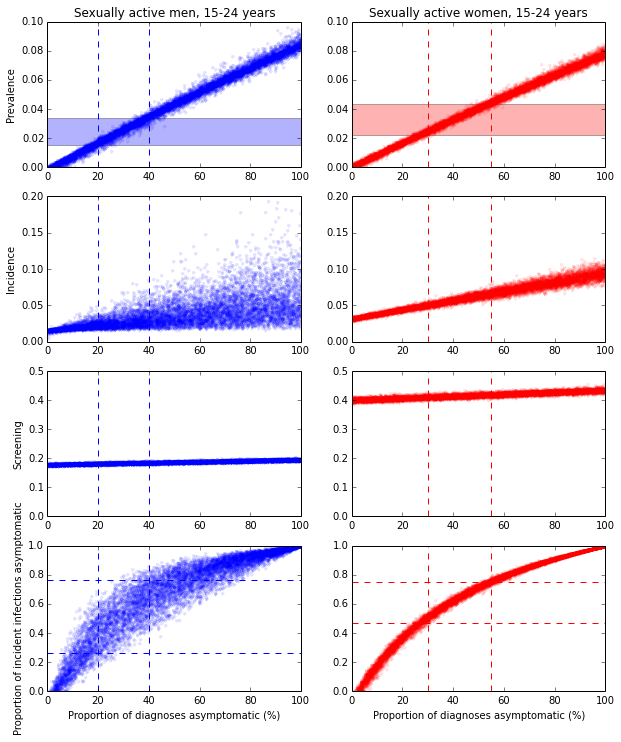
\includegraphics[width=15cm]{england_files/england_32_1.png}\end{center}
        \caption{Samples for prevalence, incidence, screening rate and proportion of infections which are symptomatic, assuming different proportions of diagnoses made as a result of symptomms. The dashed lines are intended as a guide to the eye, to indicate scenarios roughly compatible with the Natsal-3 prevalence estimates.}
        \label{fig:prev_samples_byage}
    \end{figure}
    
    The dashed lines are intended as a guide to the eye, to indicate
scenarios roughly compatible with the Natsal-3 prevalence estimates. The
observed chlamydia prevalence in Natsal-3 would be consistent with
around 60-80\% of diagnoses in men and 45-70\% in women being
symptomatic.

    \begin{footnotesize}
        \begin{Verbatim}[commandchars=\\\{\}]
{\color{incolor}In [{\color{incolor}24}]:} \PY{c}{\PYZsh{} Figure 6}
         \PY{c}{\PYZsh{} plot top pair only, for figure in paper}
         
         \PY{n}{fig} \PY{o}{=} \PY{n}{plt}\PY{o}{.}\PY{n}{figure}\PY{p}{(}\PY{n}{figsize} \PY{o}{=} \PY{p}{(}\PY{l+m+mi}{10}\PY{p}{,}\PY{l+m+mi}{3}\PY{p}{)}\PY{p}{)}
         
         \PY{n}{xtk\PYZus{}m} \PY{o}{=} \PY{p}{[}\PY{l+m+mi}{0}\PY{p}{,} \PY{l+m+mi}{10000}\PY{p}{,} \PY{l+m+mi}{20000}\PY{p}{,} \PY{l+m+mi}{30000}\PY{p}{,} \PY{l+m+mi}{40000}\PY{p}{]} \PY{c}{\PYZsh{} x\PYZhy{}axis ticks for men}
         \PY{n}{xtk\PYZus{}f} \PY{o}{=} \PY{p}{[}\PY{l+m+mi}{0}\PY{p}{,} \PY{l+m+mi}{20000}\PY{p}{,} \PY{l+m+mi}{40000}\PY{p}{,} \PY{l+m+mi}{60000}\PY{p}{,} \PY{l+m+mi}{80000}\PY{p}{]} \PY{c}{\PYZsh{} x\PYZhy{}axis ticks for women}
         
         \PY{n}{ax1} \PY{o}{=} \PY{n}{fig}\PY{o}{.}\PY{n}{add\PYZus{}subplot}\PY{p}{(}\PY{l+m+mi}{121}\PY{p}{)}
         \PY{n}{ax1}\PY{o}{.}\PY{n}{plot}\PY{p}{(}\PY{l+m+mi}{100}\PY{o}{*}\PY{p}{(}\PY{l+m+mi}{1}\PY{o}{\PYZhy{}}\PY{n}{sample\PYZus{}symp\PYZus{}m}\PY{o}{/}\PY{l+m+mi}{48387}\PY{p}{)}\PY{p}{,} \PY{n}{prev\PYZus{}m}\PY{p}{,} \PY{l+s}{\PYZsq{}}\PY{l+s}{.}\PY{l+s}{\PYZsq{}}\PY{p}{,} \PY{n}{alpha} \PY{o}{=} \PY{l+m+mf}{0.1}\PY{p}{)}
         \PY{n}{ax1}\PY{o}{.}\PY{n}{fill\PYZus{}between}\PY{p}{(}\PY{p}{[}\PY{l+m+mi}{0}\PY{p}{,}\PY{l+m+mi}{50000}\PY{p}{]}\PY{p}{,} \PY{l+m+mf}{0.015}\PY{p}{,} \PY{l+m+mf}{0.034}\PY{p}{,} \PY{n}{facecolor}\PY{o}{=}\PY{l+s}{\PYZsq{}}\PY{l+s}{b}\PY{l+s}{\PYZsq{}}\PY{p}{,} \PY{n}{alpha}\PY{o}{=}\PY{l+m+mf}{0.3}\PY{p}{)}
         \PY{n}{ax1}\PY{o}{.}\PY{n}{plot}\PY{p}{(}\PY{p}{[}\PY{l+m+mi}{40}\PY{p}{,}\PY{l+m+mi}{40}\PY{p}{]}\PY{p}{,}\PY{p}{[}\PY{l+m+mi}{0}\PY{p}{,}\PY{l+m+mi}{1}\PY{p}{]}\PY{p}{,}\PY{l+s}{\PYZsq{}}\PY{l+s}{\PYZhy{}\PYZhy{}b}\PY{l+s}{\PYZsq{}}\PY{p}{)}
         \PY{n}{ax1}\PY{o}{.}\PY{n}{plot}\PY{p}{(}\PY{p}{[}\PY{l+m+mi}{20}\PY{p}{,}\PY{l+m+mi}{20}\PY{p}{]}\PY{p}{,}\PY{p}{[}\PY{l+m+mi}{0}\PY{p}{,}\PY{l+m+mi}{1}\PY{p}{]}\PY{p}{,}\PY{l+s}{\PYZsq{}}\PY{l+s}{\PYZhy{}\PYZhy{}b}\PY{l+s}{\PYZsq{}}\PY{p}{)}
         \PY{n}{ax1}\PY{o}{.}\PY{n}{set\PYZus{}xlim}\PY{p}{(}\PY{p}{[}\PY{l+m+mi}{0}\PY{p}{,}\PY{l+m+mi}{100}\PY{p}{]}\PY{p}{)}
         \PY{n}{ax1}\PY{o}{.}\PY{n}{set\PYZus{}ylim}\PY{p}{(}\PY{p}{[}\PY{l+m+mi}{0}\PY{p}{,}\PY{l+m+mf}{0.1}\PY{p}{]}\PY{p}{)}
         \PY{n}{ax1}\PY{o}{.}\PY{n}{set\PYZus{}xlabel}\PY{p}{(}\PY{l+s}{\PYZsq{}}\PY{l+s}{Proportion of diagnoses asymptomatic (}\PY{l+s}{\PYZpc{}}\PY{l+s}{)}\PY{l+s}{\PYZsq{}}\PY{p}{)}
         \PY{n}{ax1}\PY{o}{.}\PY{n}{set\PYZus{}ylabel}\PY{p}{(}\PY{l+s}{\PYZsq{}}\PY{l+s}{Prevalence}\PY{l+s}{\PYZsq{}}\PY{p}{)}
         \PY{n}{ax1}\PY{o}{.}\PY{n}{set\PYZus{}title}\PY{p}{(}\PY{l+s}{\PYZsq{}}\PY{l+s}{Sexually active men, 15\PYZhy{}24 years}\PY{l+s}{\PYZsq{}}\PY{p}{)}
         
         \PY{n}{ax2} \PY{o}{=} \PY{n}{fig}\PY{o}{.}\PY{n}{add\PYZus{}subplot}\PY{p}{(}\PY{l+m+mi}{122}\PY{p}{)}
         \PY{n}{ax2}\PY{o}{.}\PY{n}{plot}\PY{p}{(}\PY{l+m+mi}{100}\PY{o}{*}\PY{p}{(}\PY{l+m+mi}{1}\PY{o}{\PYZhy{}}\PY{n}{sample\PYZus{}symp\PYZus{}f}\PY{o}{/}\PY{l+m+mi}{88101}\PY{p}{)}\PY{p}{,} \PY{n}{prev\PYZus{}f}\PY{p}{,} \PY{l+s}{\PYZsq{}}\PY{l+s}{.r}\PY{l+s}{\PYZsq{}}\PY{p}{,} \PY{n}{alpha} \PY{o}{=} \PY{l+m+mf}{0.1}\PY{p}{)}
         \PY{n}{ax2}\PY{o}{.}\PY{n}{fill\PYZus{}between}\PY{p}{(}\PY{p}{[}\PY{l+m+mi}{0}\PY{p}{,}\PY{l+m+mi}{100000}\PY{p}{]}\PY{p}{,} \PY{l+m+mf}{0.022}\PY{p}{,} \PY{l+m+mf}{0.043}\PY{p}{,} \PY{n}{facecolor}\PY{o}{=}\PY{l+s}{\PYZsq{}}\PY{l+s}{r}\PY{l+s}{\PYZsq{}}\PY{p}{,} \PY{n}{alpha}\PY{o}{=}\PY{l+m+mf}{0.3}\PY{p}{)}
         \PY{n}{ax2}\PY{o}{.}\PY{n}{plot}\PY{p}{(}\PY{p}{[}\PY{l+m+mi}{55}\PY{p}{,}\PY{l+m+mi}{55}\PY{p}{]}\PY{p}{,}\PY{p}{[}\PY{l+m+mi}{0}\PY{p}{,}\PY{l+m+mi}{1}\PY{p}{]}\PY{p}{,}\PY{l+s}{\PYZsq{}}\PY{l+s}{\PYZhy{}\PYZhy{}r}\PY{l+s}{\PYZsq{}}\PY{p}{)}
         \PY{n}{ax2}\PY{o}{.}\PY{n}{plot}\PY{p}{(}\PY{p}{[}\PY{l+m+mi}{30}\PY{p}{,}\PY{l+m+mi}{30}\PY{p}{]}\PY{p}{,}\PY{p}{[}\PY{l+m+mi}{0}\PY{p}{,}\PY{l+m+mi}{1}\PY{p}{]}\PY{p}{,}\PY{l+s}{\PYZsq{}}\PY{l+s}{\PYZhy{}\PYZhy{}r}\PY{l+s}{\PYZsq{}}\PY{p}{)}
         \PY{n}{ax2}\PY{o}{.}\PY{n}{set\PYZus{}xlim}\PY{p}{(}\PY{p}{[}\PY{l+m+mi}{0}\PY{p}{,}\PY{l+m+mi}{100}\PY{p}{]}\PY{p}{)}
         \PY{n}{ax2}\PY{o}{.}\PY{n}{set\PYZus{}ylim}\PY{p}{(}\PY{p}{[}\PY{l+m+mi}{0}\PY{p}{,}\PY{l+m+mf}{0.1}\PY{p}{]}\PY{p}{)}
         \PY{n}{ax2}\PY{o}{.}\PY{n}{set\PYZus{}xlabel}\PY{p}{(}\PY{l+s}{\PYZsq{}}\PY{l+s}{Proportion of diagnoses asymptomatic (}\PY{l+s}{\PYZpc{}}\PY{l+s}{)}\PY{l+s}{\PYZsq{}}\PY{p}{)}
         \PY{n}{ax2}\PY{o}{.}\PY{n}{set\PYZus{}title}\PY{p}{(}\PY{l+s}{\PYZsq{}}\PY{l+s}{Sexually active women, 15\PYZhy{}24 years}\PY{l+s}{\PYZsq{}}\PY{p}{)}
\end{Verbatim}
    \end{footnotesize}

    \begin{footnotesize}
            \begin{Verbatim}[commandchars=\\\{\}]
{\color{outcolor}Out[{\color{outcolor}24}]:} <matplotlib.text.Text at 0x111c175d0>
\end{Verbatim}
    \end{footnotesize}
        
    \begin{figure}
        \begin{center}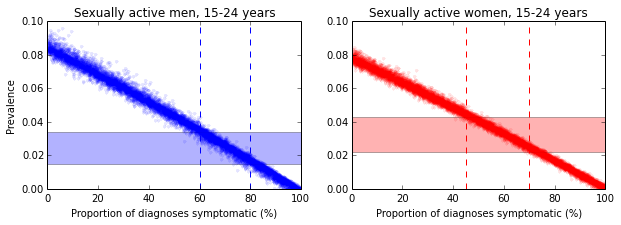
\includegraphics[width=15cm]{england_files/england_34_1.png}\end{center}
        \caption{The upper two panels from the previous figure.}
        \label{fig:prev_samples_byage}
    \end{figure}
    
    \begin{footnotesize}
        \begin{Verbatim}[commandchars=\\\{\}]
{\color{incolor}In [{\color{incolor} }]:} 
\end{Verbatim}
    \end{footnotesize}


    % Add a bibliography block to the postdoc
    
    
    
    \end{document}
